% Chapter Template

\chapter{1-D Memristor Simulation} % Main chapter title

\label{Chapter5} % Change X to a consecutive number; for referencing this chapter elsewhere, use \ref{ChapterX}

\lhead{Chapter 5. \emph{1-D Memristor Simulation}} % Change X to a consecutive number; this is for the header on each page - perhaps a shortened title

A numerical method for a memristor simulation was developed and tested in previous chapters based on drift-diffusion equations and finite difference. This chapter starts with the introduction of the memristor's structure and its physical parameters used for the simulation. It continues with a preliminary problem analysis to determine required mesh density and maximum possible time step. This preliminary analysis is followed by 1-D simulations of 3 different cross sections of a memristor.

\section{Memristor Structure}
%-Problem Analysis and assumptions, semiconductor vs memristor plots
Following figure (\ref{MemStc}) shows the structure of a simple memristor which will be taken as a basis for all the memristor simulations presented in this thesis. It consists of 2 metal contacts a polymer conductor (PEDOT:PSS) and an electrolyte solution which has lithium and perchlorate ions (6.02 $10^{26} m^{-3}$). The memristor is about 1 cm long. The thickness of the conductive layer is around 1 $\mu$m. During experimentation the electrolyte is deposited on PEDOT via a syringe so its thickness can vary drastically but as long as the amount of ions in the electrolyte solution is enough to saturate PEDOT this does not make a significant difference in the operation of the memristor. For simulation it was assumed that there were always more than enough ions to saturate the PEDOT so the electrolyte was modeled as an infinite source/sink of ions. The top boundary of the electrolyte was assumed to be charge neutral at all times which provides a mechanism for moving ions in and out of the system. This way the movement of ions near the surface of the PEDOT can still be captured without having to simulate the ion movement for the entire electrolyte solution which is variable in size. 

PEDOT:PSS is a regular conductor with fixed negative charge and mobile holes. Holes can move in an out of the PEDOT through the metal contacts. The interface between PEDOT and electrolyte only allows the exchange of lithium ions. The movement of lithium ions into the PEDOT changes the conductivity of the material by increasing or decreasing the amount of available holes through coulomb forces. In the actual device lithium ions change the conductivity via various physical effects like changing the mobility of holes through modifying their hopping distance. These additional affects are beyond the scope of this thesis. 

%-Details on Boundary conditions, boundary values, initial values, physical constants 
%-Wet/Dry pedot

\begin{figure}[!htp]
\centering
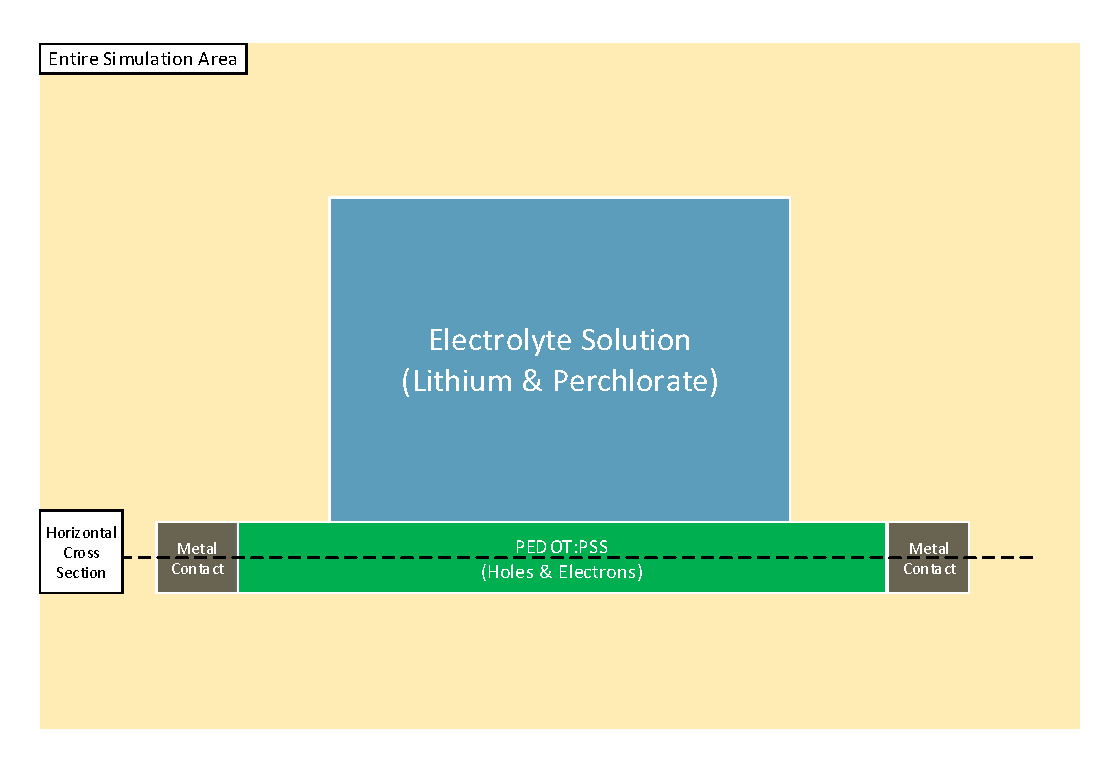
\includegraphics[scale=0.50]{Mem1}
\caption{} 
\label{MemStc}
\end{figure}

\clearpage
\section{Simulation Requirements}

It is important to analyze computational requirements of a simulation in order to asses the feasibility of the computation scheme. It is possible to determine these spacial and temporal requirements using the equations \ref{debye} to \ref{CFL_Drift} which describe physical and numerical limitations of the simulation. Following graph \ref{SpaceTime} shows the requirements for a memristor of the scale discussed above and a typical semiconductor device around 1 $\mu$m. The mesh density has to be high enough in order to capture the exponential charge accumulation for charge shielding so the minimum step size was set to be 5 times the Debye length. Plots \ref{SpaceTime}.a and \ref{SpaceTime}.c show the amount of points required to simulate a semiconductor and a memristor based on minimum step size. It is important to note that these values are for 1-D simulation and they can be converted to 2-D and 3-D by squaring or cubing y axis values respectively. Plots \ref{SpaceTime}.b and \ref{SpaceTime}.d were created using CFL conditions for drift and diffusion and dielectric relaxation time. A typical simulation time was estimated using mobility and electric field. Based on the estimated simulation time the number of time steps were calculated using the minimum time step obtained from CFL conditions and dielectric relaxation time.

It can be seen from graphs \ref{SpaceTime}.a and \ref{SpaceTime}.c that memristor simulations require much higher mesh densities compared to a typical semiconductor simulation. This is due to the larger size and higher charge density of the memristor. Graph \ref{SpaceTime}.a \ref{SpaceTime}.b show that a memristor with $10^{26}$ $m^{3}$ charge density of the electrolyte would require close to $10^9$ points and $10^{14}$ time steps to simulate in 1-D. These requirements make the simulation of the memristor extremely challenging. One possible solution to this problem is to use a much lower charge density and assume that all the values scale linearly. Following cross sectional simulations (Figure \ref{MemStc}) were made to determine the effect of increasing charge density on memristor simulations and to investigate if scaling can be used without compromising the reliability of the simulation.

\begin{landscape}
\begin{figure}[htp]
\centering
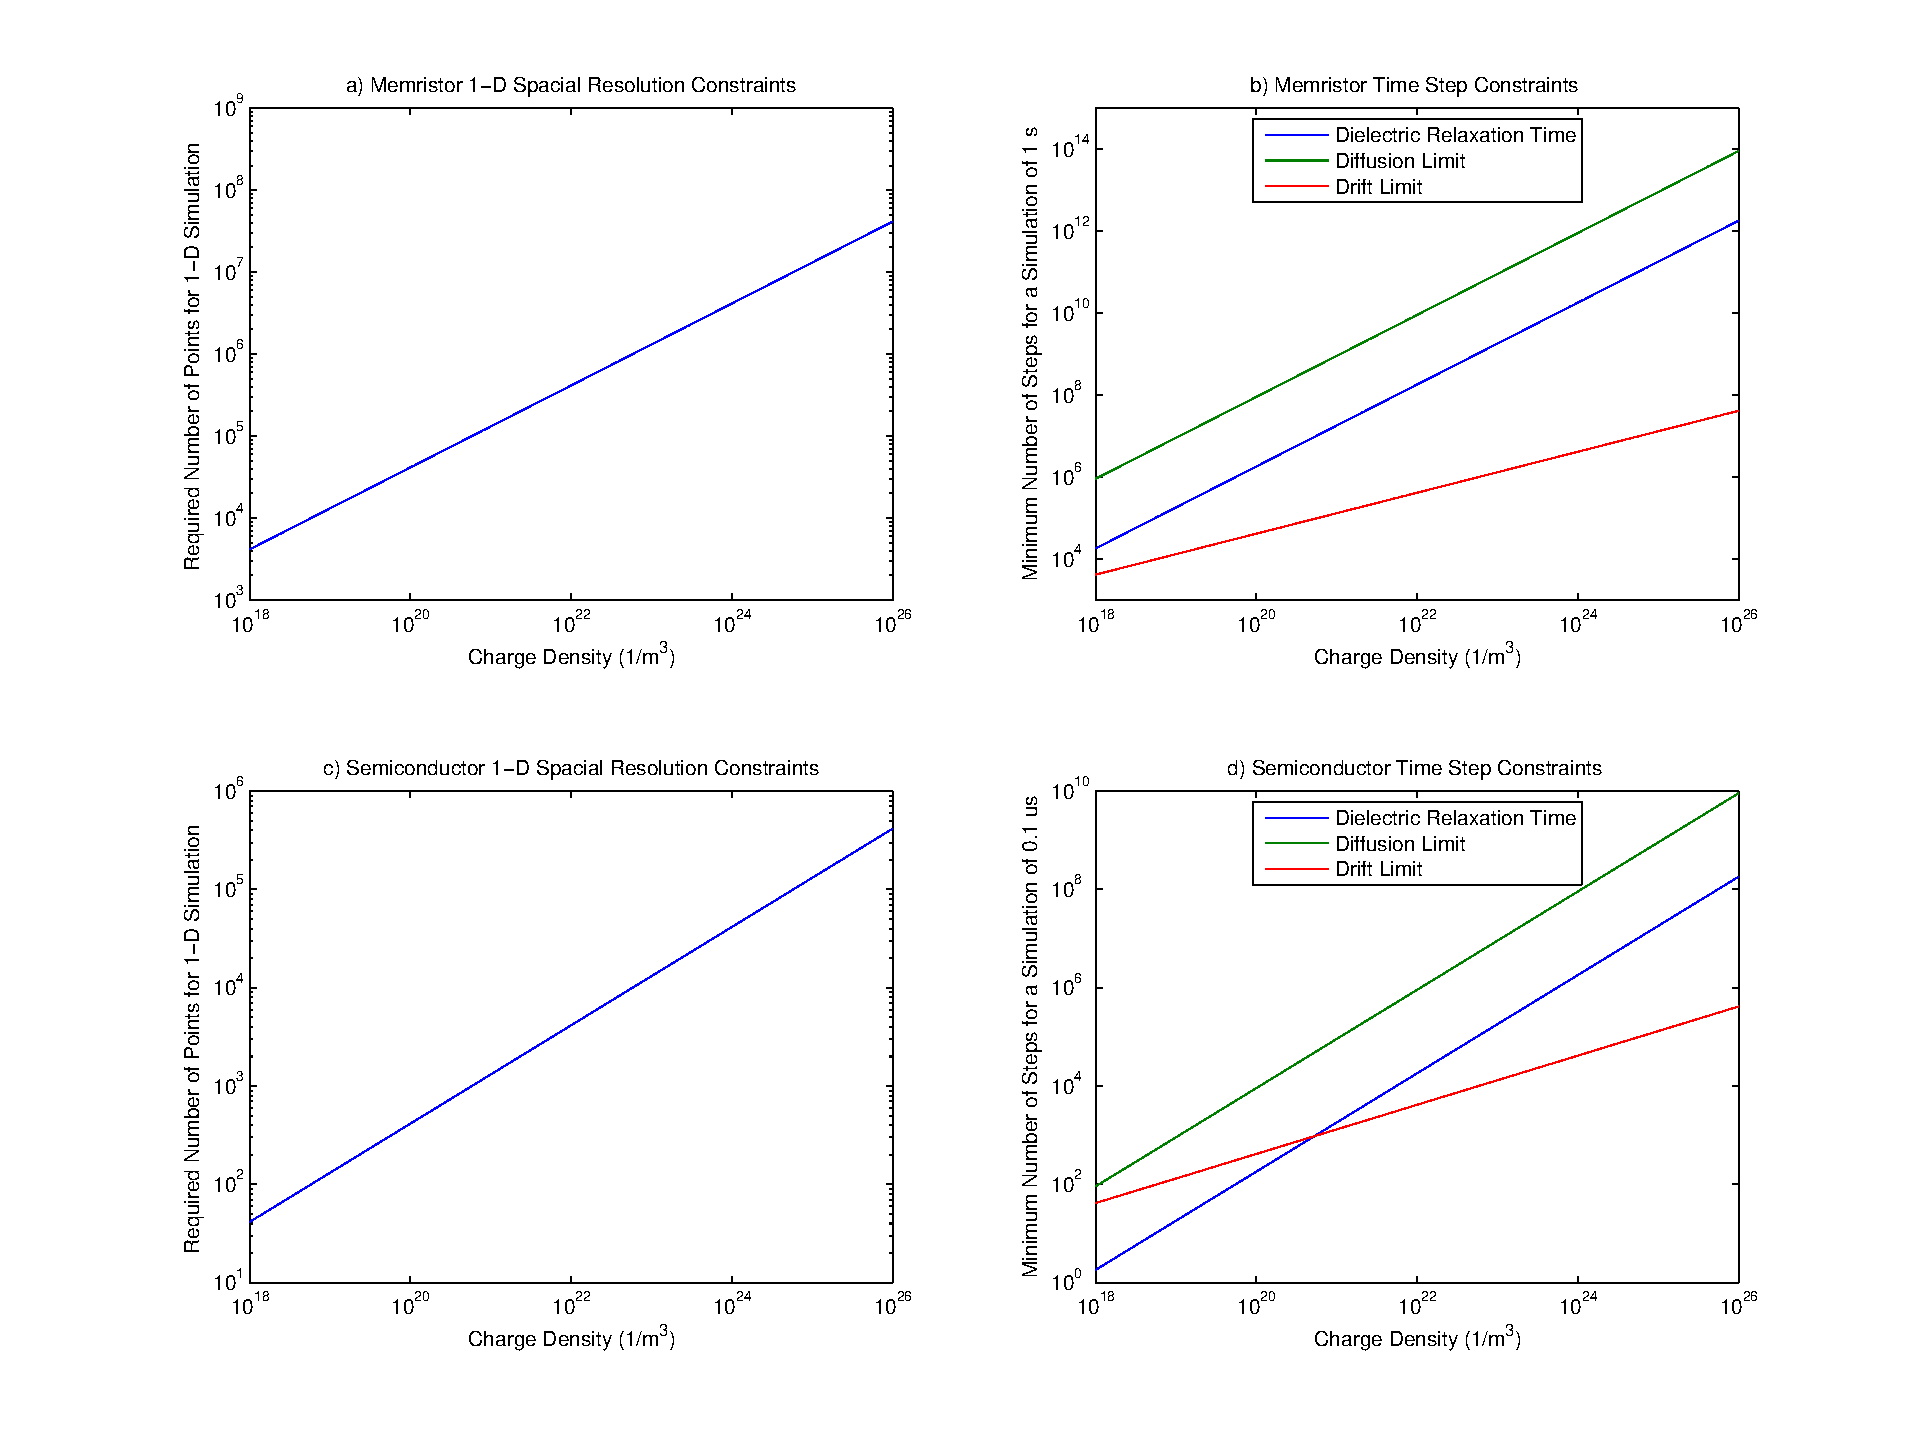
\includegraphics[scale=0.60]{SpaceTime}
\caption{} 
\label{SpaceTime}
\end{figure}
\end{landscape}

\clearpage
\section{Memristor Cross Sectional Simulations}

Even though it is possible to simulate the structure presented in section 5.1 in 2-D, simulating cross sections of the memristor separately has a major advantage. The purpose of these preliminary  simulations is to test the affect of various charge densities which requires mesh density to be as high as possible. Increasing mesh density in 1-D has a smaller impact on the total simulation time therefore higher charge densities are more accessible.  

\subsection{Electrolyte Simulation (Cross Section 1)}


\begin{figure}[!htp]
\centering
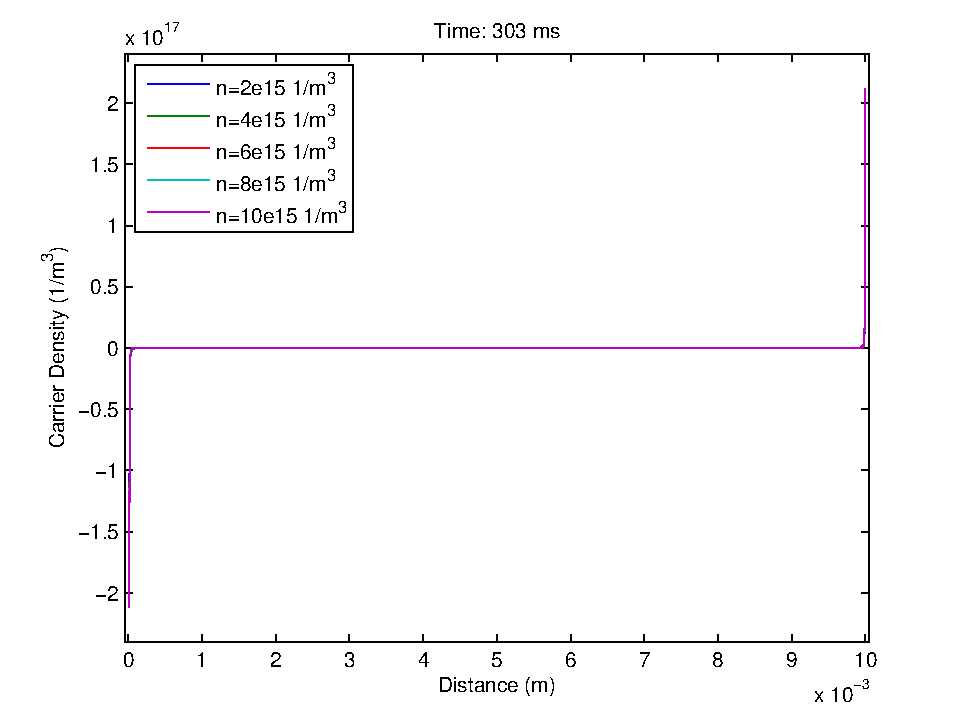
\includegraphics[scale=0.60]{Ex1NetQ_Time_All}
\caption{} 
\label{}
\end{figure}



\begin{landscape}
\begin{figure}[!htp]
\centering
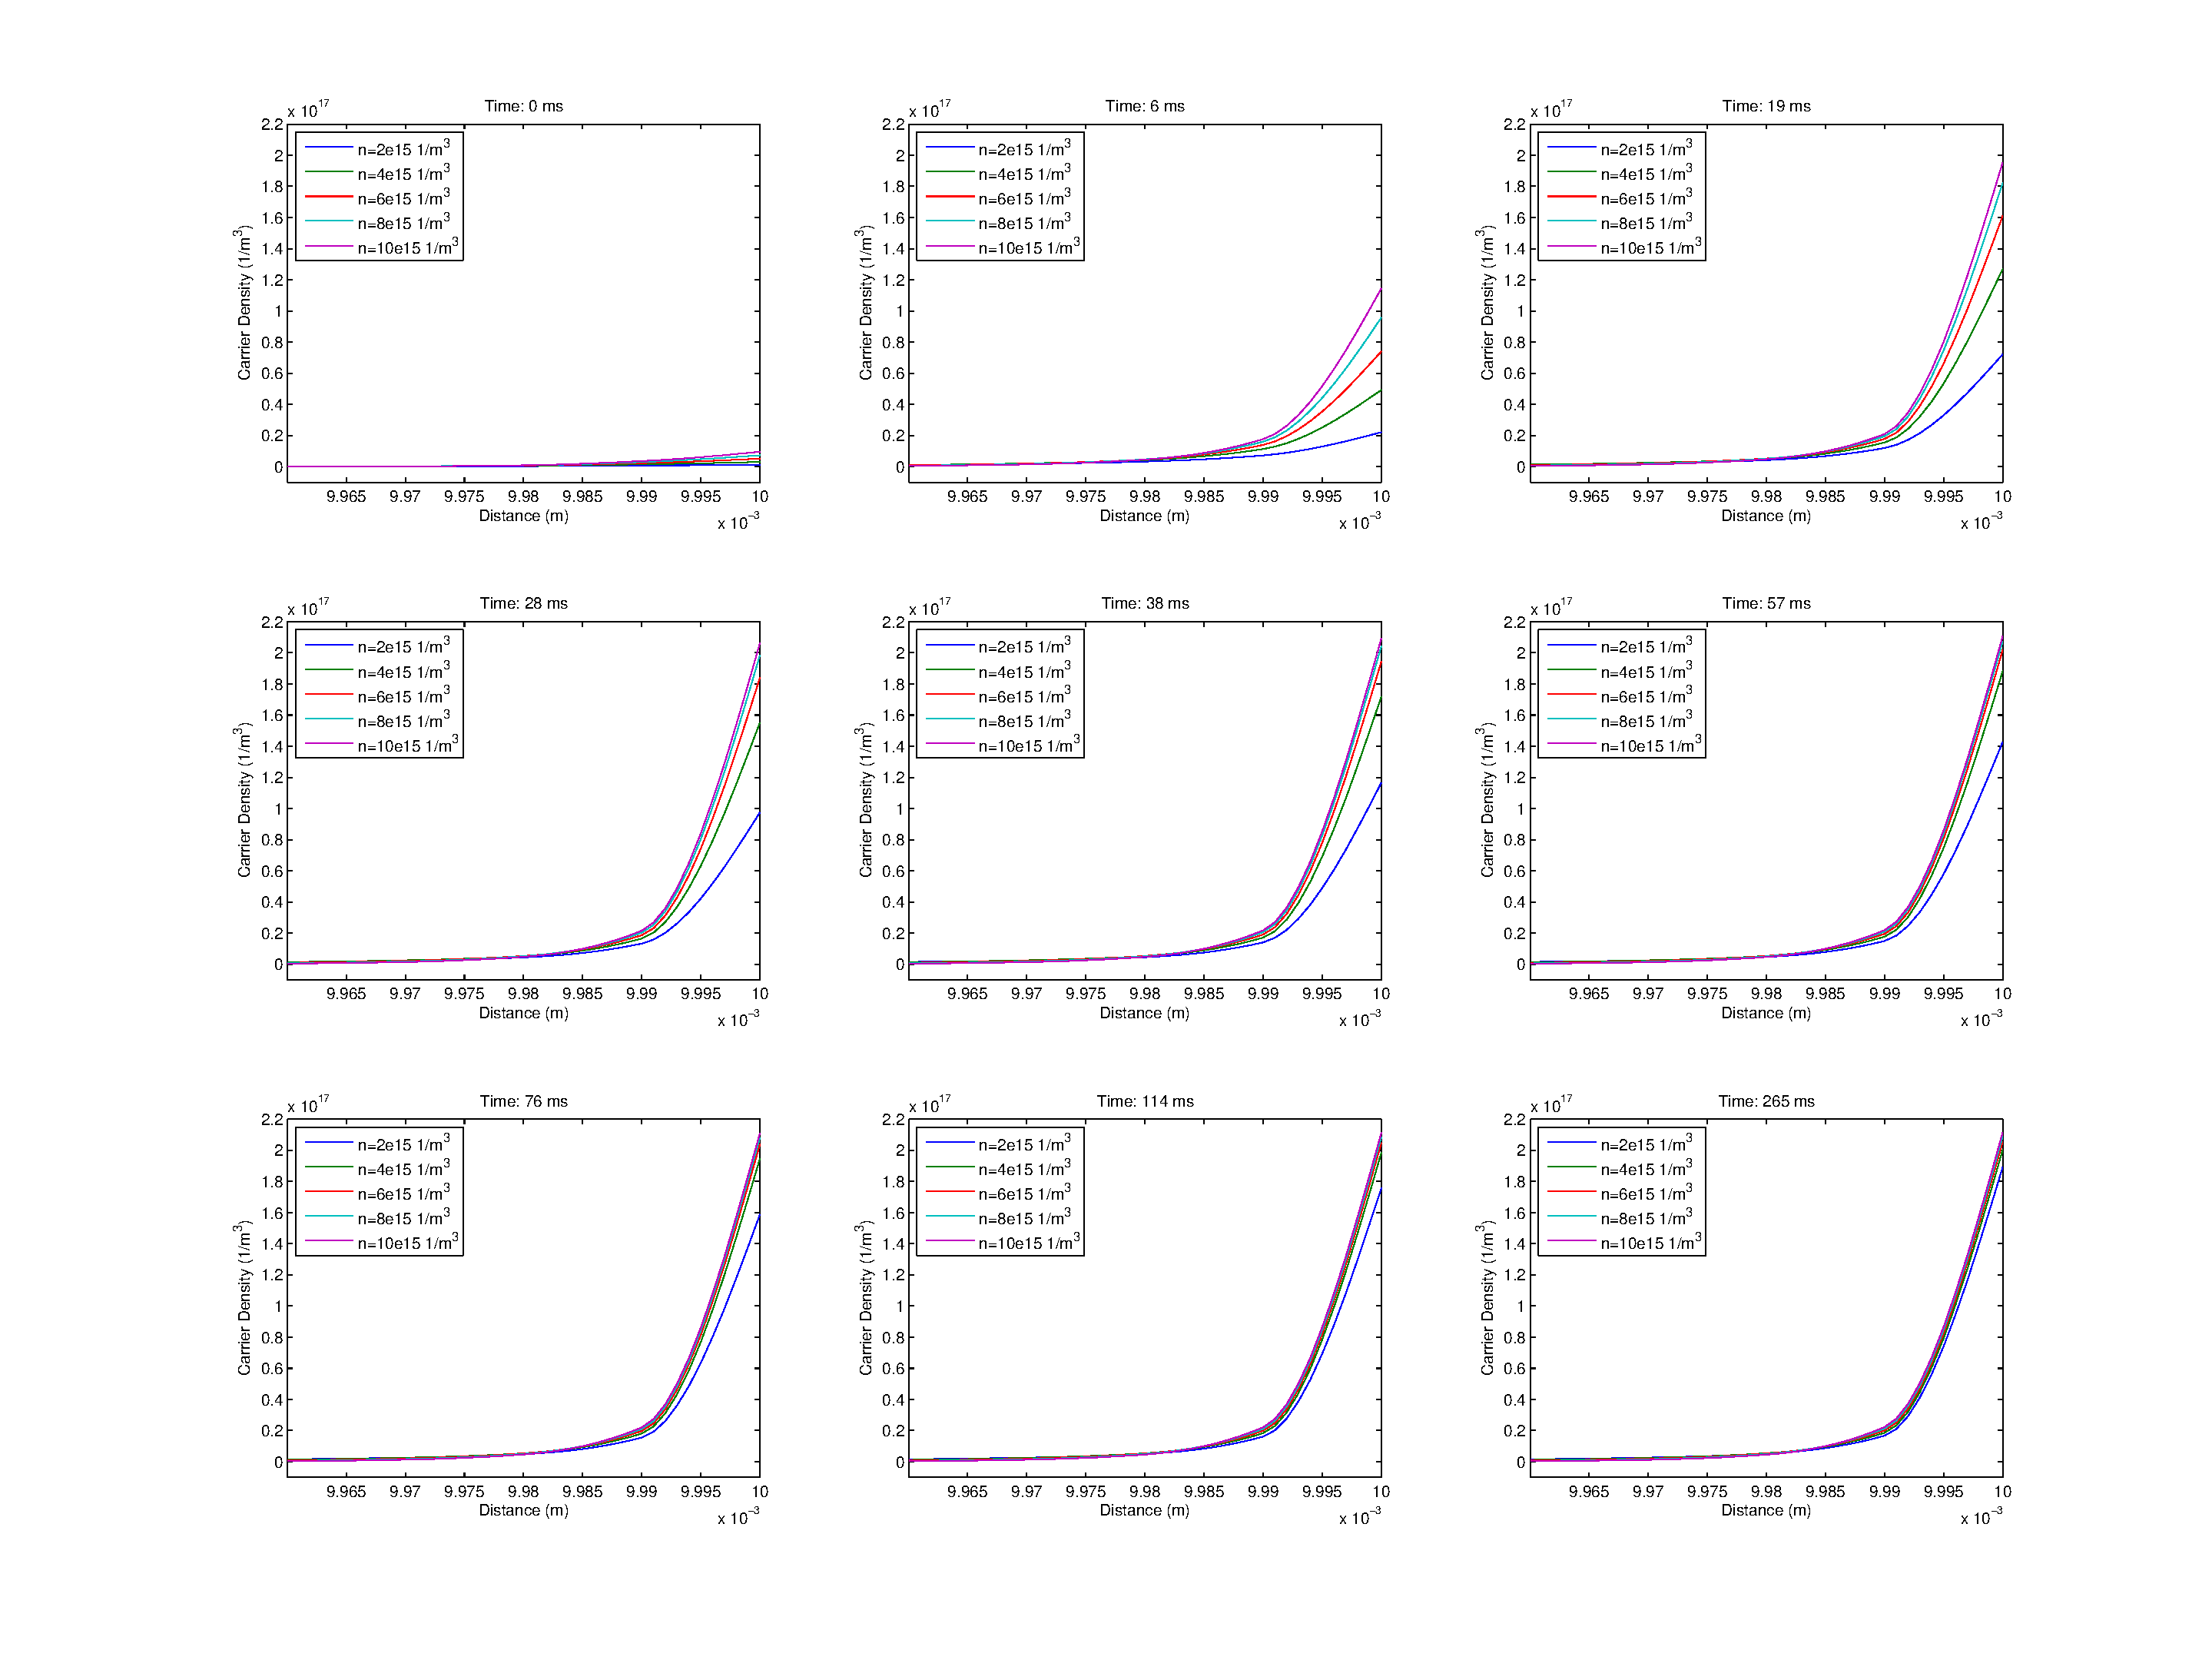
\includegraphics[scale=0.40]{Ex1NetQ_Time}
\caption{} 
\label{}
\end{figure}
\end{landscape}

\begin{landscape}
\begin{figure}[!htp]
\centering
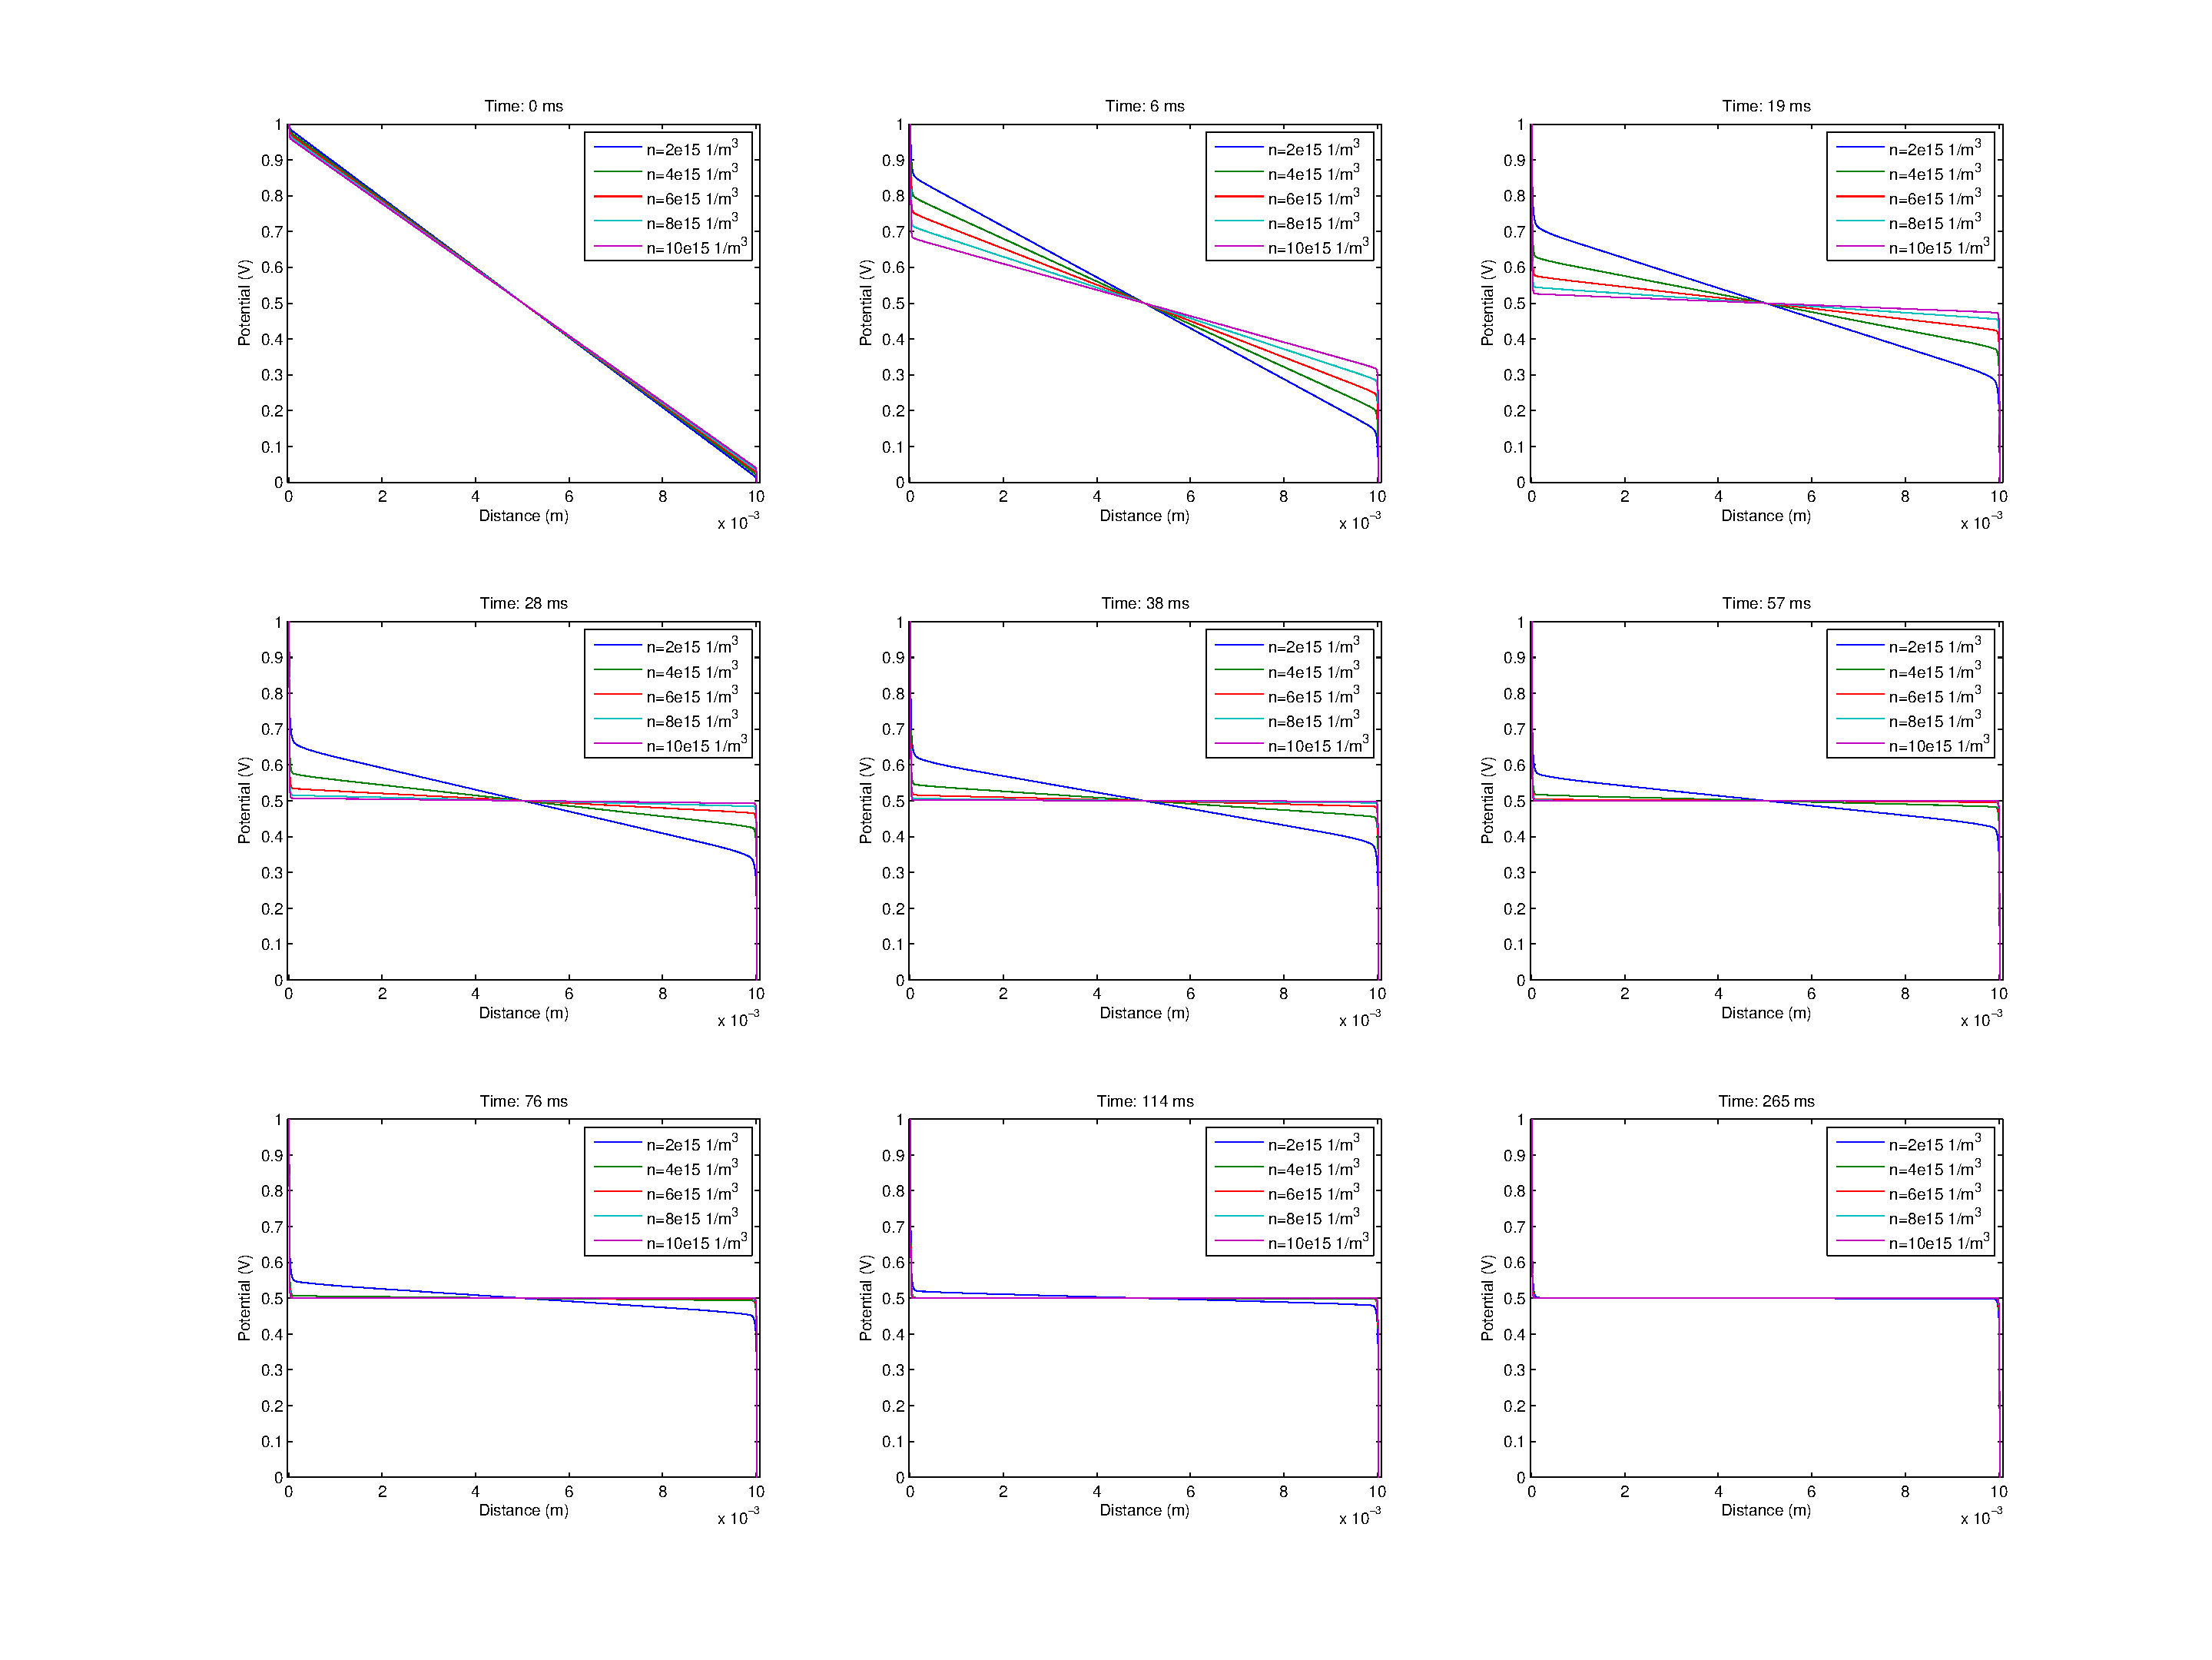
\includegraphics[scale=0.40]{Ex1V_Time}
\caption{} 
\label{}
\end{figure}
\end{landscape}

\begin{landscape}
\begin{figure}[!htp]
\centering
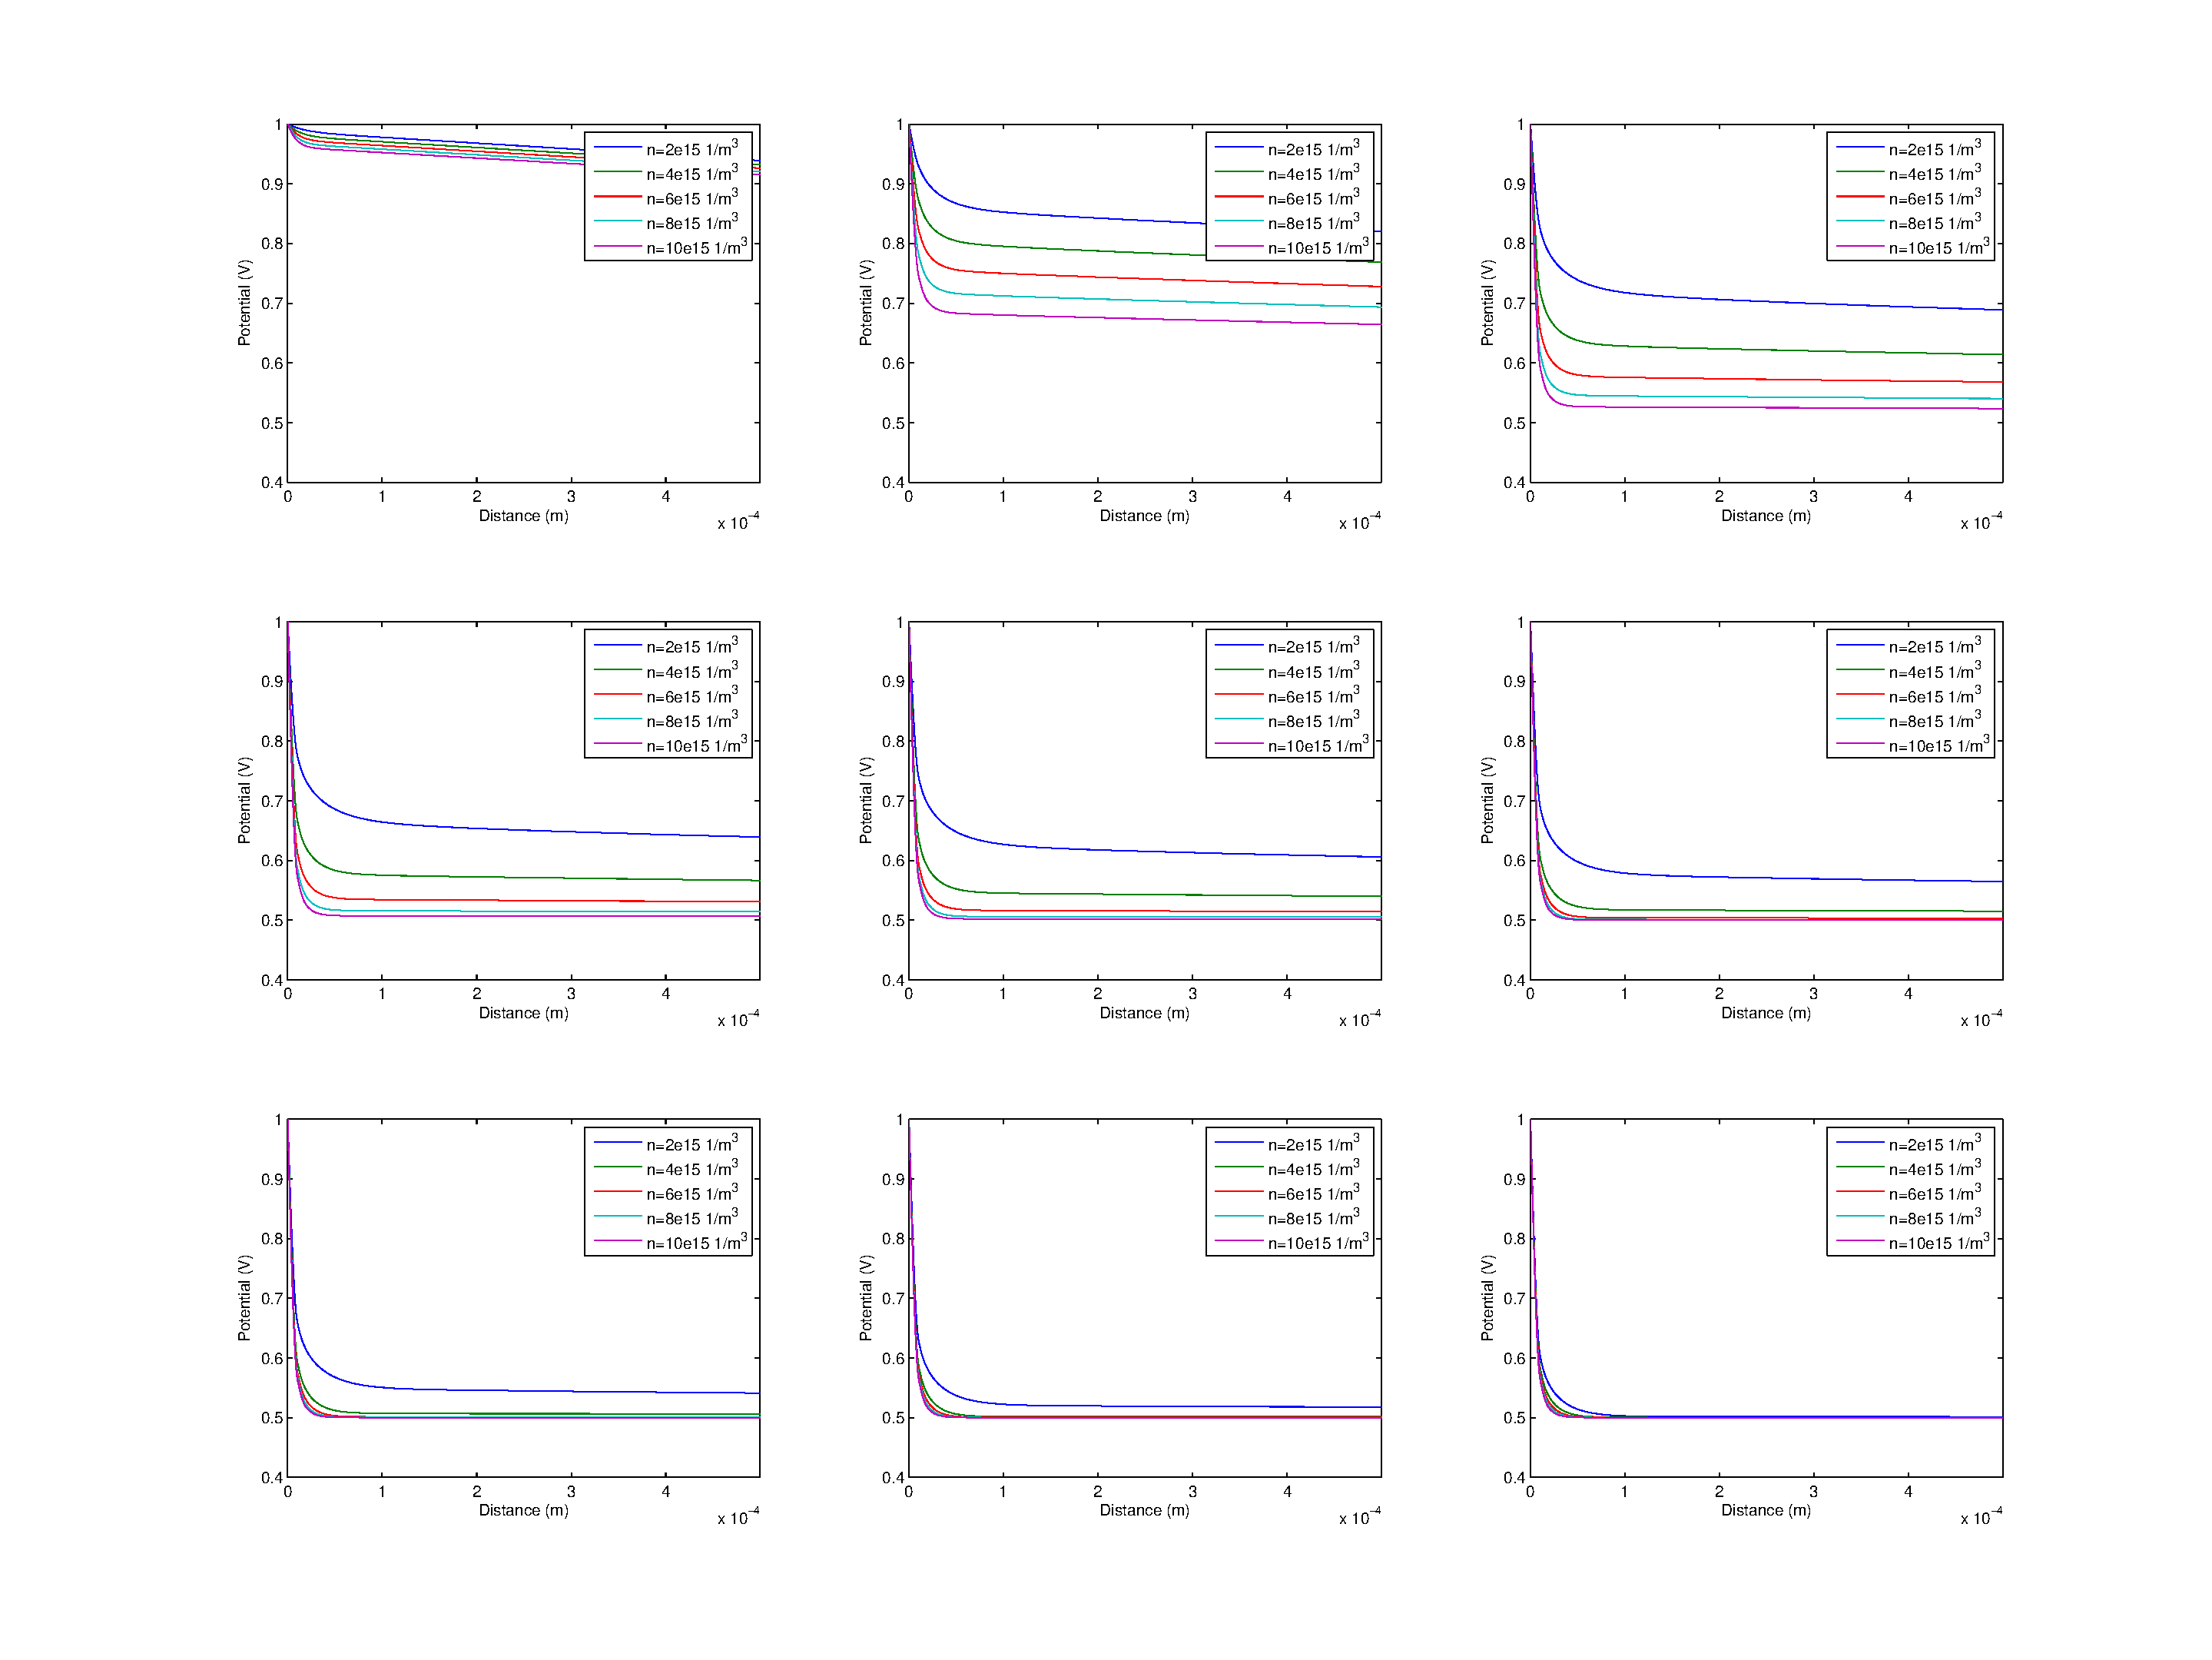
\includegraphics[scale=0.40]{Ex1V_Time2}
\caption{} 
\label{}
\end{figure}
\end{landscape}

\clearpage
\subsection{1-D Horizontal Memristor (Cross Section 2)}

\begin{figure}[!htp]
\centering
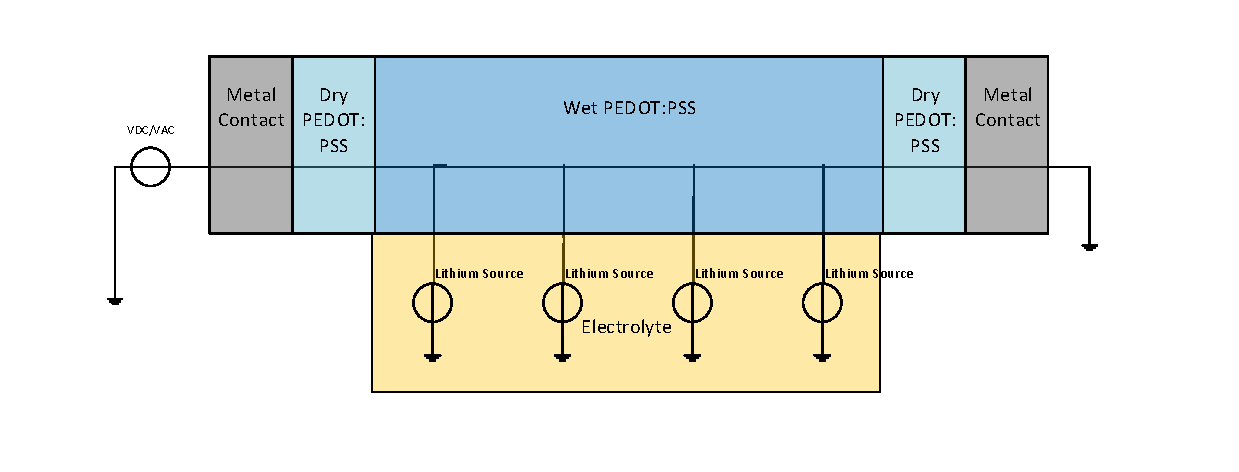
\includegraphics[scale=0.74]{1DMem}
\caption{} 
\label{}
\end{figure}


\begin{landscape}
\begin{figure}[!htp]
\centering
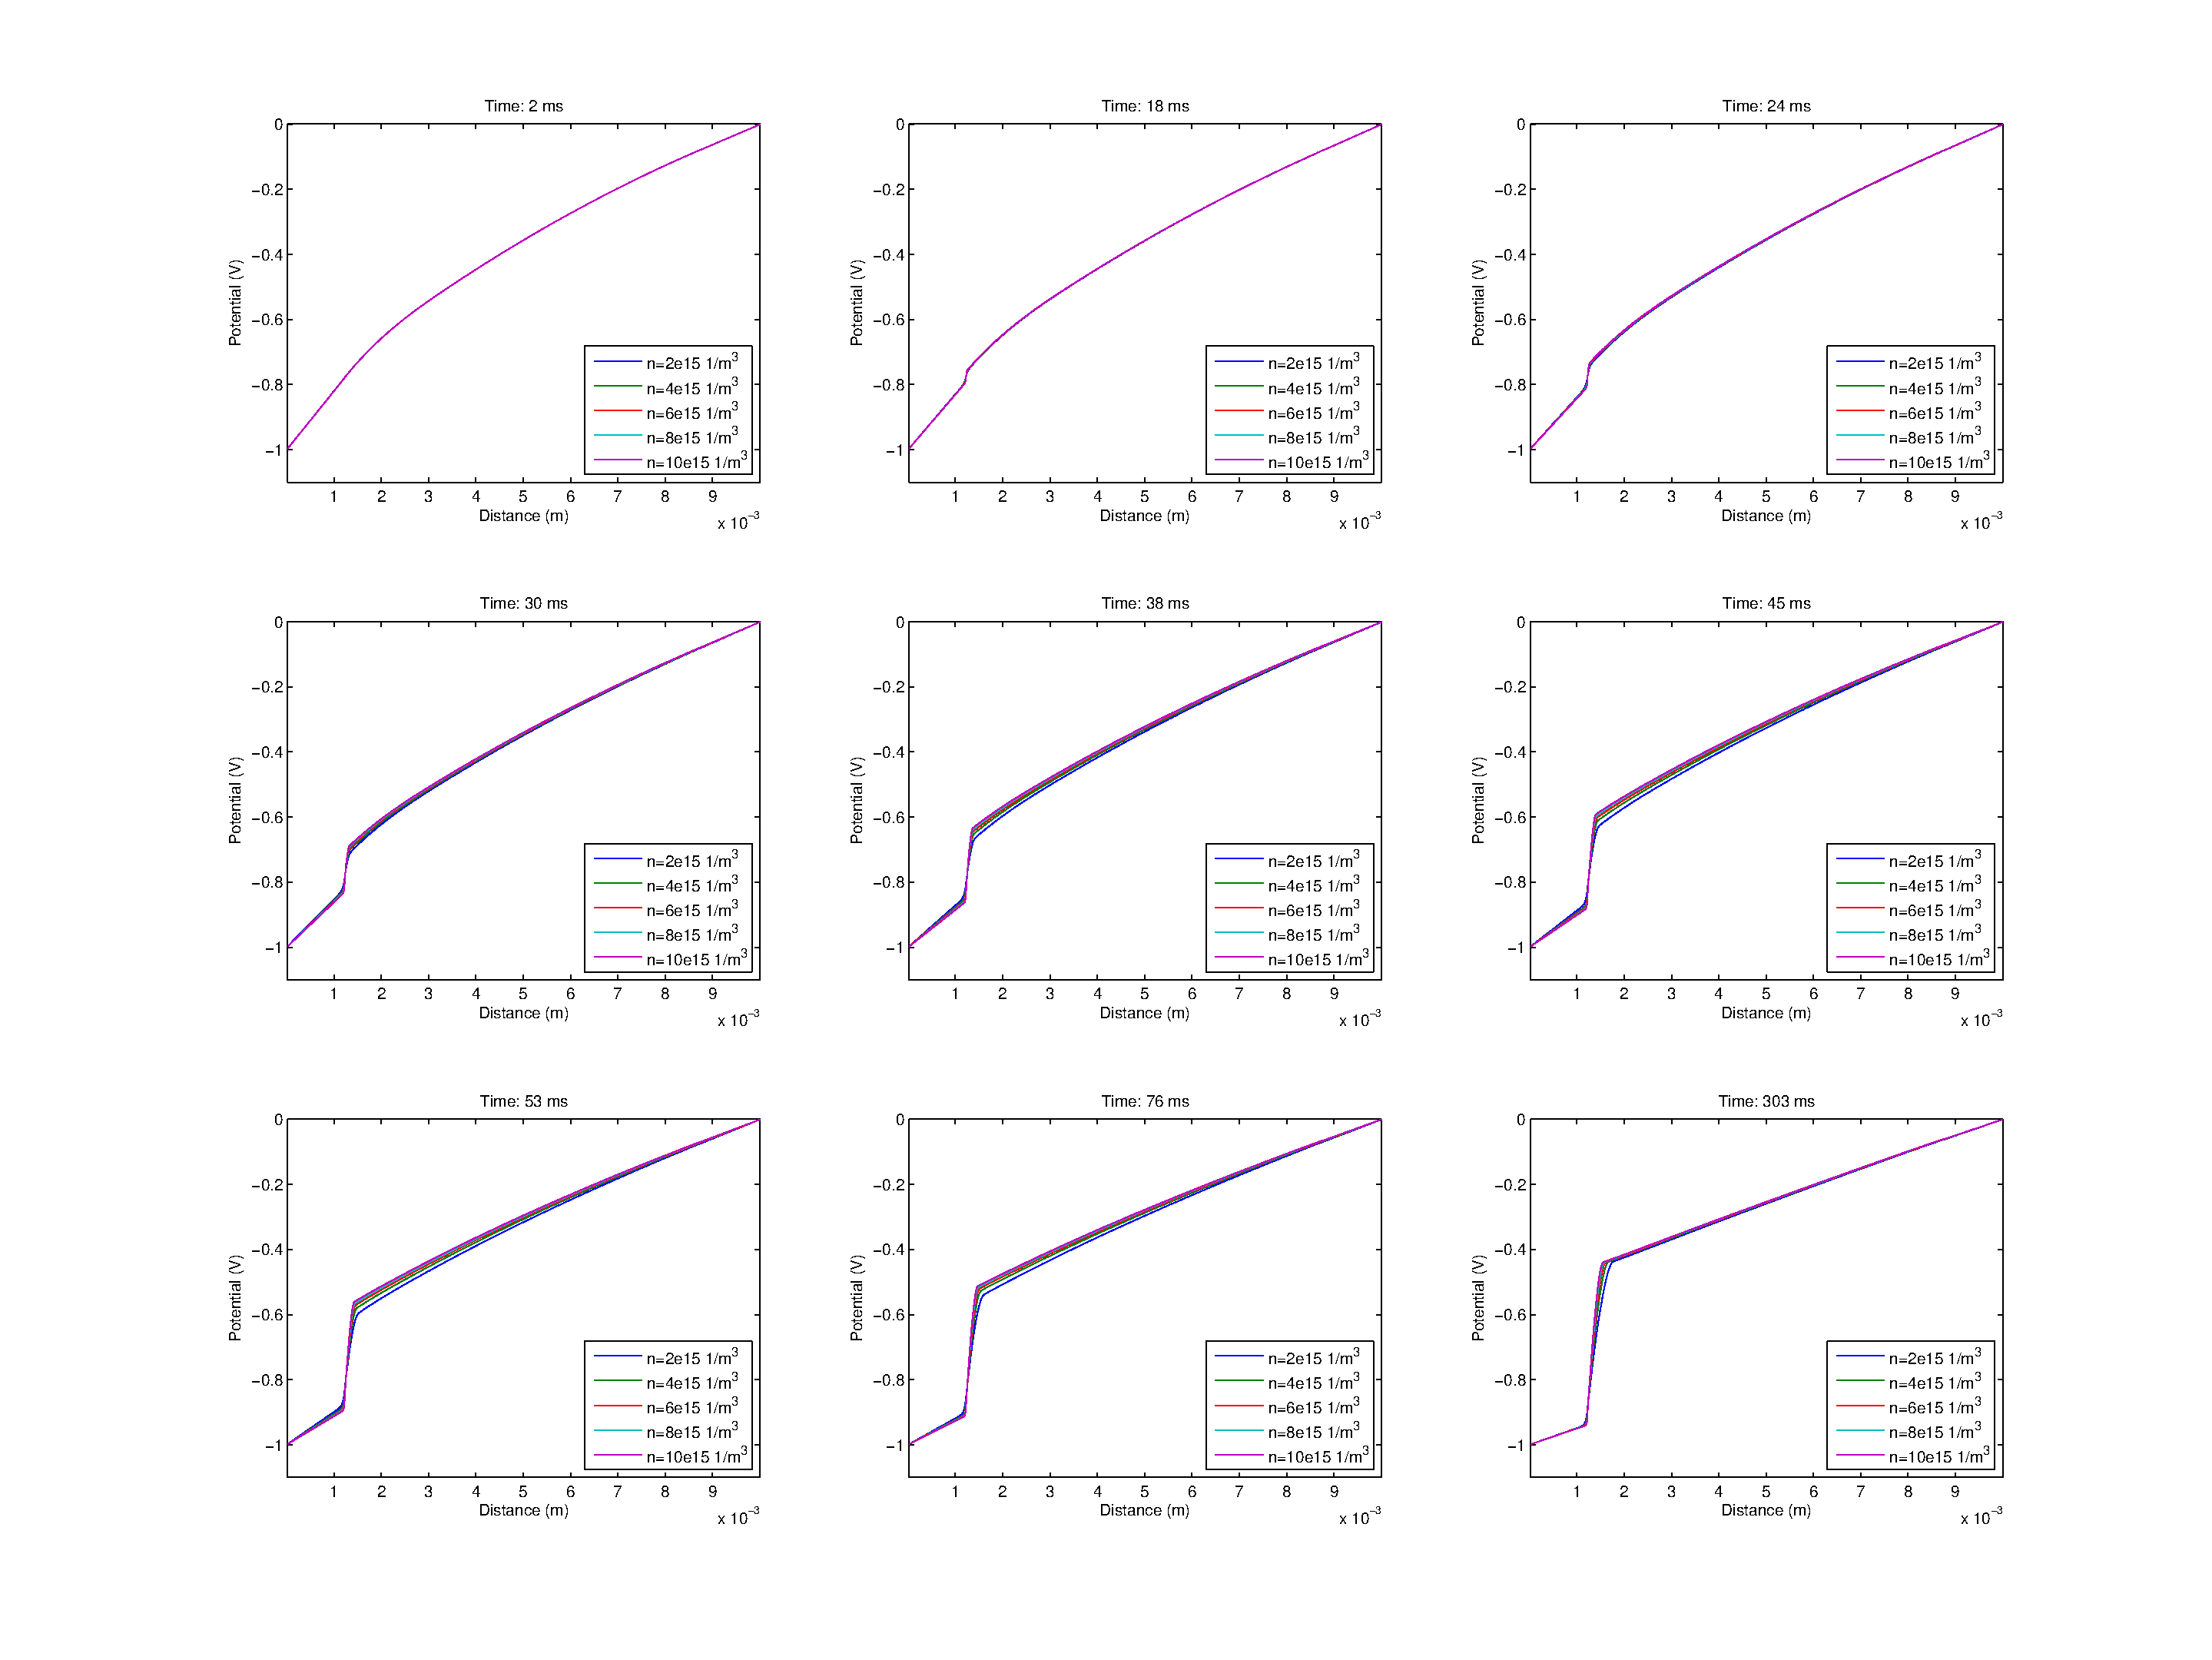
\includegraphics[scale=0.40]{Ex5V_Time1}
\caption{} 
\label{}
\end{figure}
\end{landscape}

\begin{landscape}
\begin{figure}[!htp]
\centering
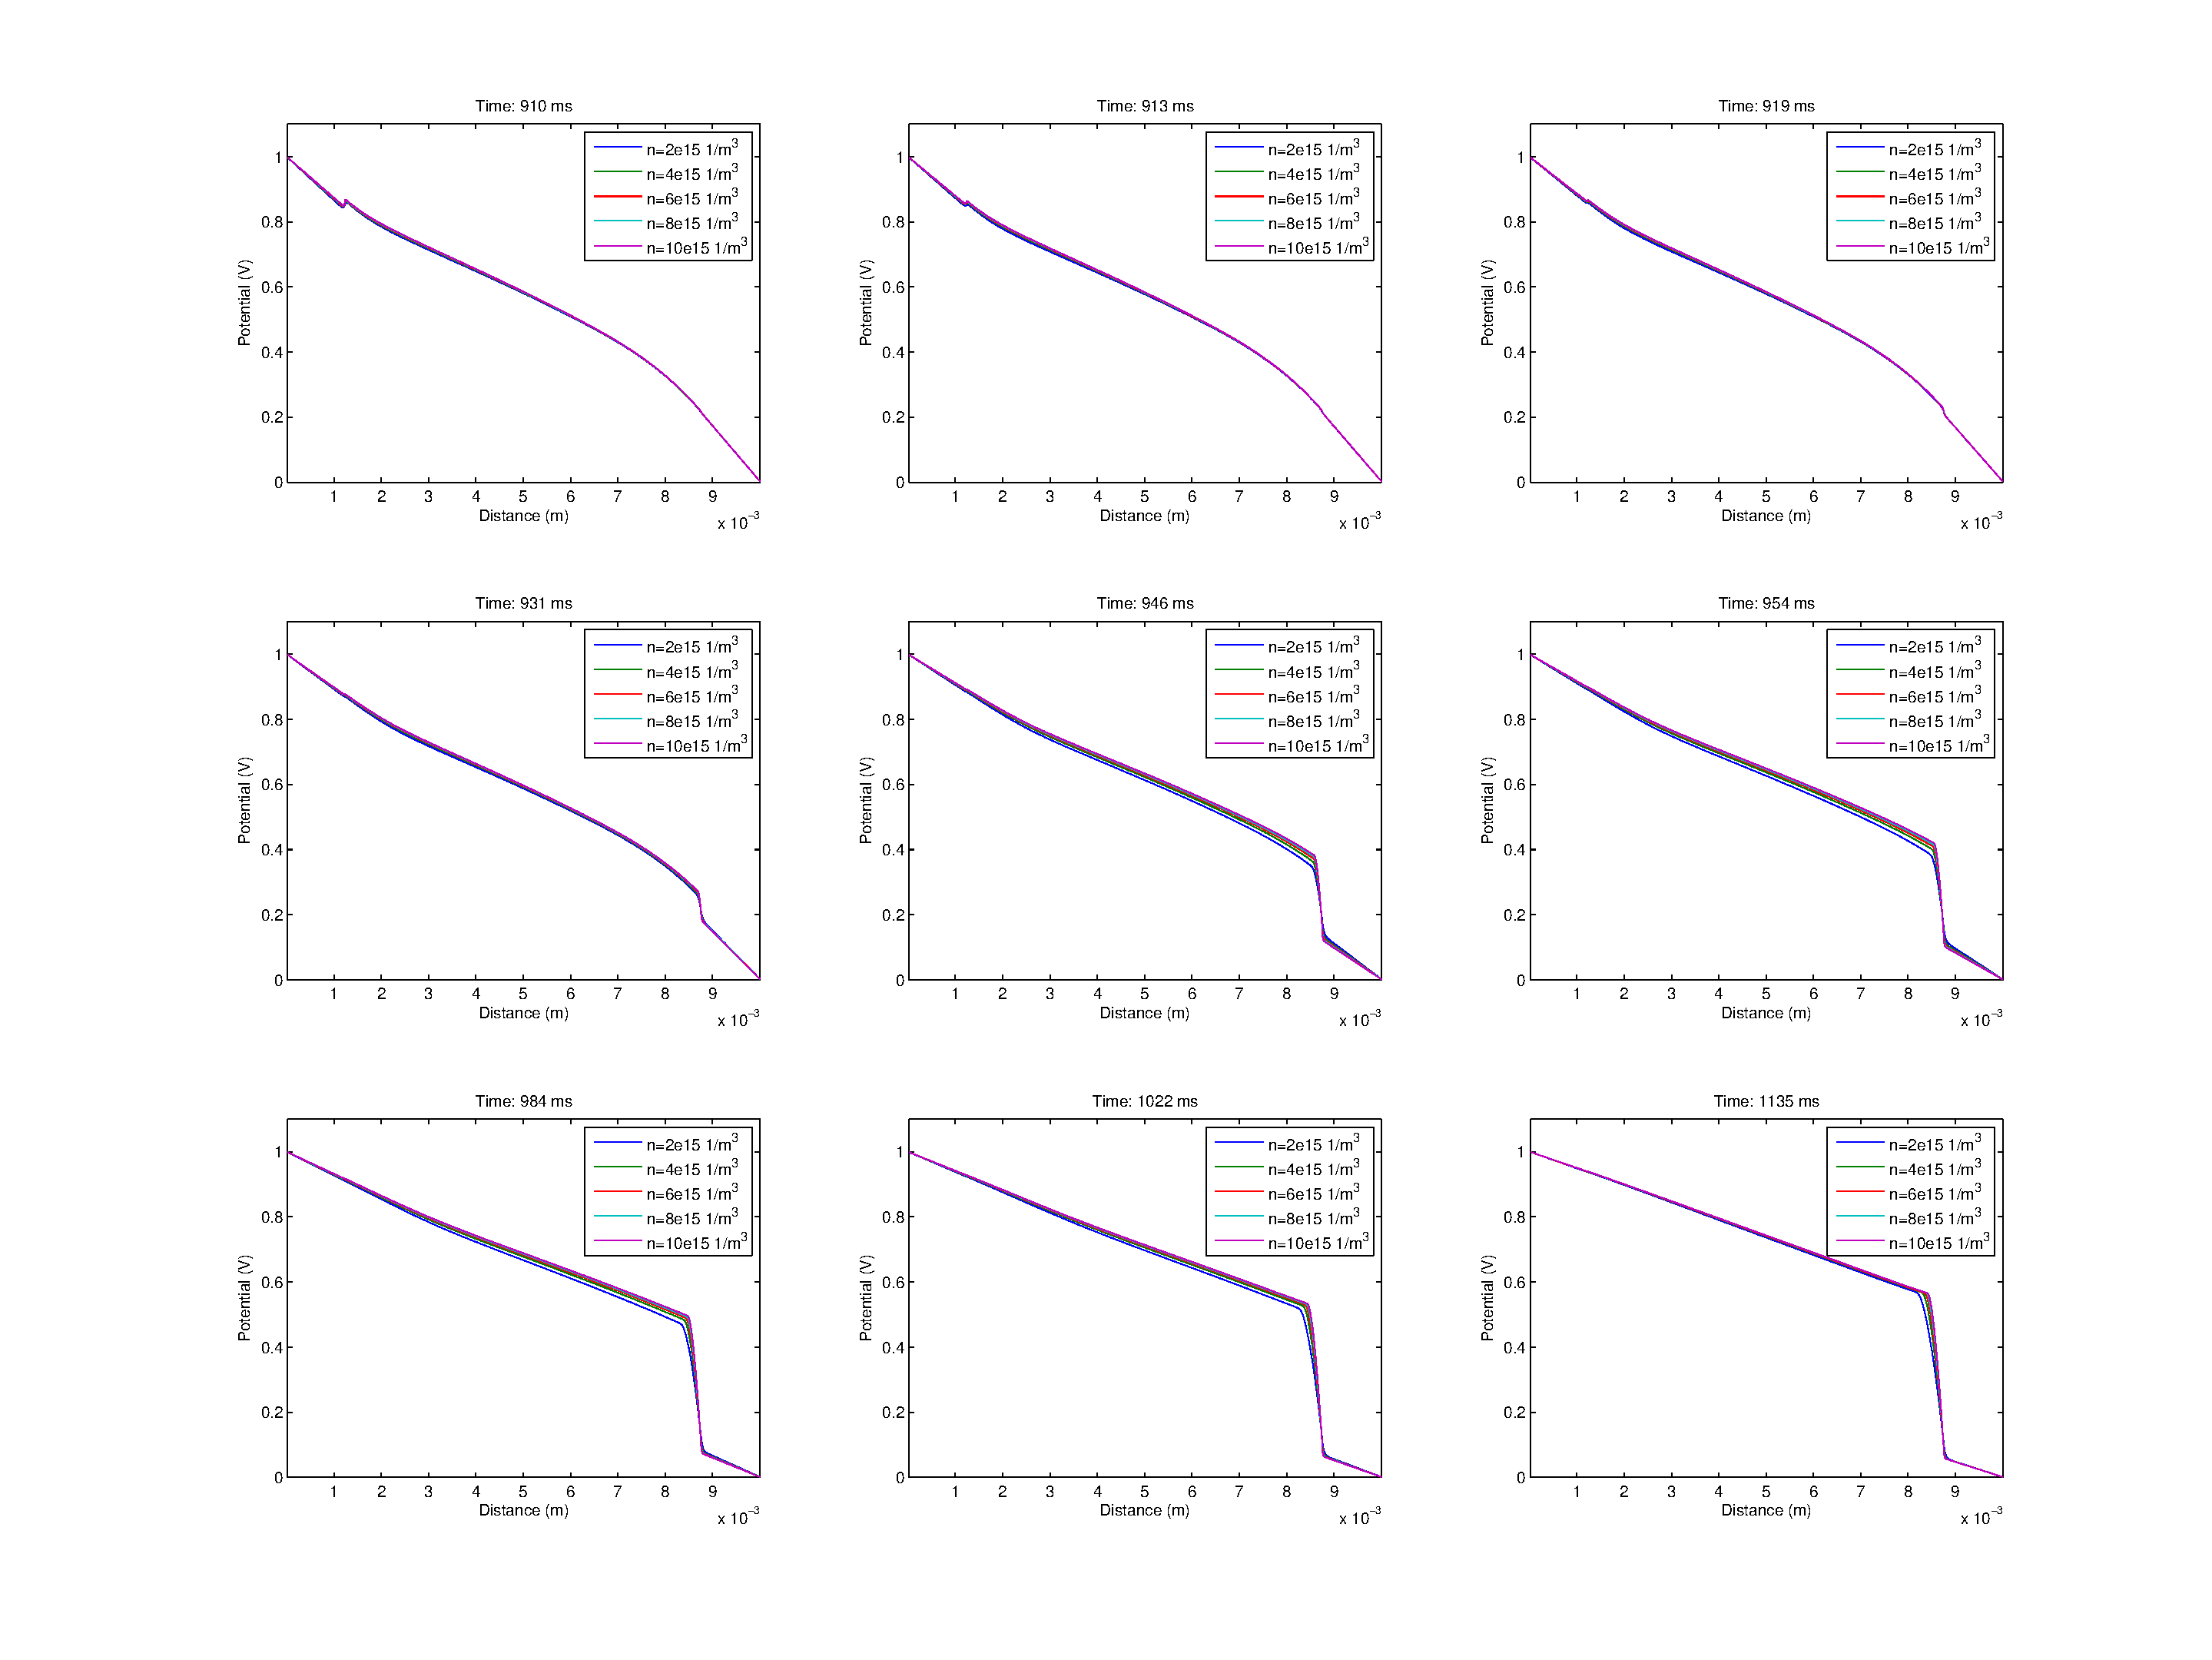
\includegraphics[scale=0.40]{Ex5V_Time2}
\caption{} 
\label{}
\end{figure}
\end{landscape}

\begin{landscape}
\begin{figure}[!htp]
\centering
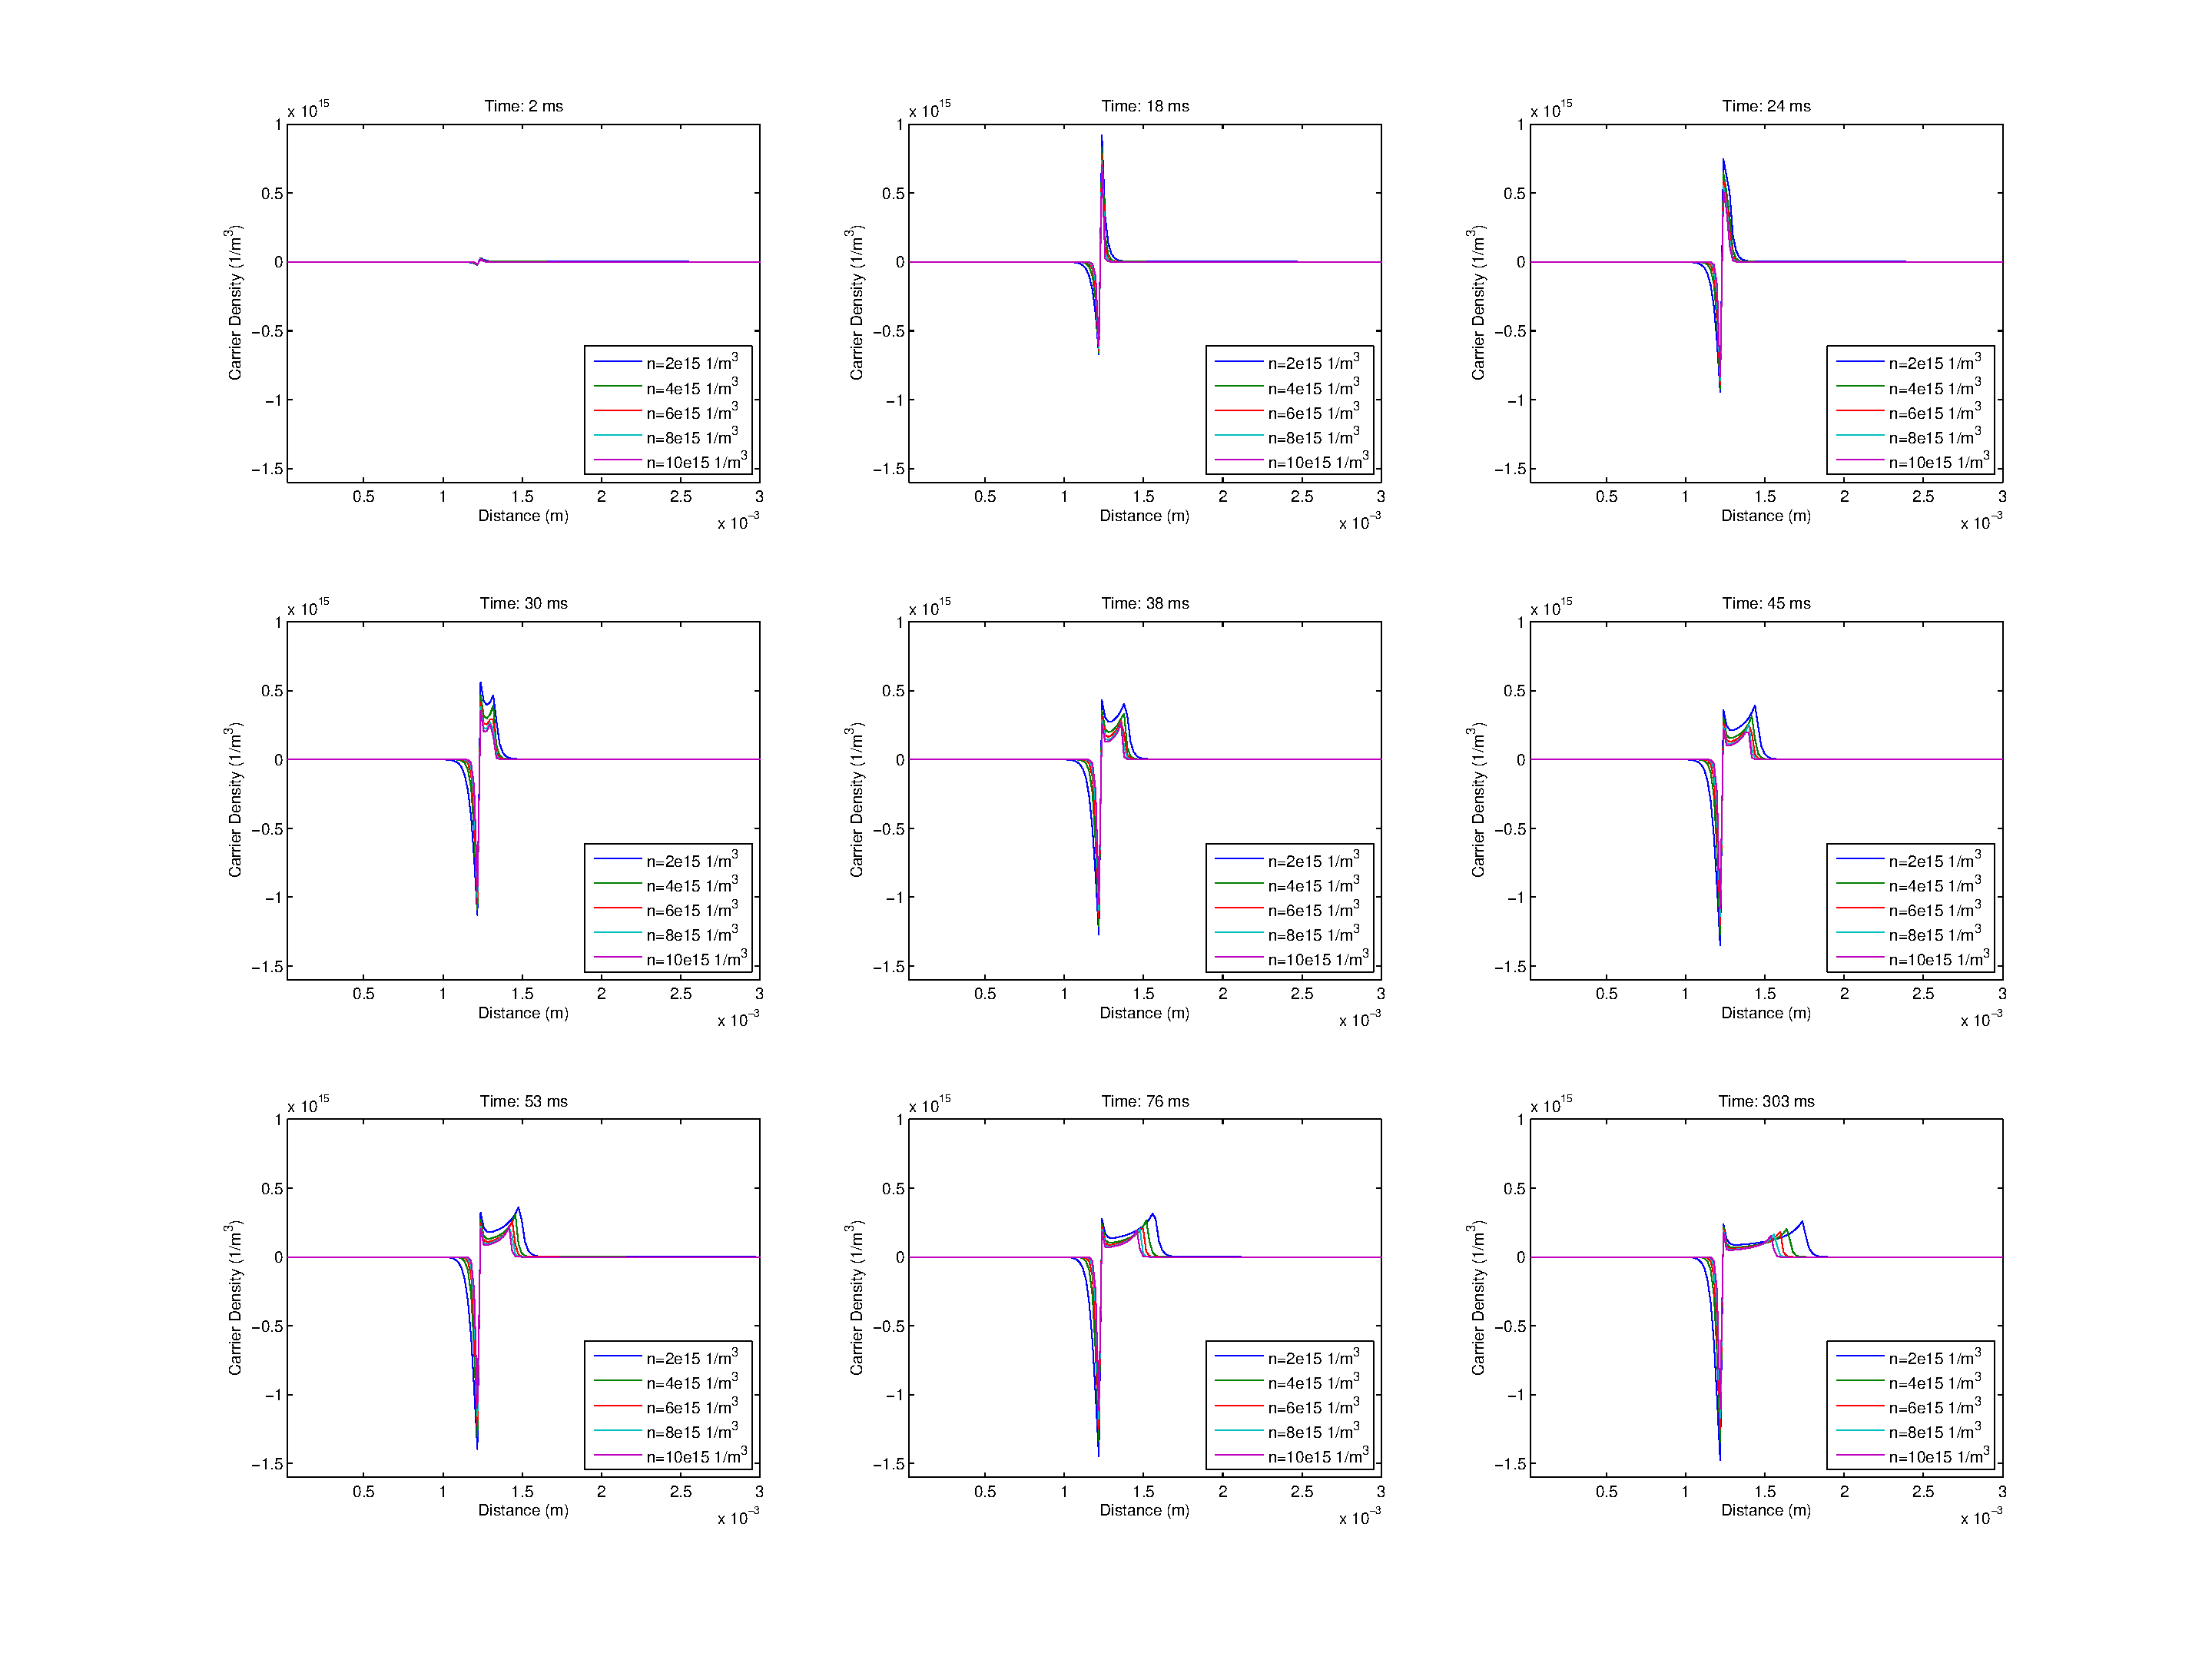
\includegraphics[scale=0.40]{Ex5NetQ_Time1}
\caption{} 
\label{}
\end{figure}
\end{landscape}

\begin{landscape}
\begin{figure}[!htp]
\centering
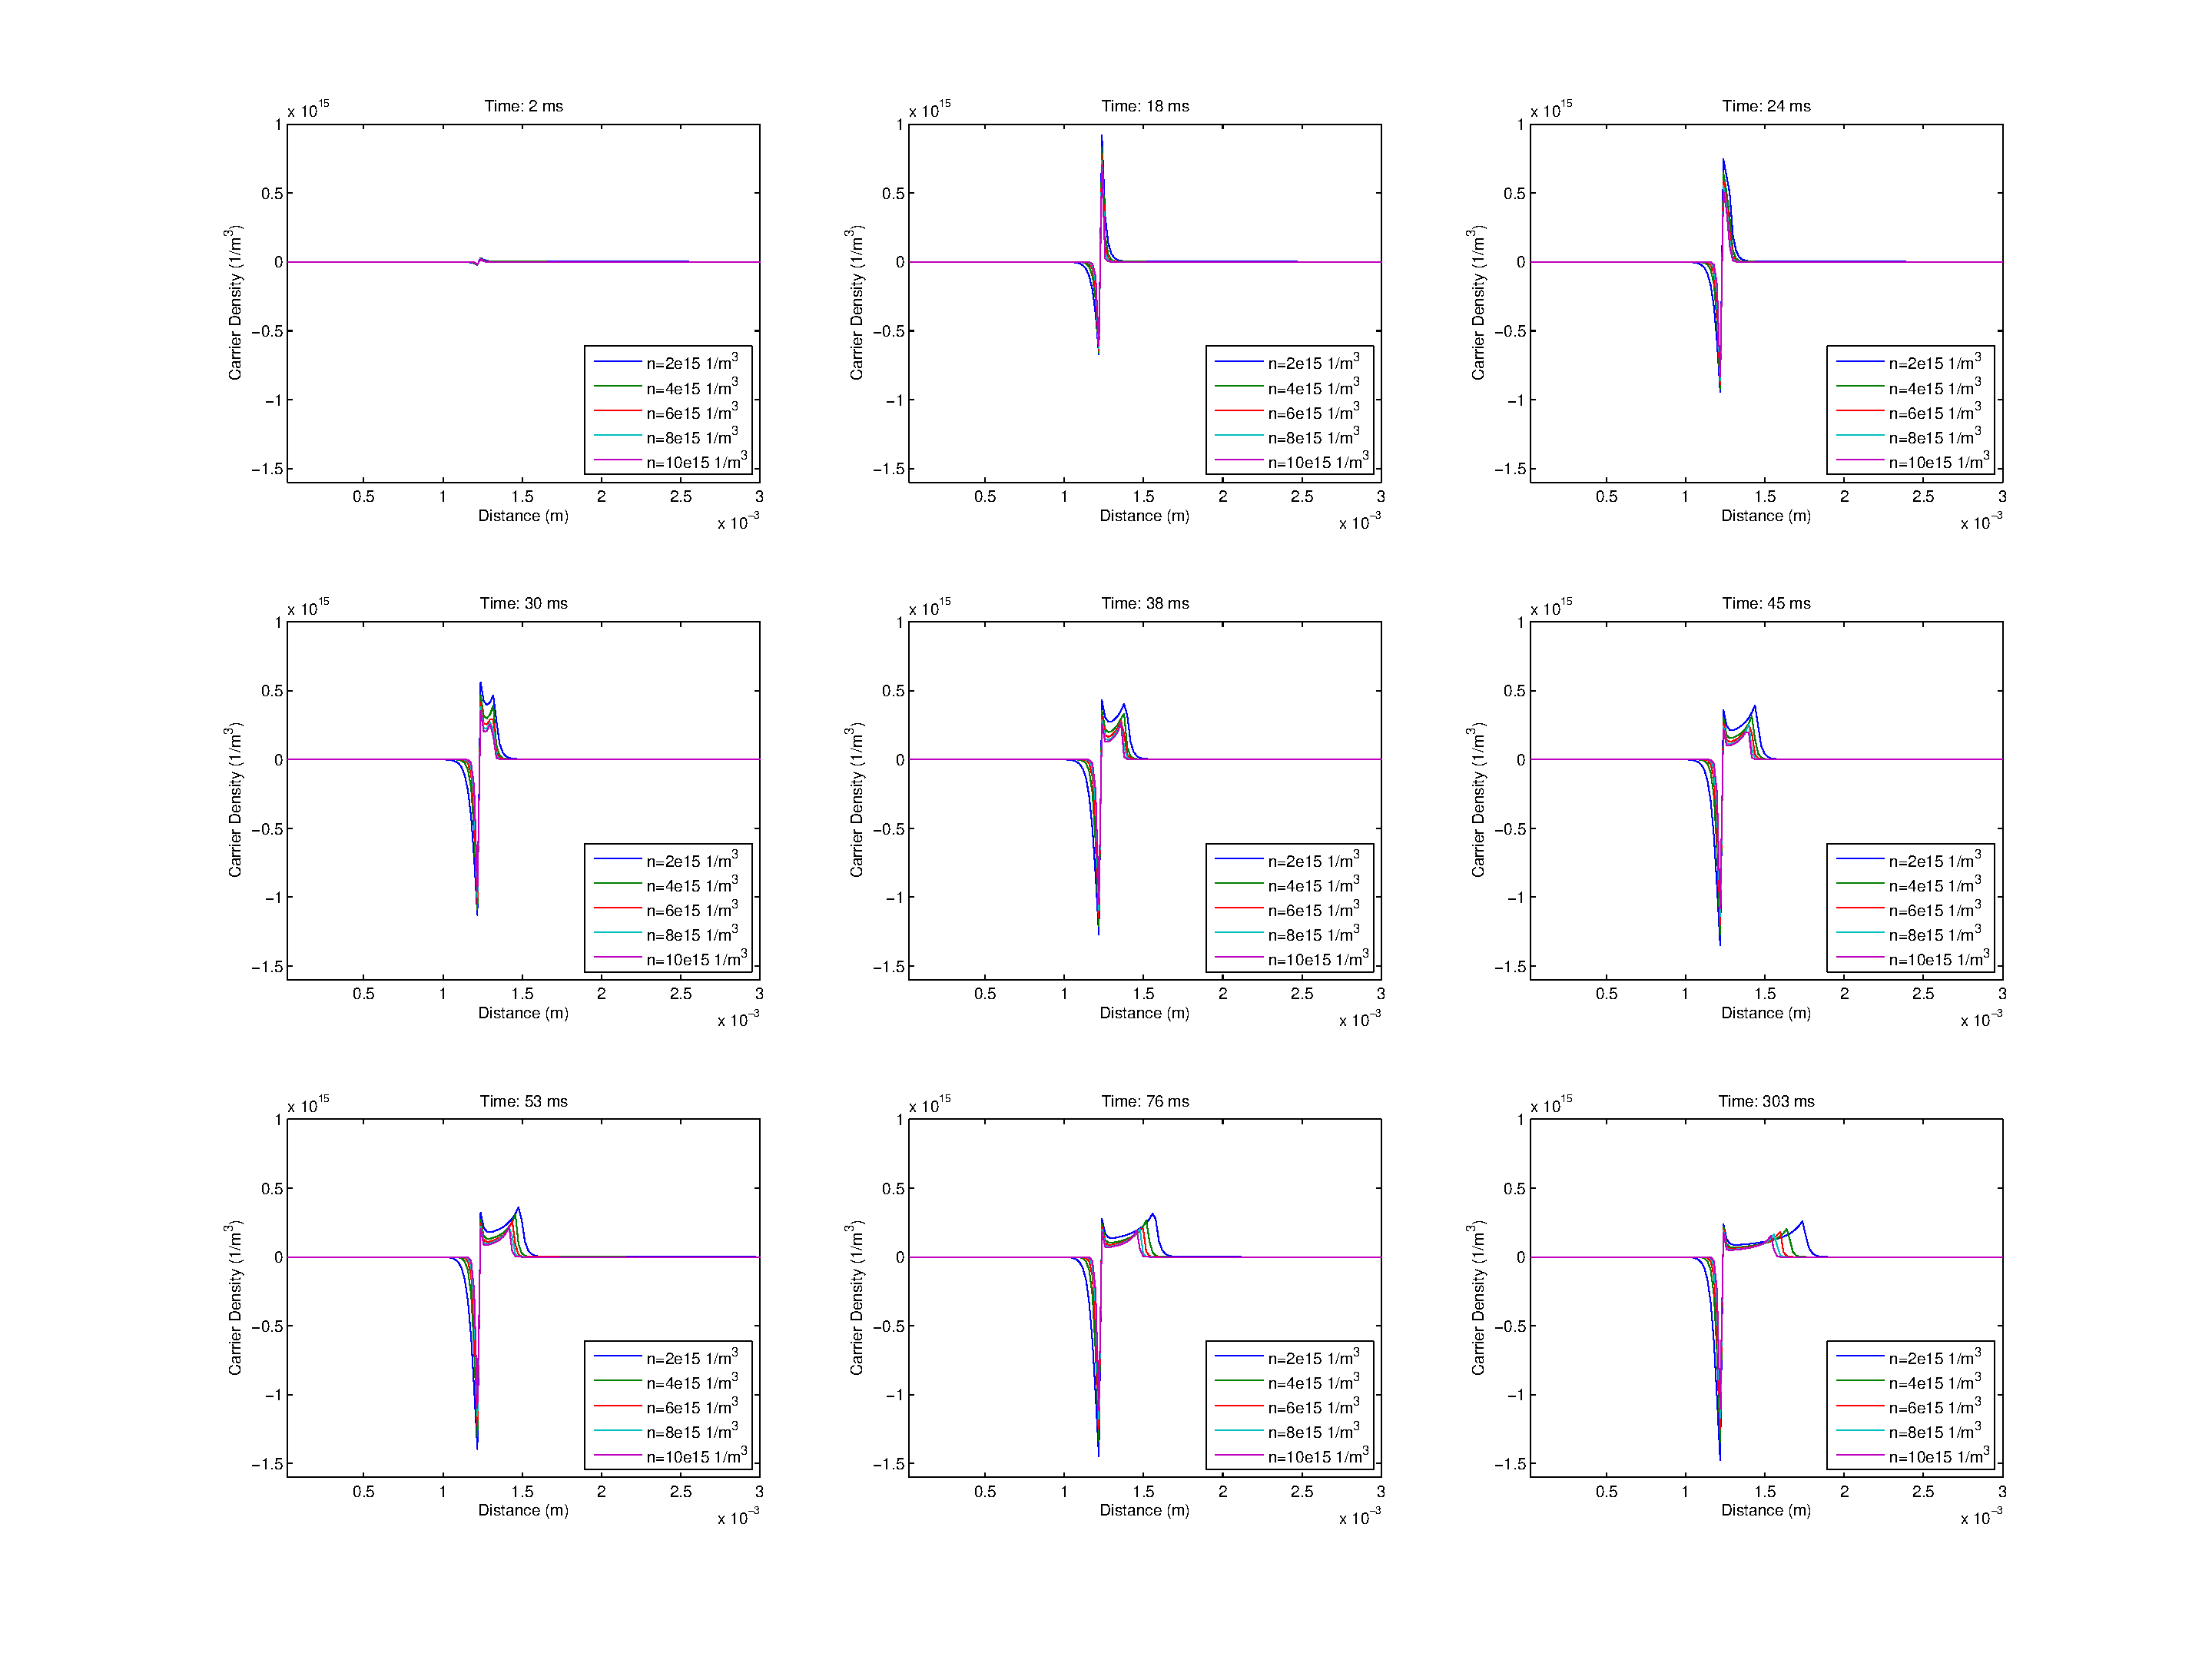
\includegraphics[scale=0.40]{Ex5NetQ_Time1}
\caption{} 
\label{}
\end{figure}
\end{landscape}

\begin{landscape}
\begin{figure}[!htp]
\centering
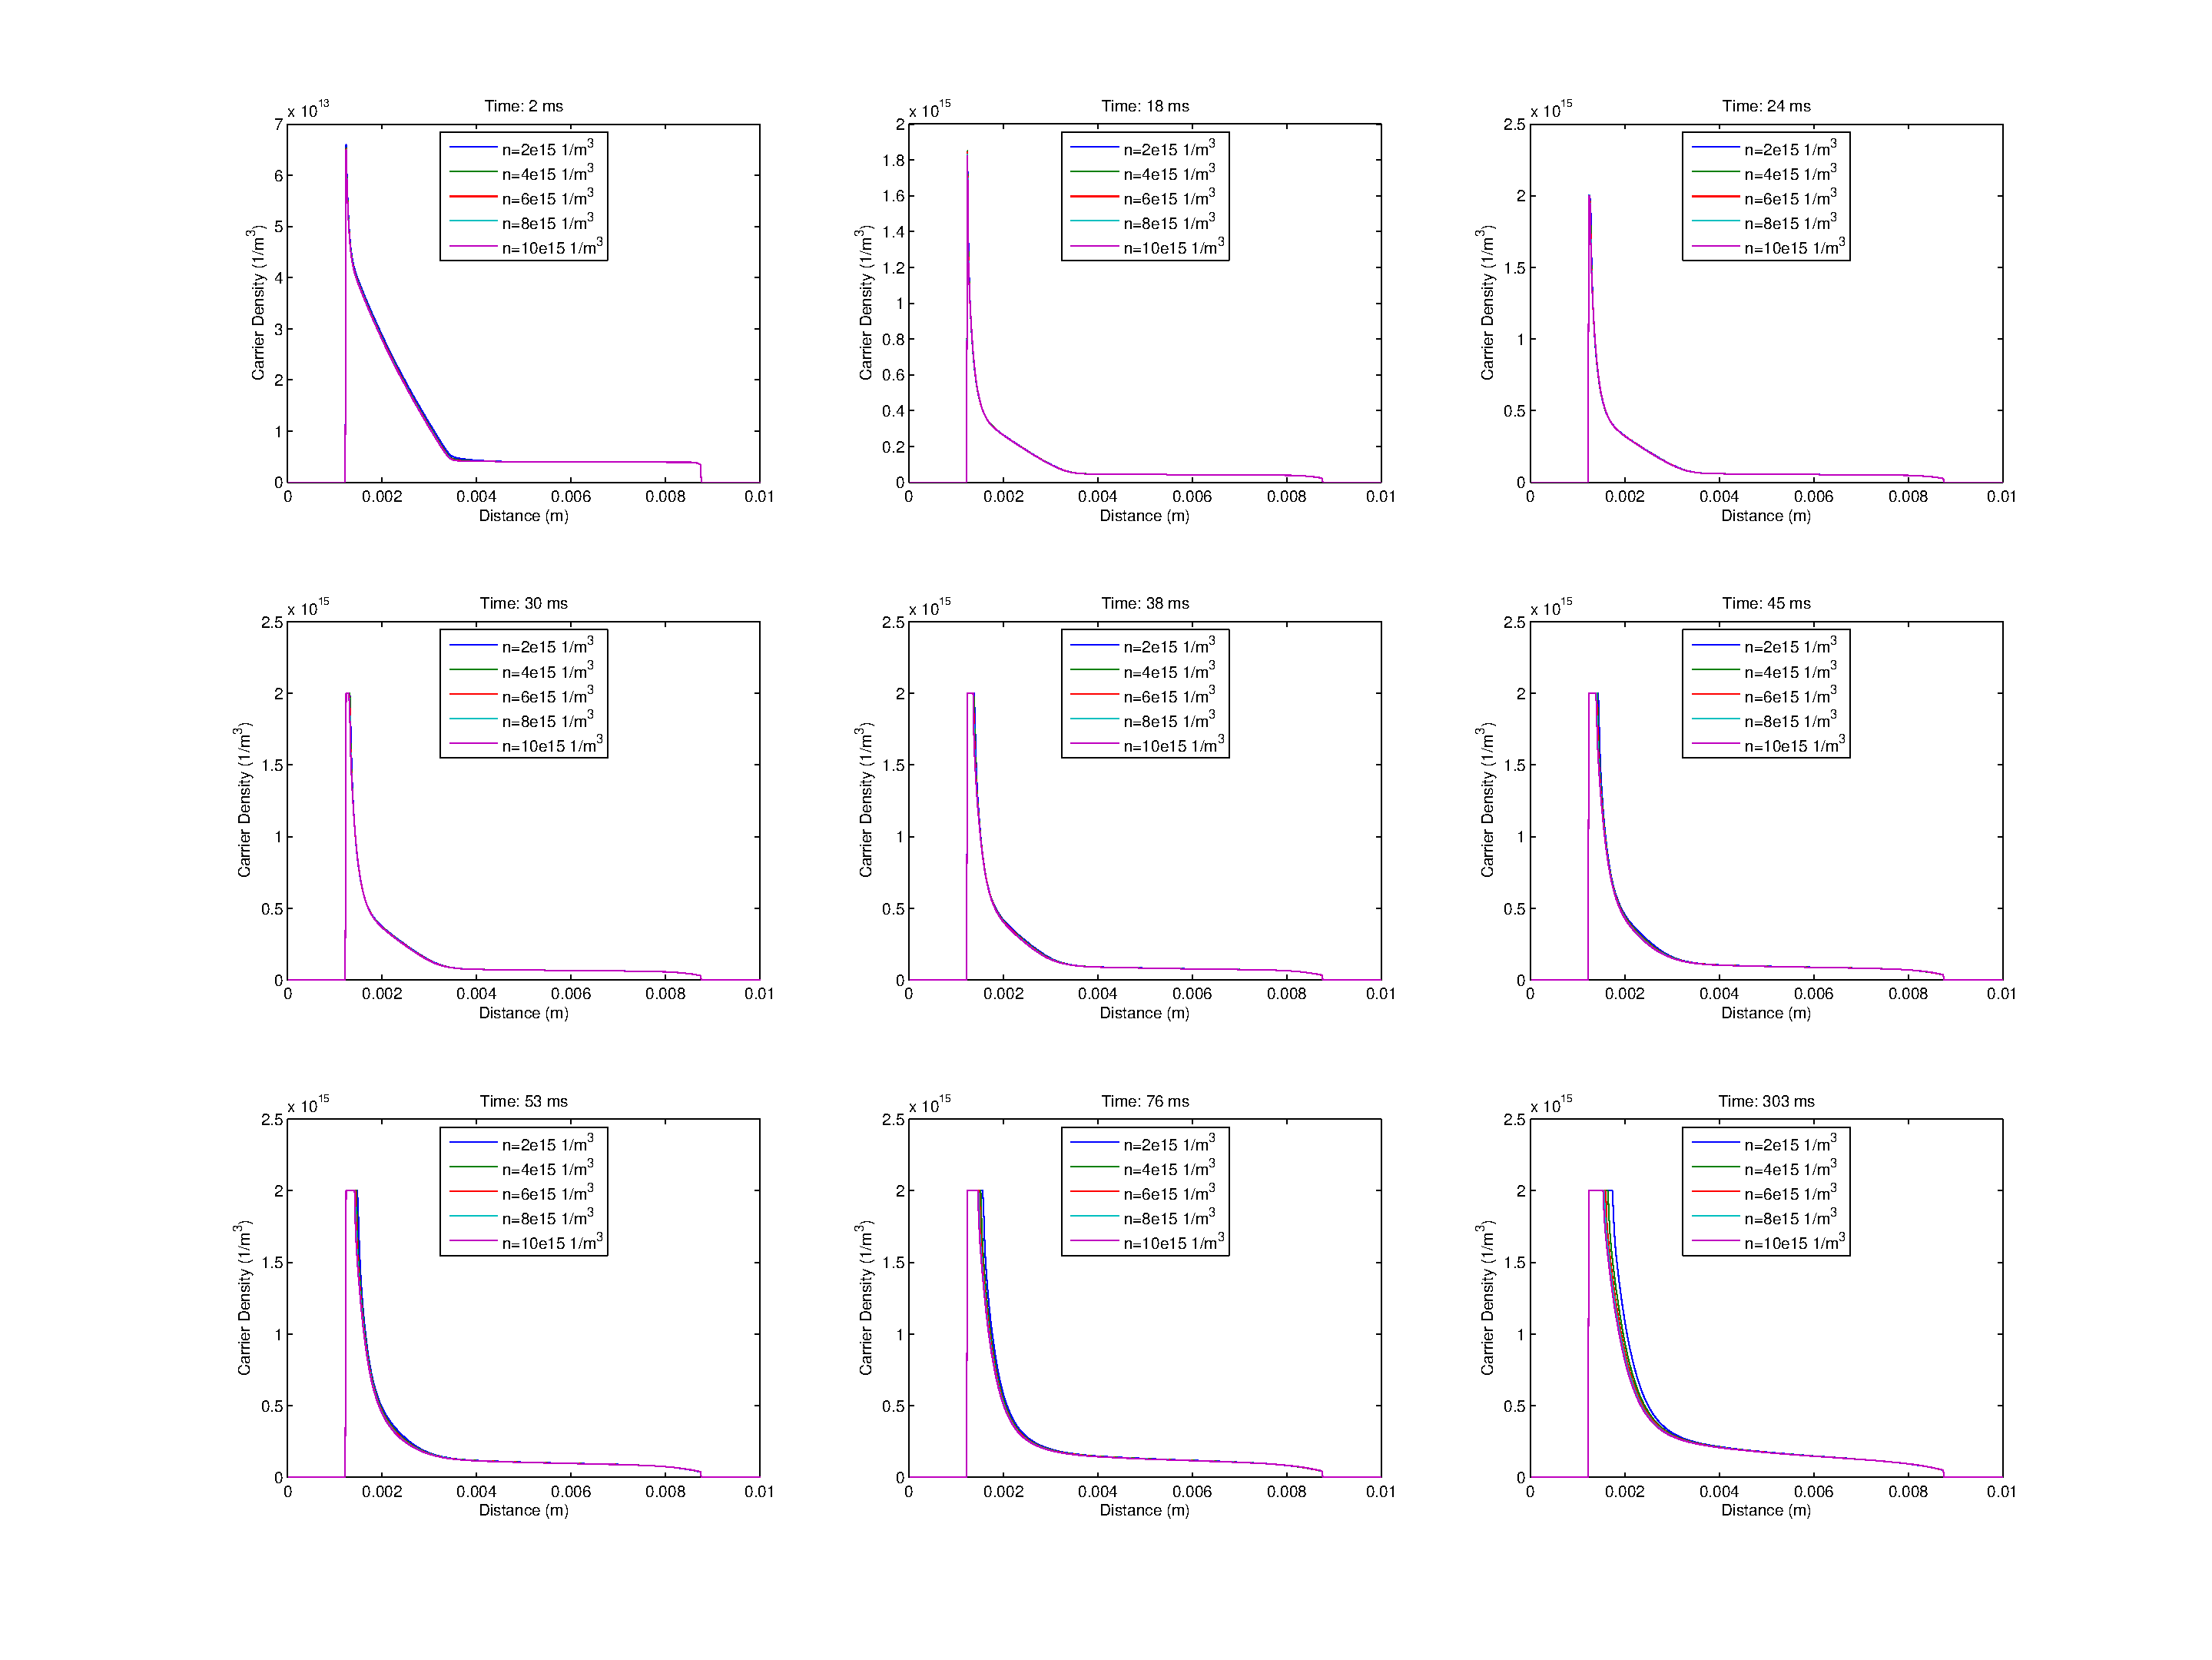
\includegraphics[scale=0.40]{Ex5Np_Time1}
\caption{} 
\label{}
\end{figure}
\end{landscape}

\begin{landscape}
\begin{figure}[!htp]
\centering
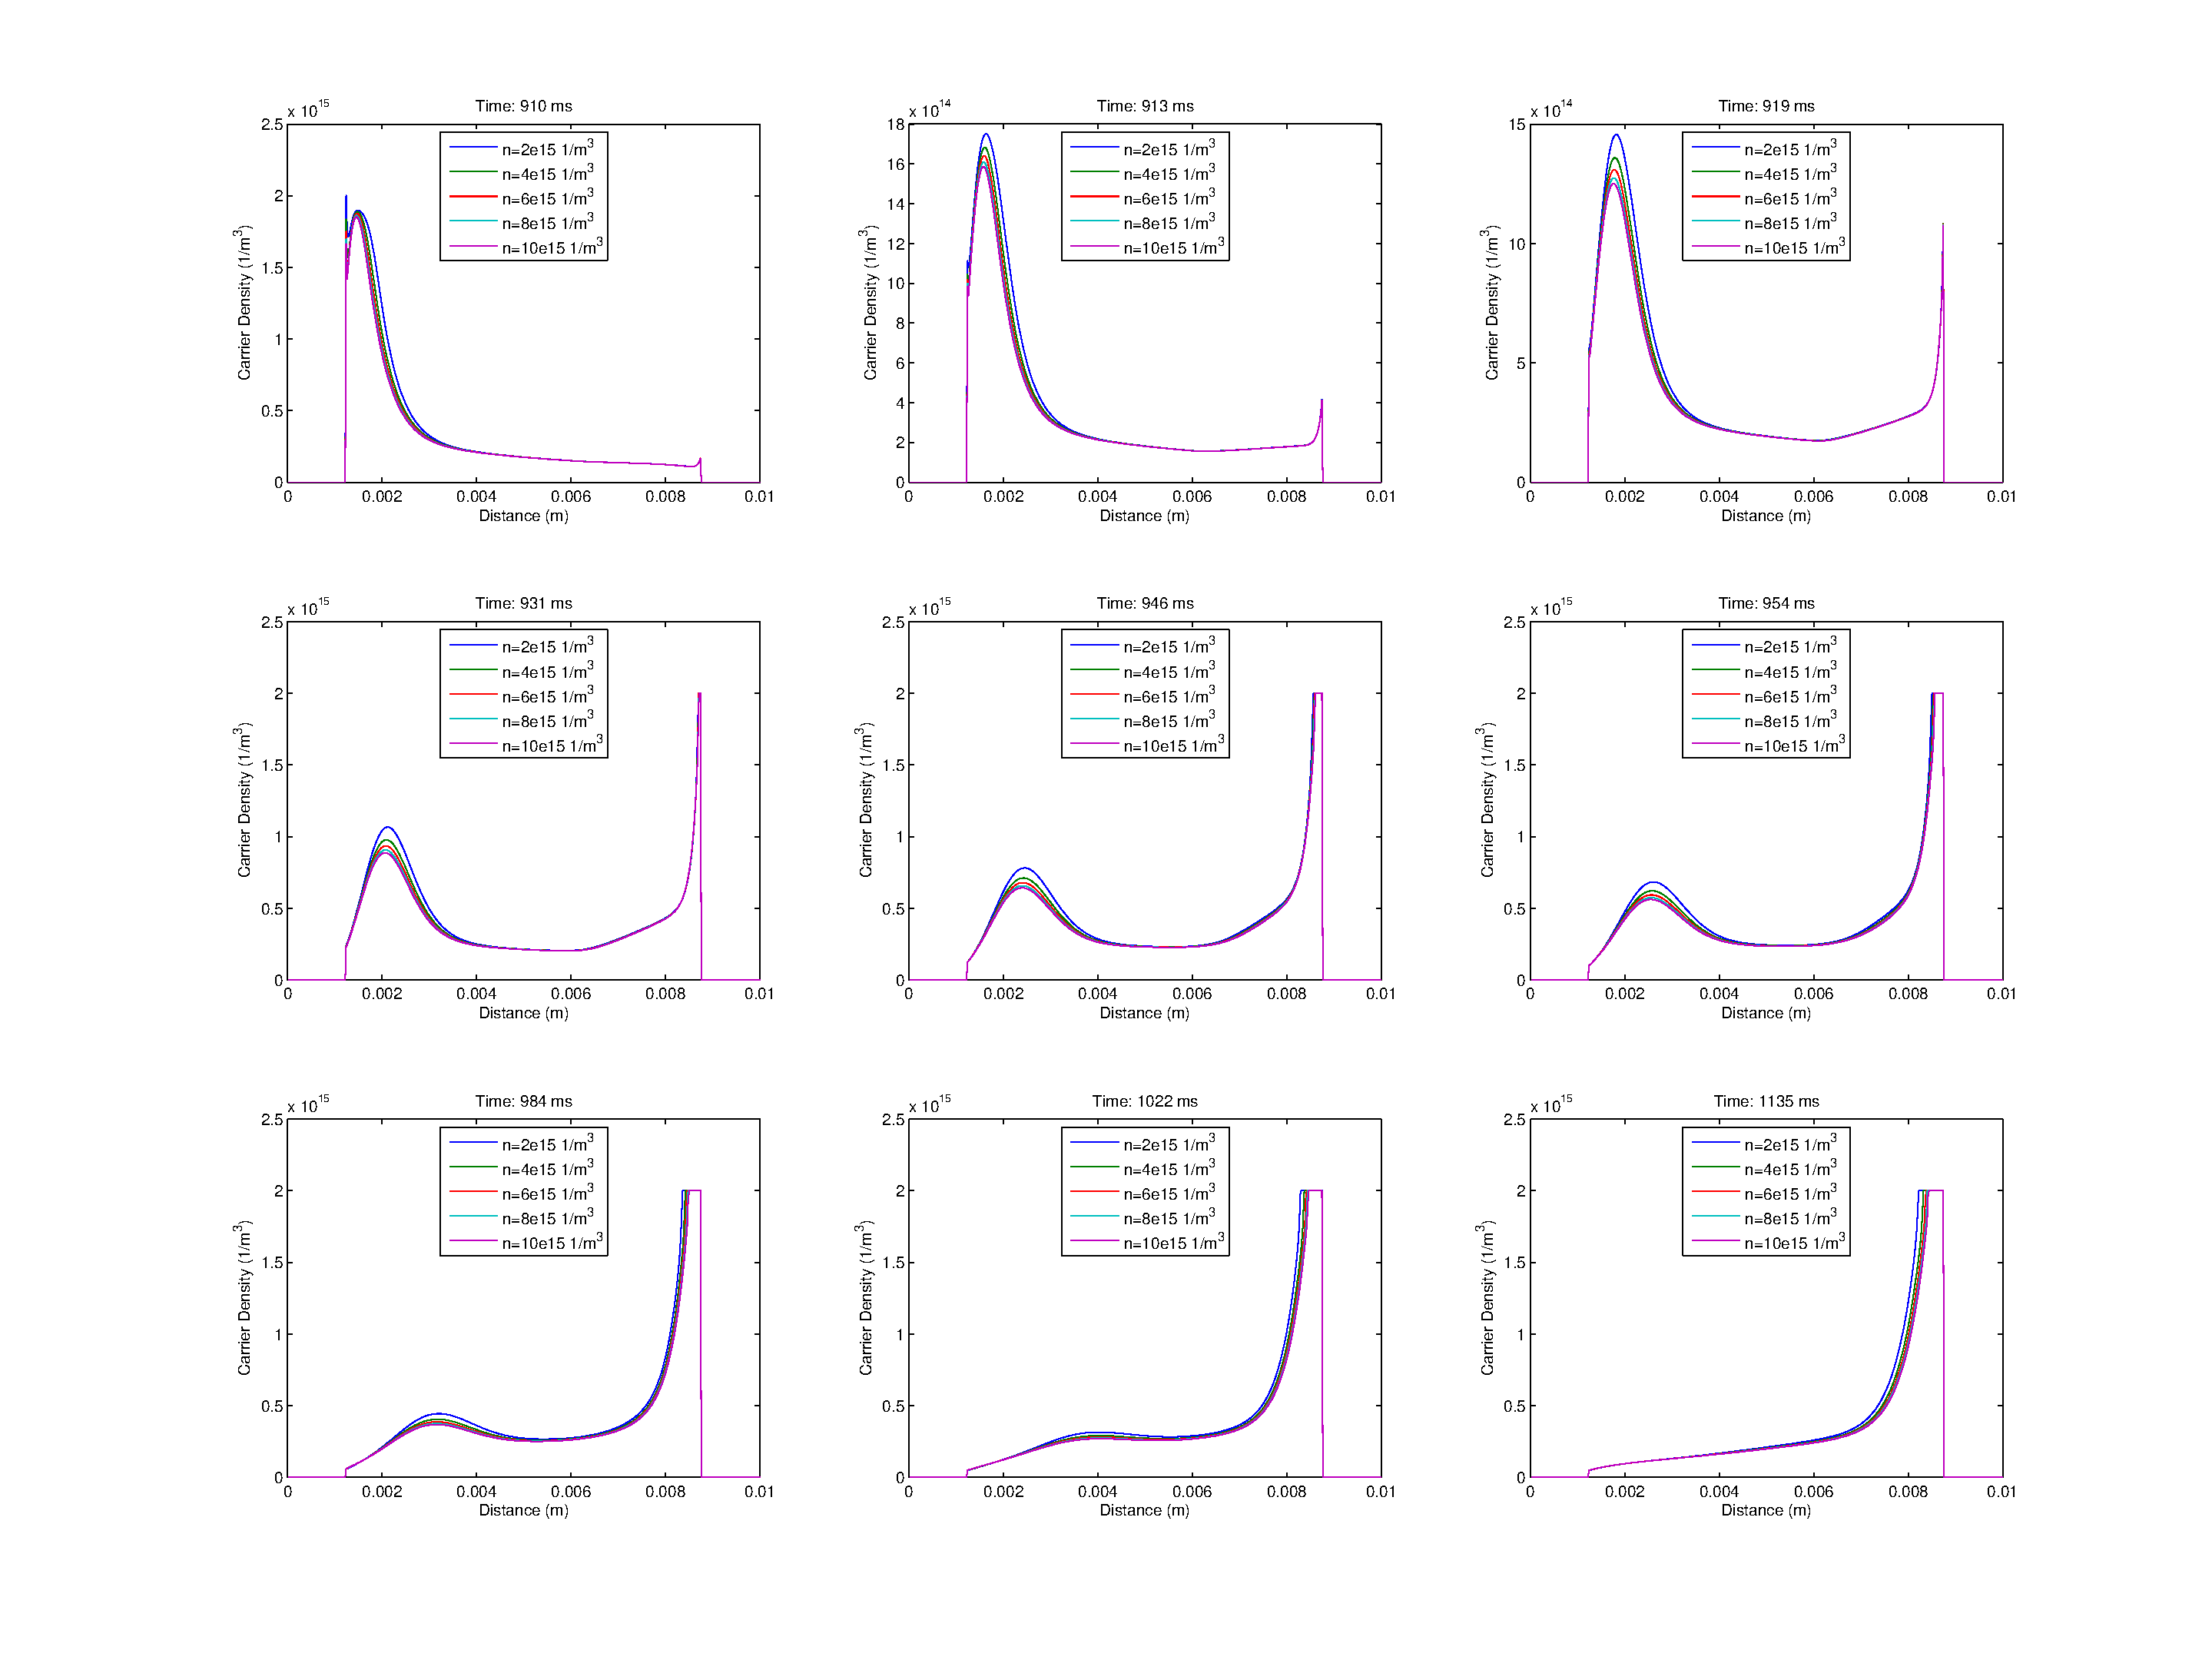
\includegraphics[scale=0.40]{Ex5Np_Time2}
\caption{} 
\label{}
\end{figure}
\end{landscape}

\begin{landscape}
\begin{figure}[!htp]
\centering
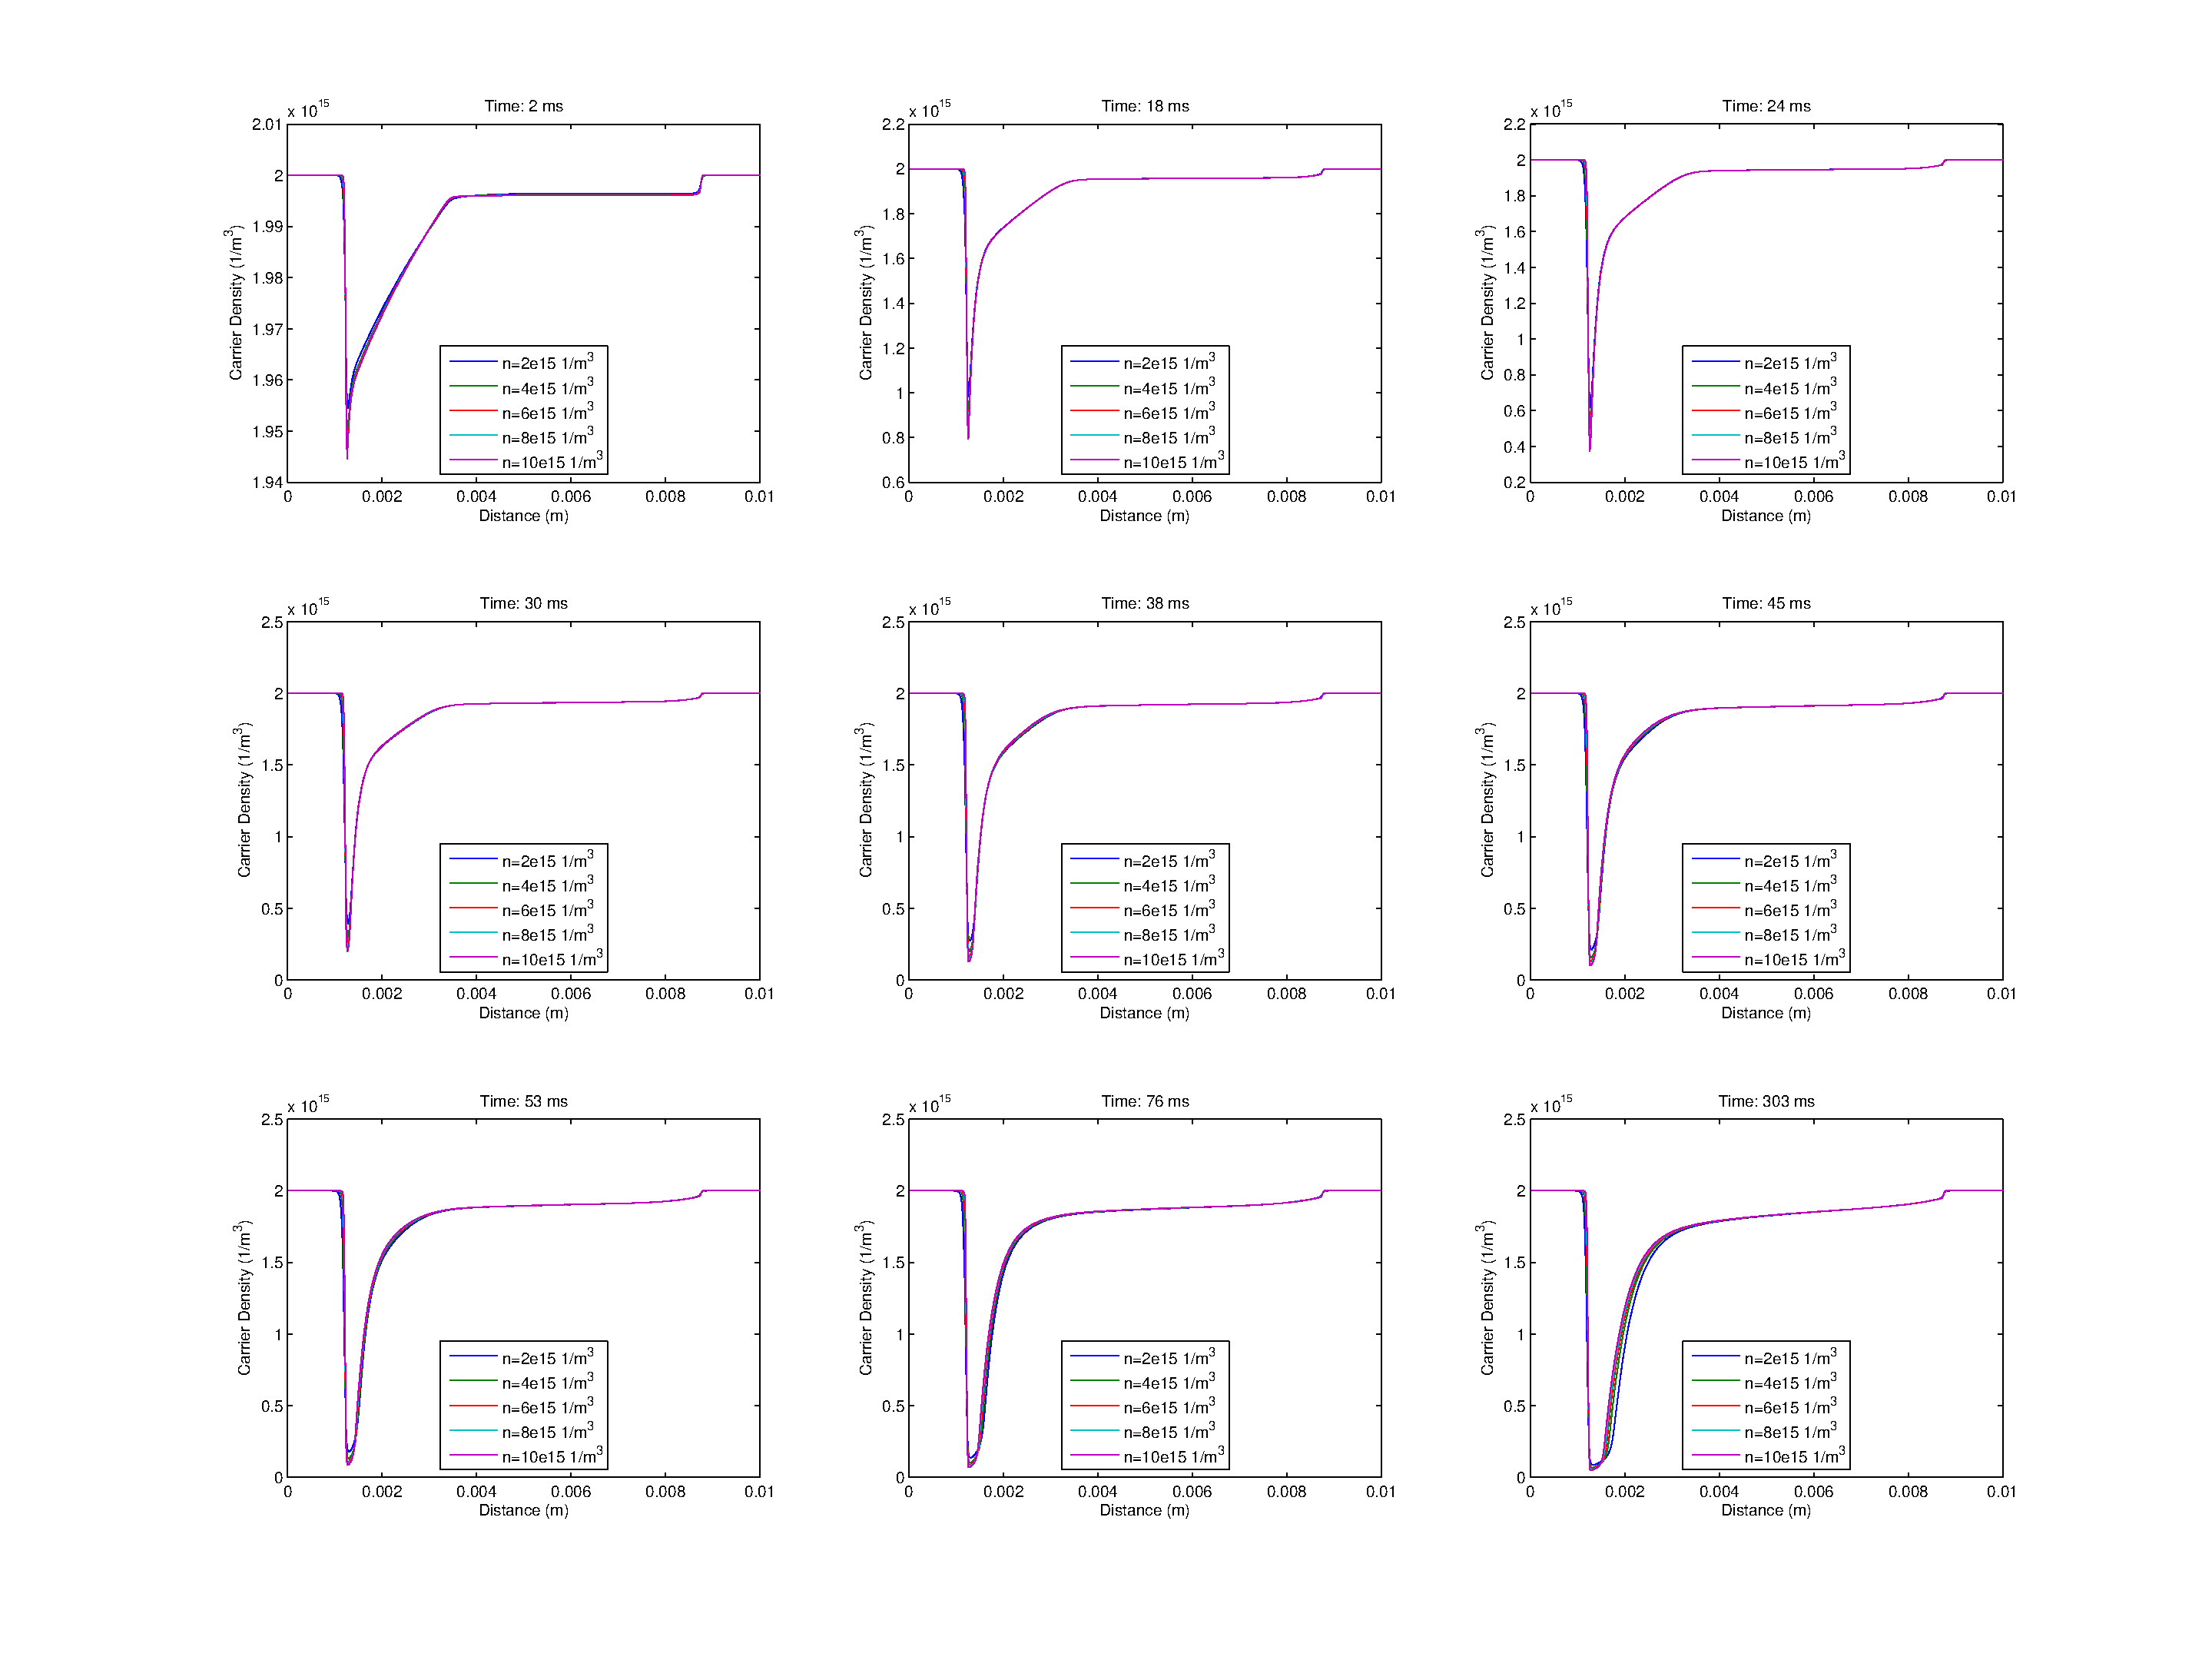
\includegraphics[scale=0.40]{Ex5p_Time1}
\caption{} 
\label{}
\end{figure}
\end{landscape}

\begin{landscape}
\begin{figure}[!htp]
\centering
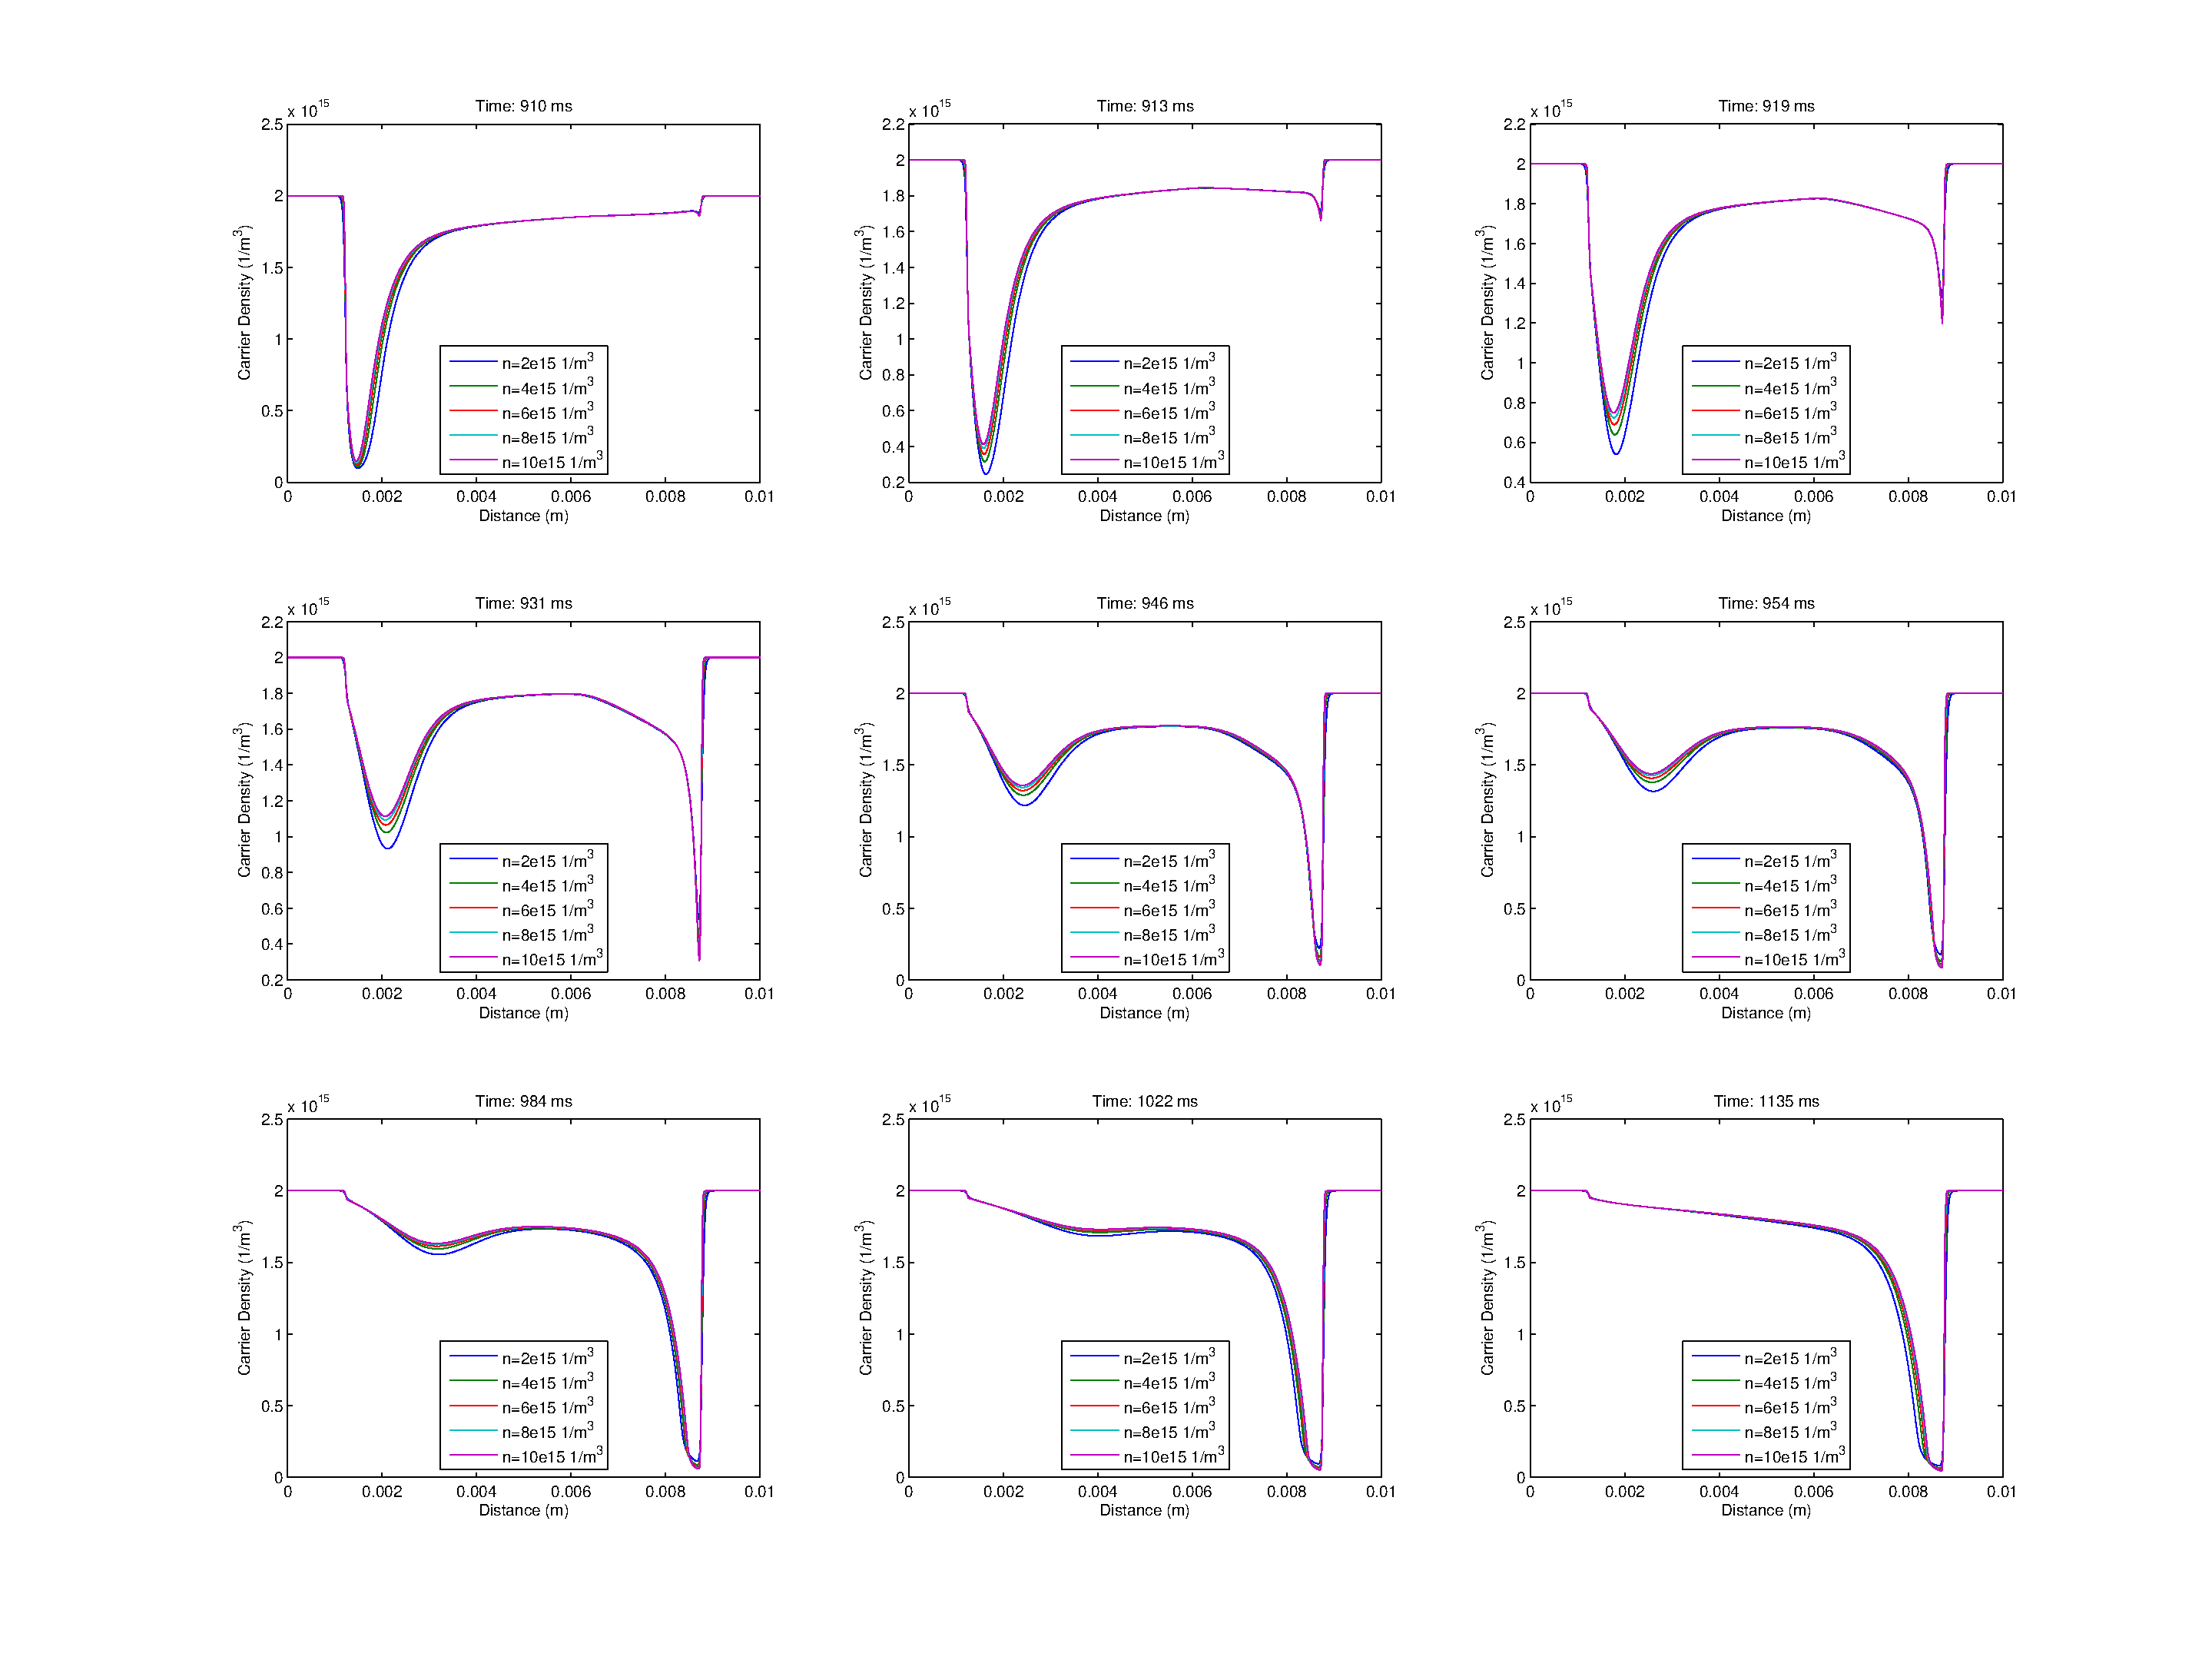
\includegraphics[scale=0.40]{Ex5p_Time2}
\caption{} 
\label{}
\end{figure}
\end{landscape}


\begin{landscape}
\begin{figure}[!htp]
\centering
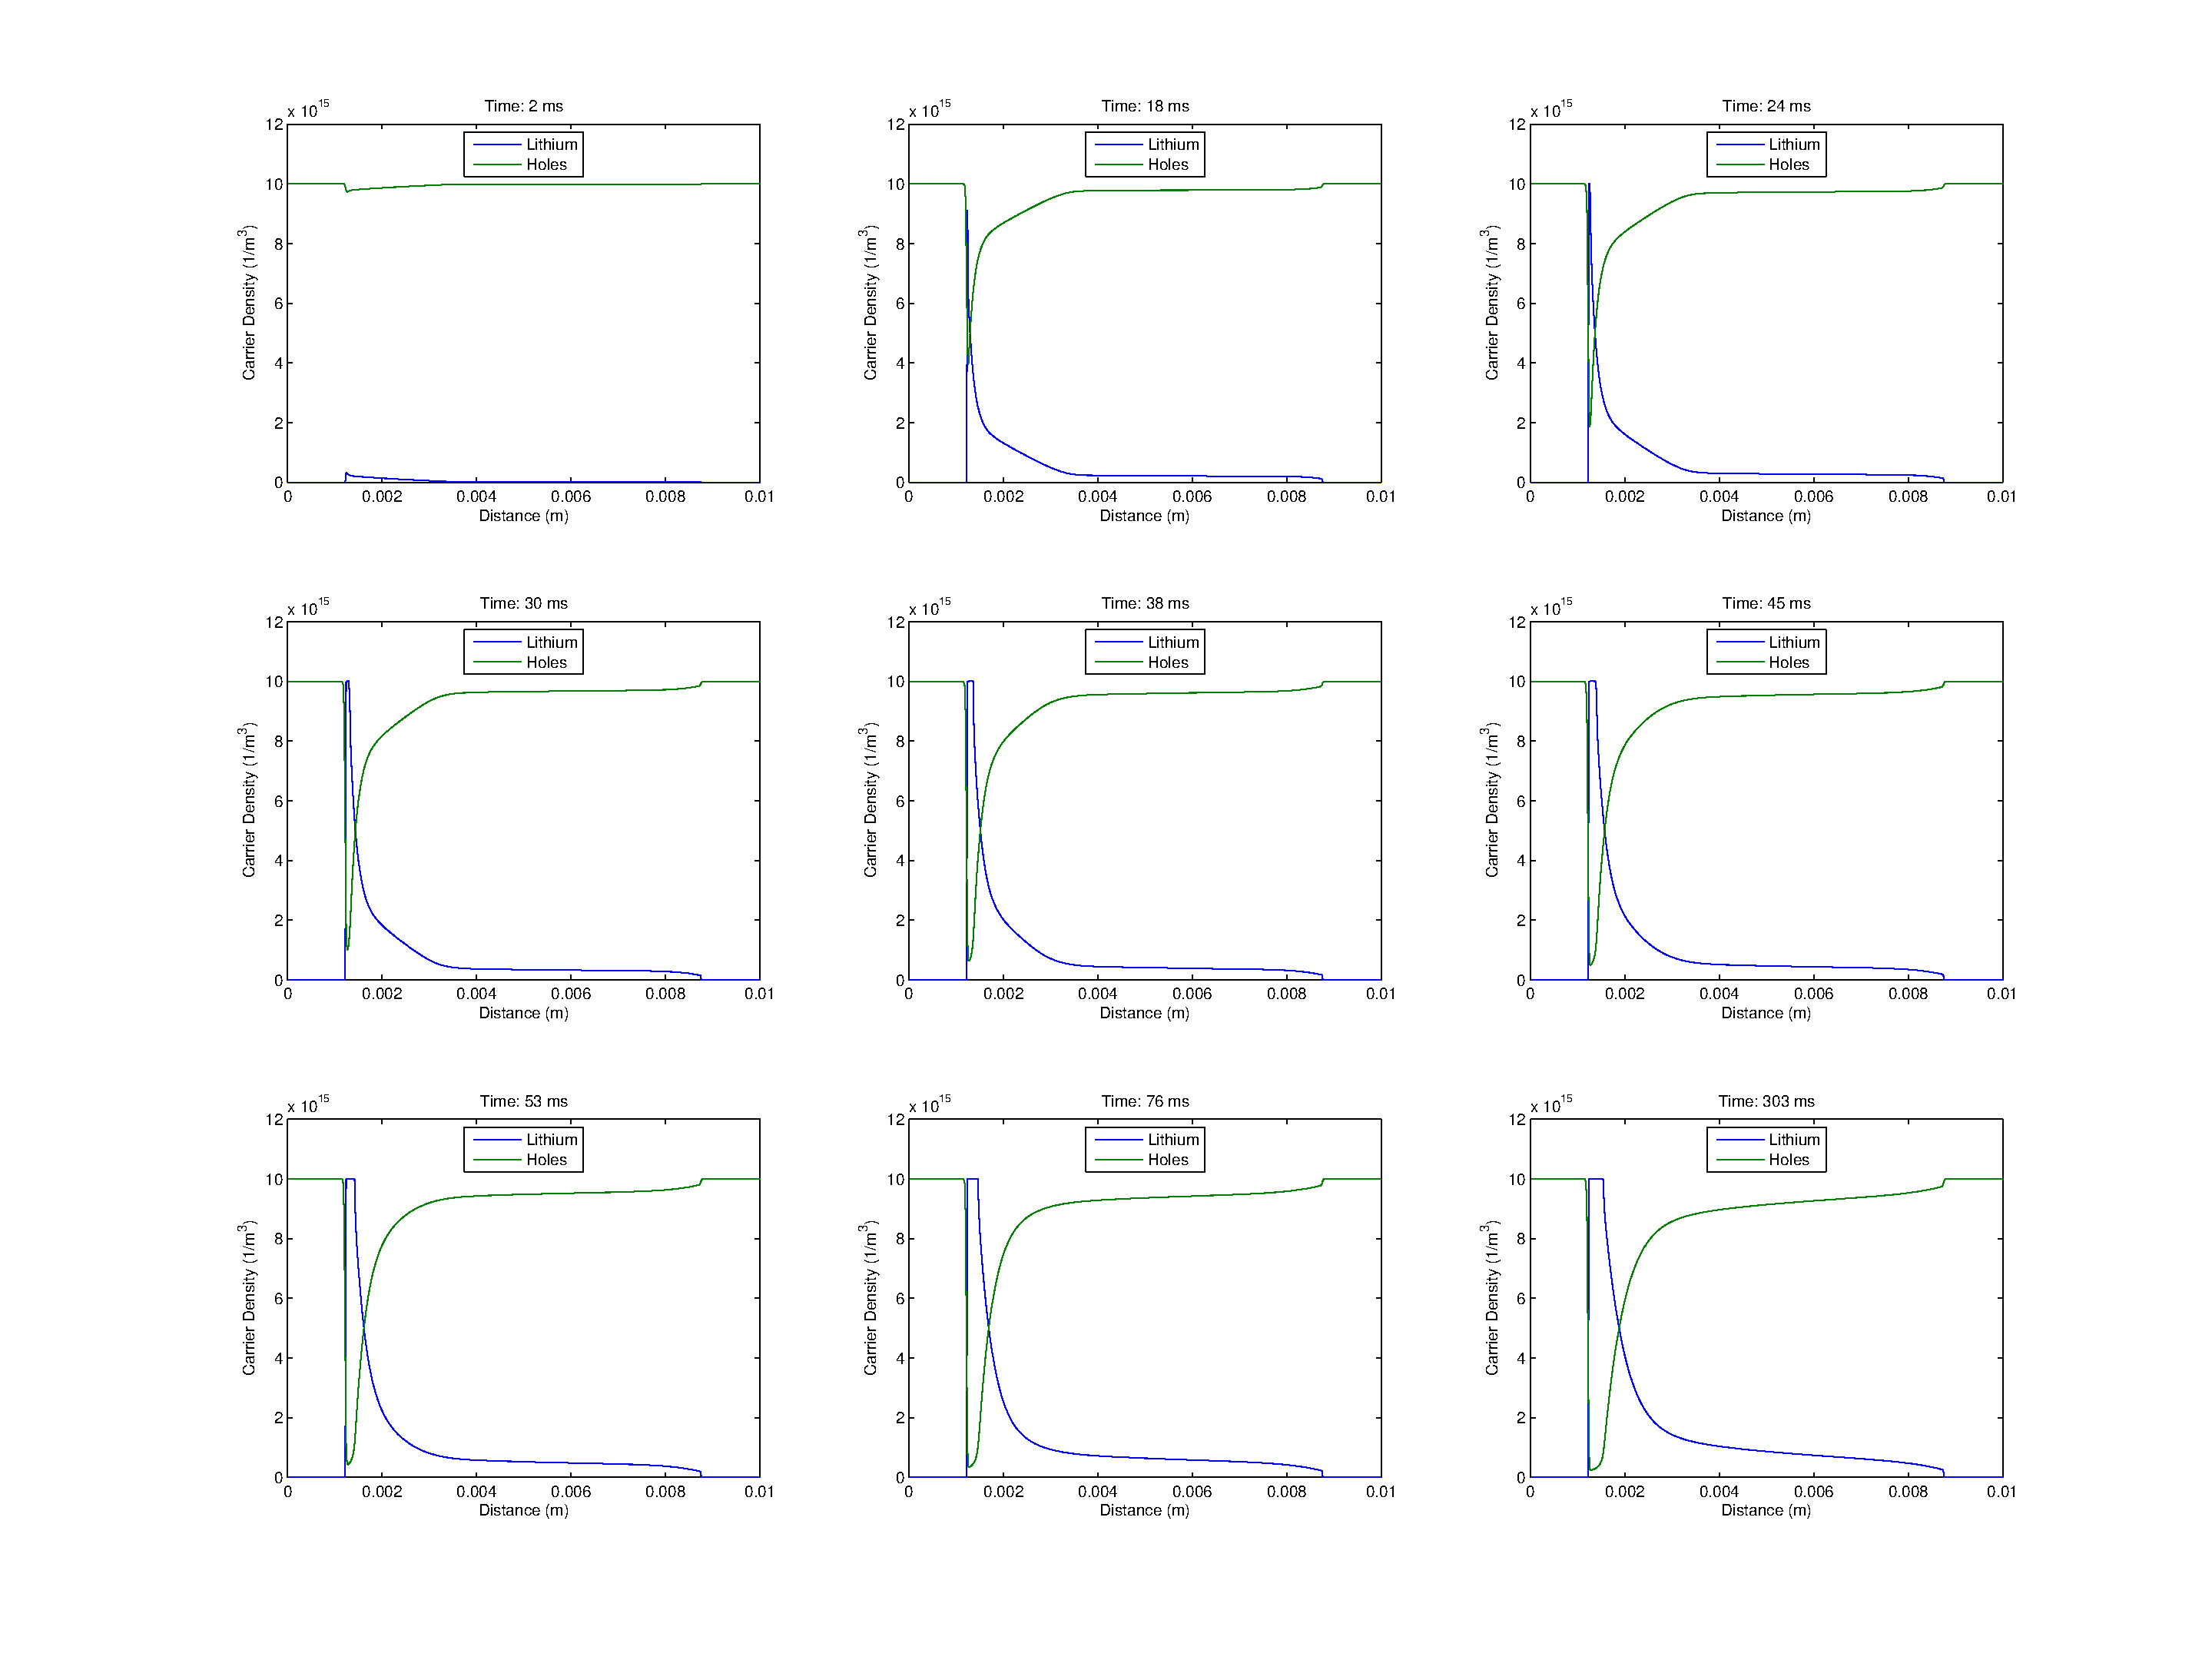
\includegraphics[scale=0.40]{Ex5pNp_Time1}
\caption{} 
\label{}
\end{figure}
\end{landscape}

\begin{landscape}
\begin{figure}[!htp]
\centering
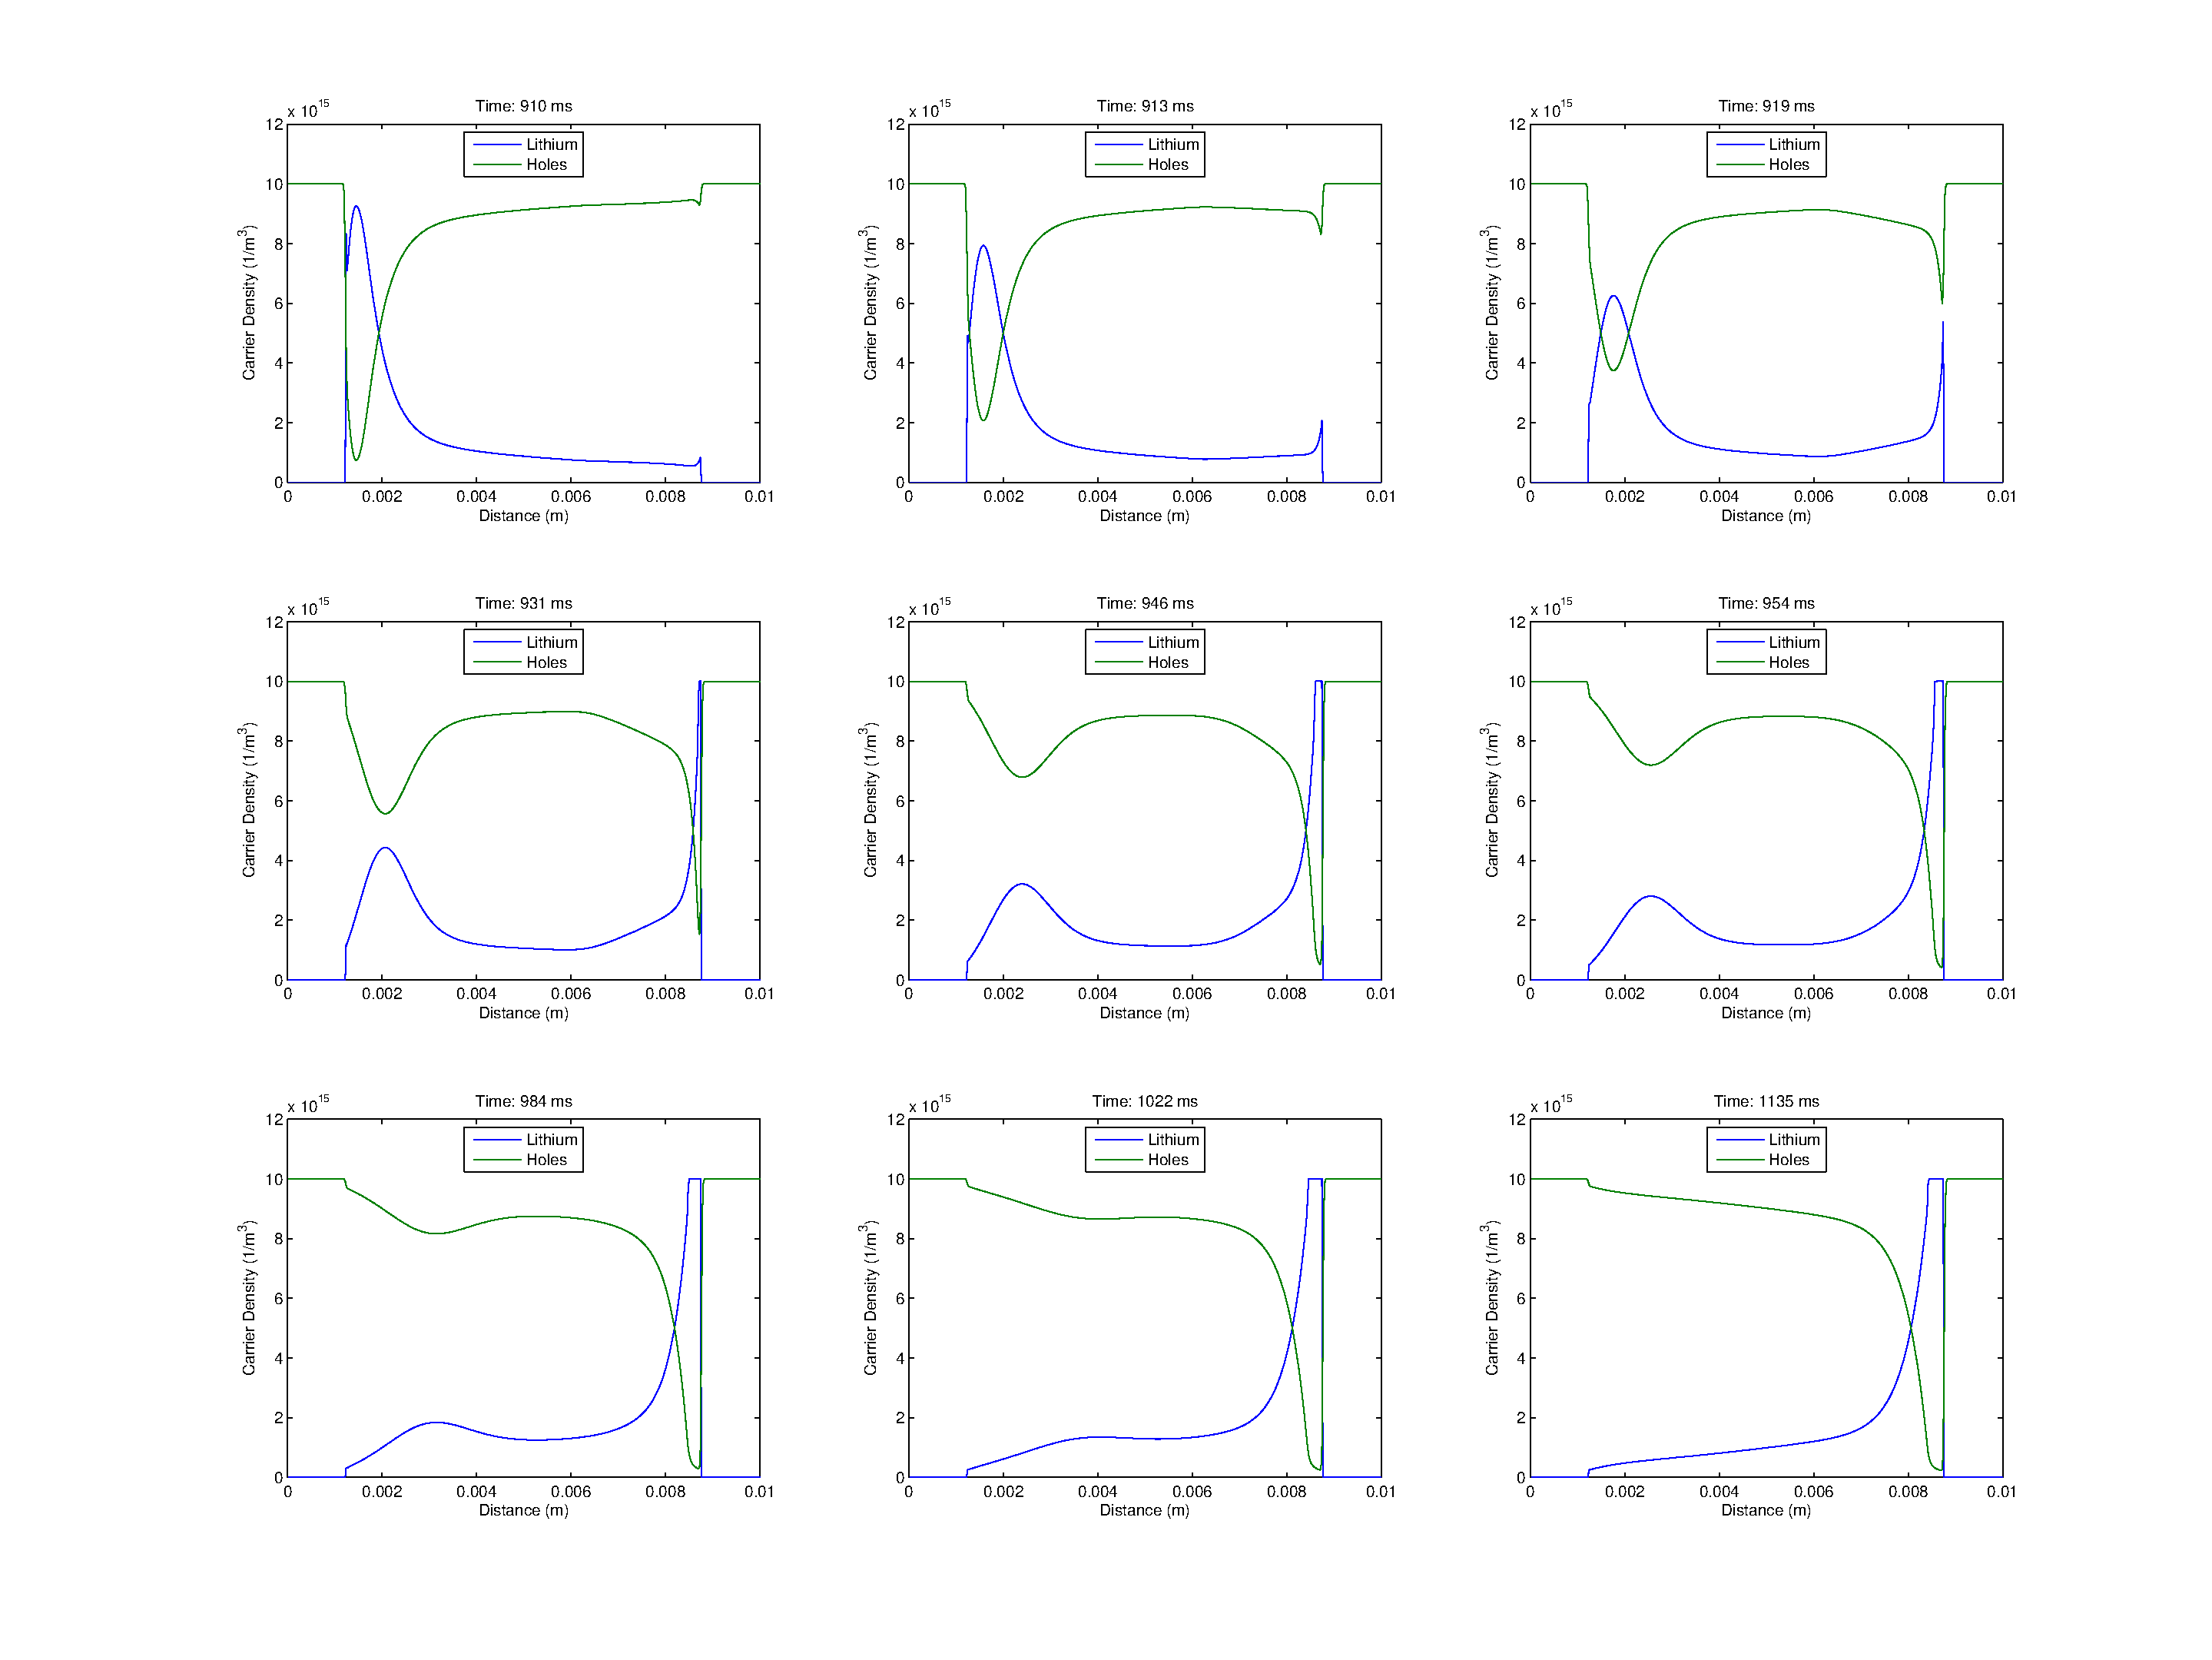
\includegraphics[scale=0.40]{Ex5pNp_Time2}
\caption{} 
\label{}
\end{figure}
\end{landscape}


\begin{figure}[!htp]
\centering
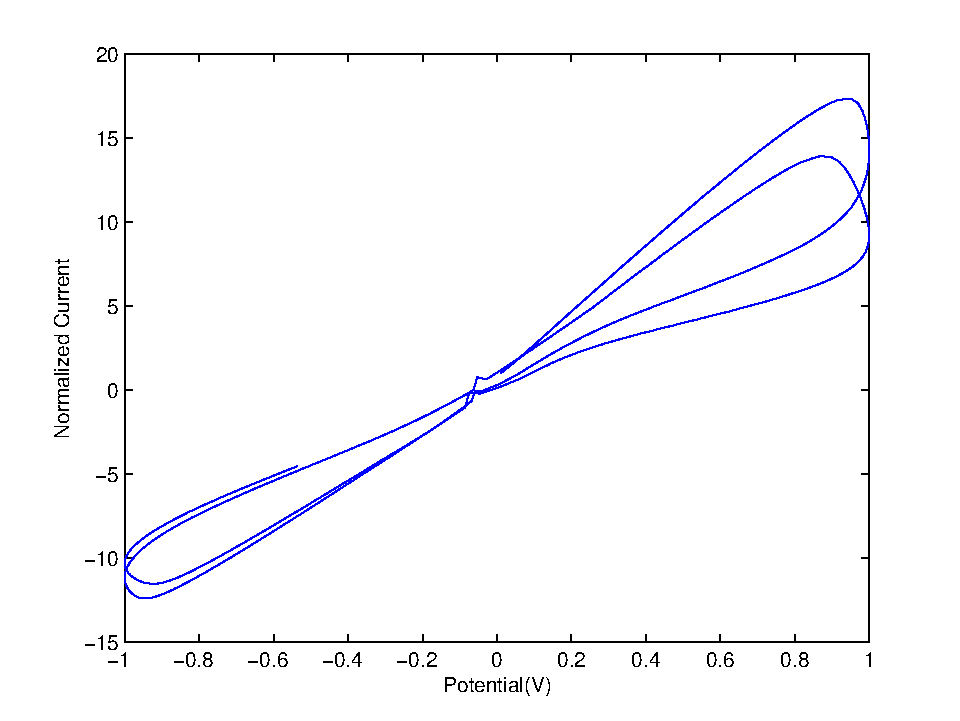
\includegraphics[scale=0.60]{Ex5Bowtie}
\caption{} 
\label{}
\end{figure}

\begin{figure}[!htp]
\centering
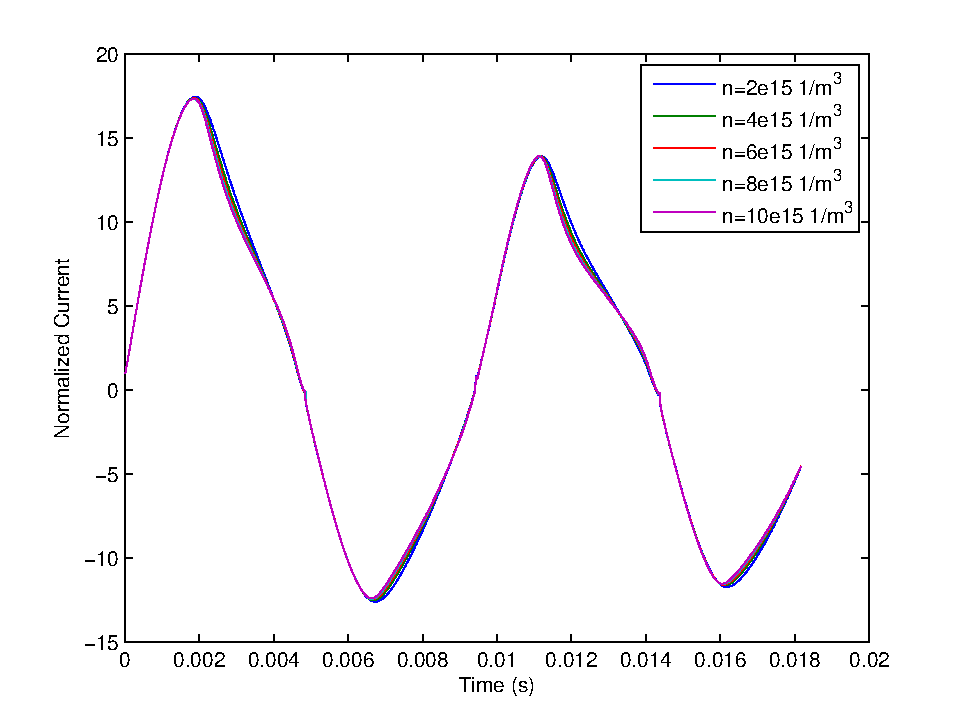
\includegraphics[scale=0.60]{Ex5Current}
\caption{} 
\label{}
\end{figure}



\clearpage
\subsection{PEDOT:PSS with Notch (Cross Section 2)}
\begin{figure}[!htp]
\centering
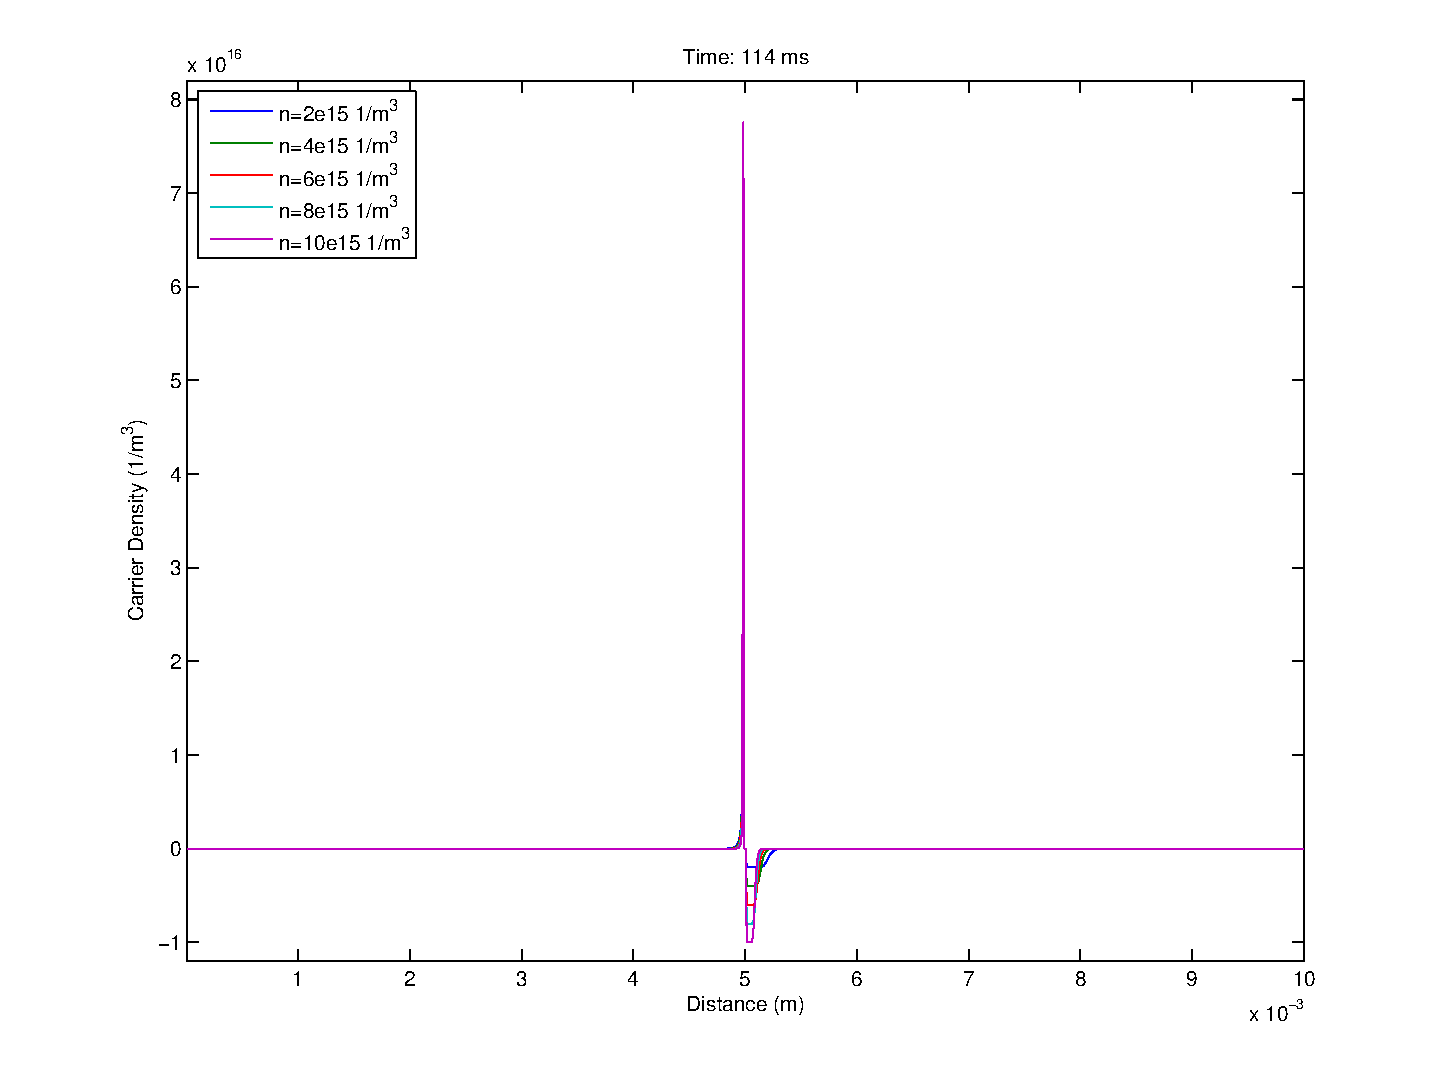
\includegraphics[scale=0.60]{Ex3NetQ_Time_All}
\caption{} 
\label{}
\end{figure}


\begin{landscape}
\begin{figure}[!htp]
\centering
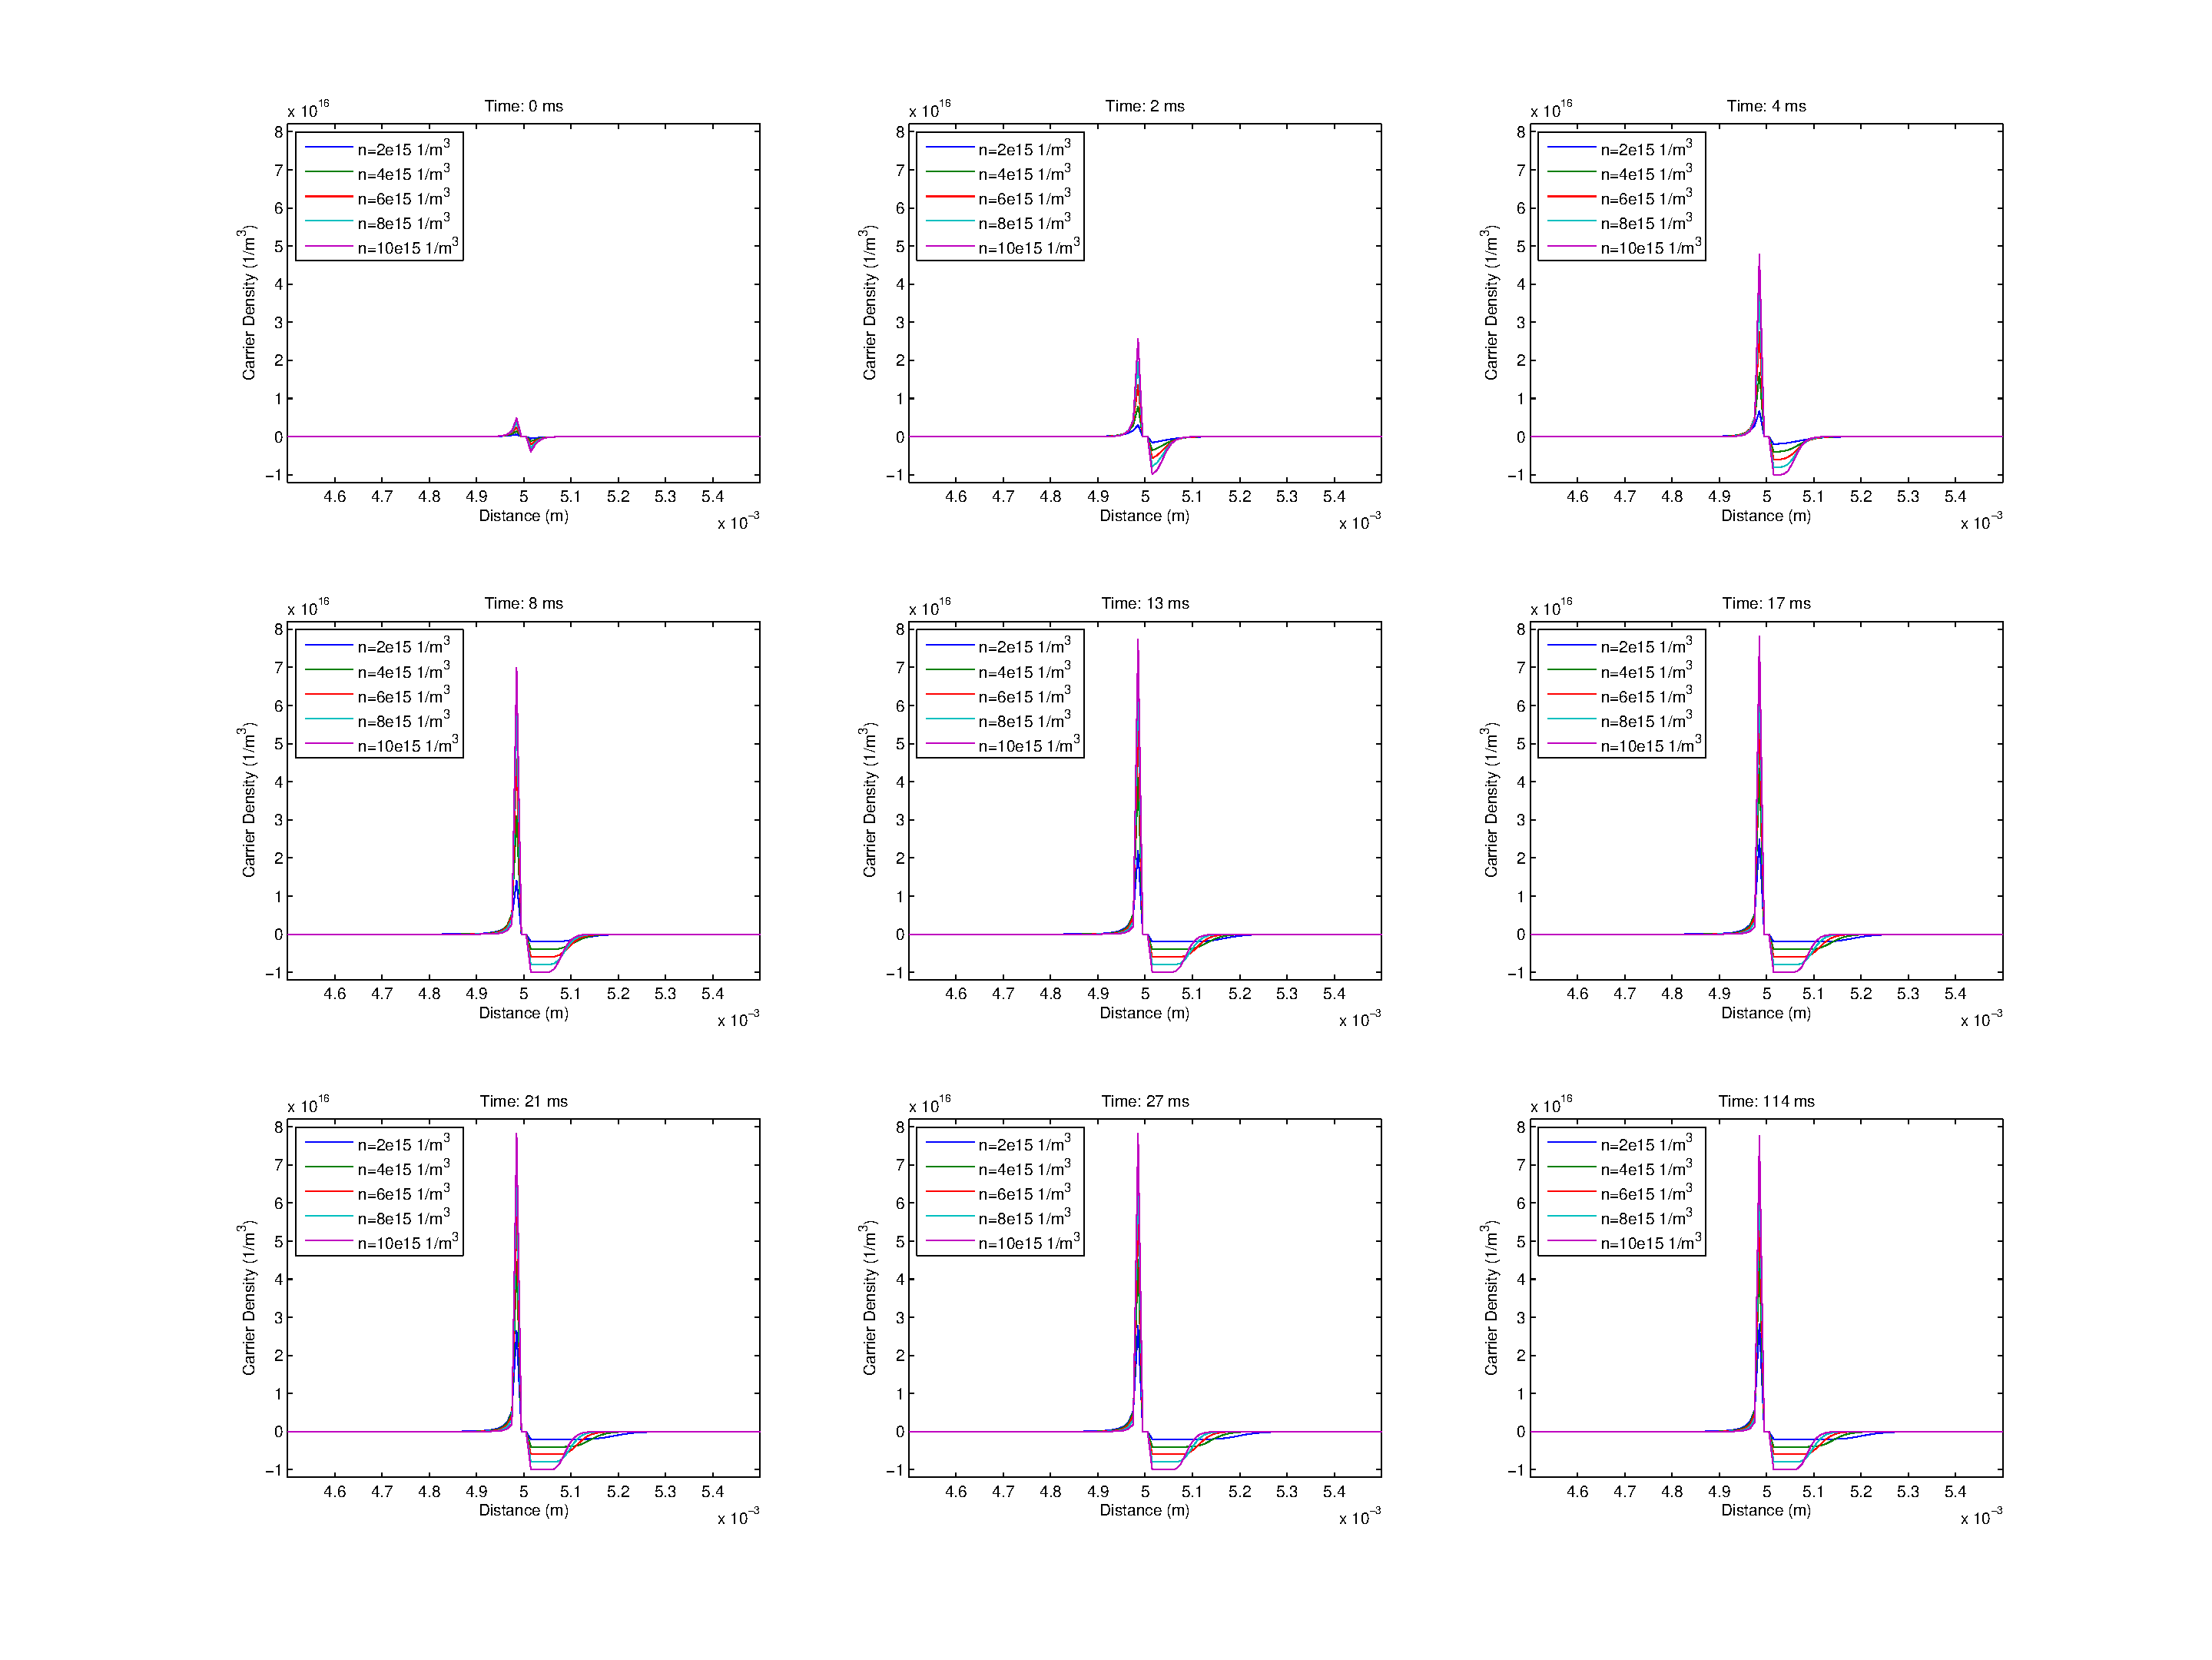
\includegraphics[scale=0.40]{Ex3NetQ_Time}
\caption{} 
\label{}
\end{figure}
\end{landscape}

\begin{landscape}
\begin{figure}[!htp]
\centering
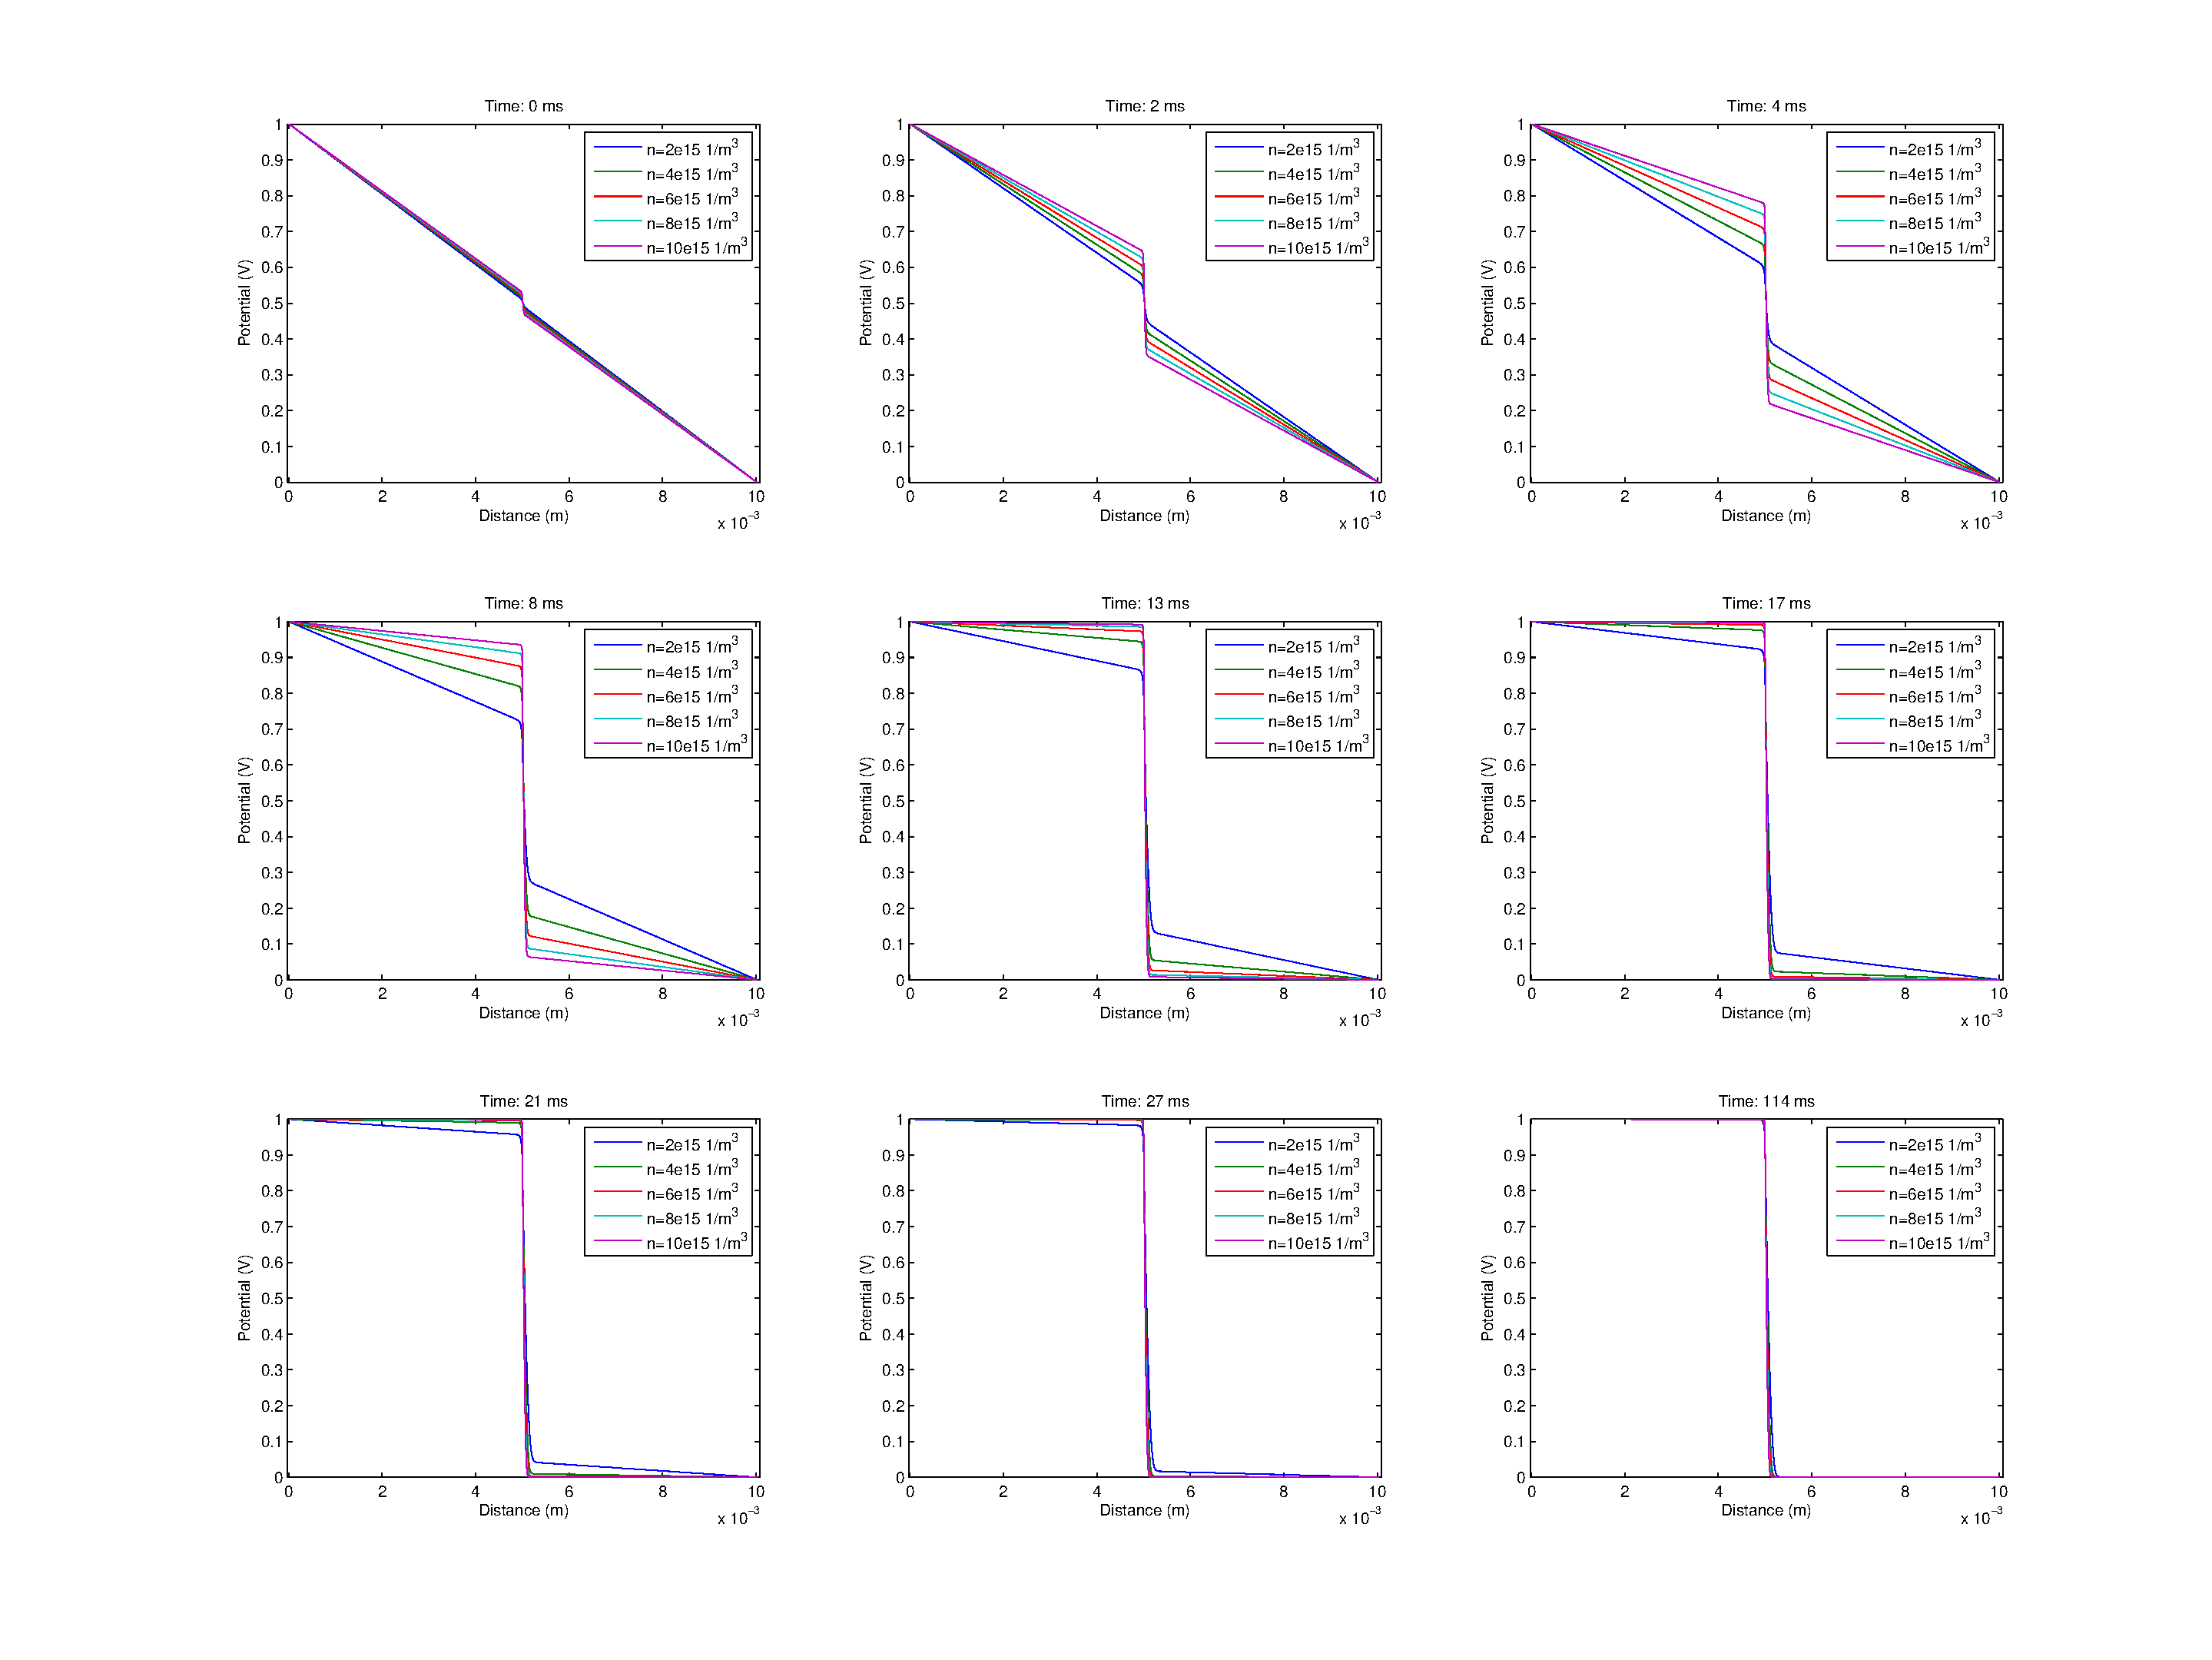
\includegraphics[scale=0.40]{Ex3V_Time}
\caption{} 
\label{}
\end{figure}
\end{landscape}

\clearpage
\subsection{Electrolyte/PEDOT Interface (Cross Section 3) }


\begin{landscape}
\begin{figure}[!htp]
\centering
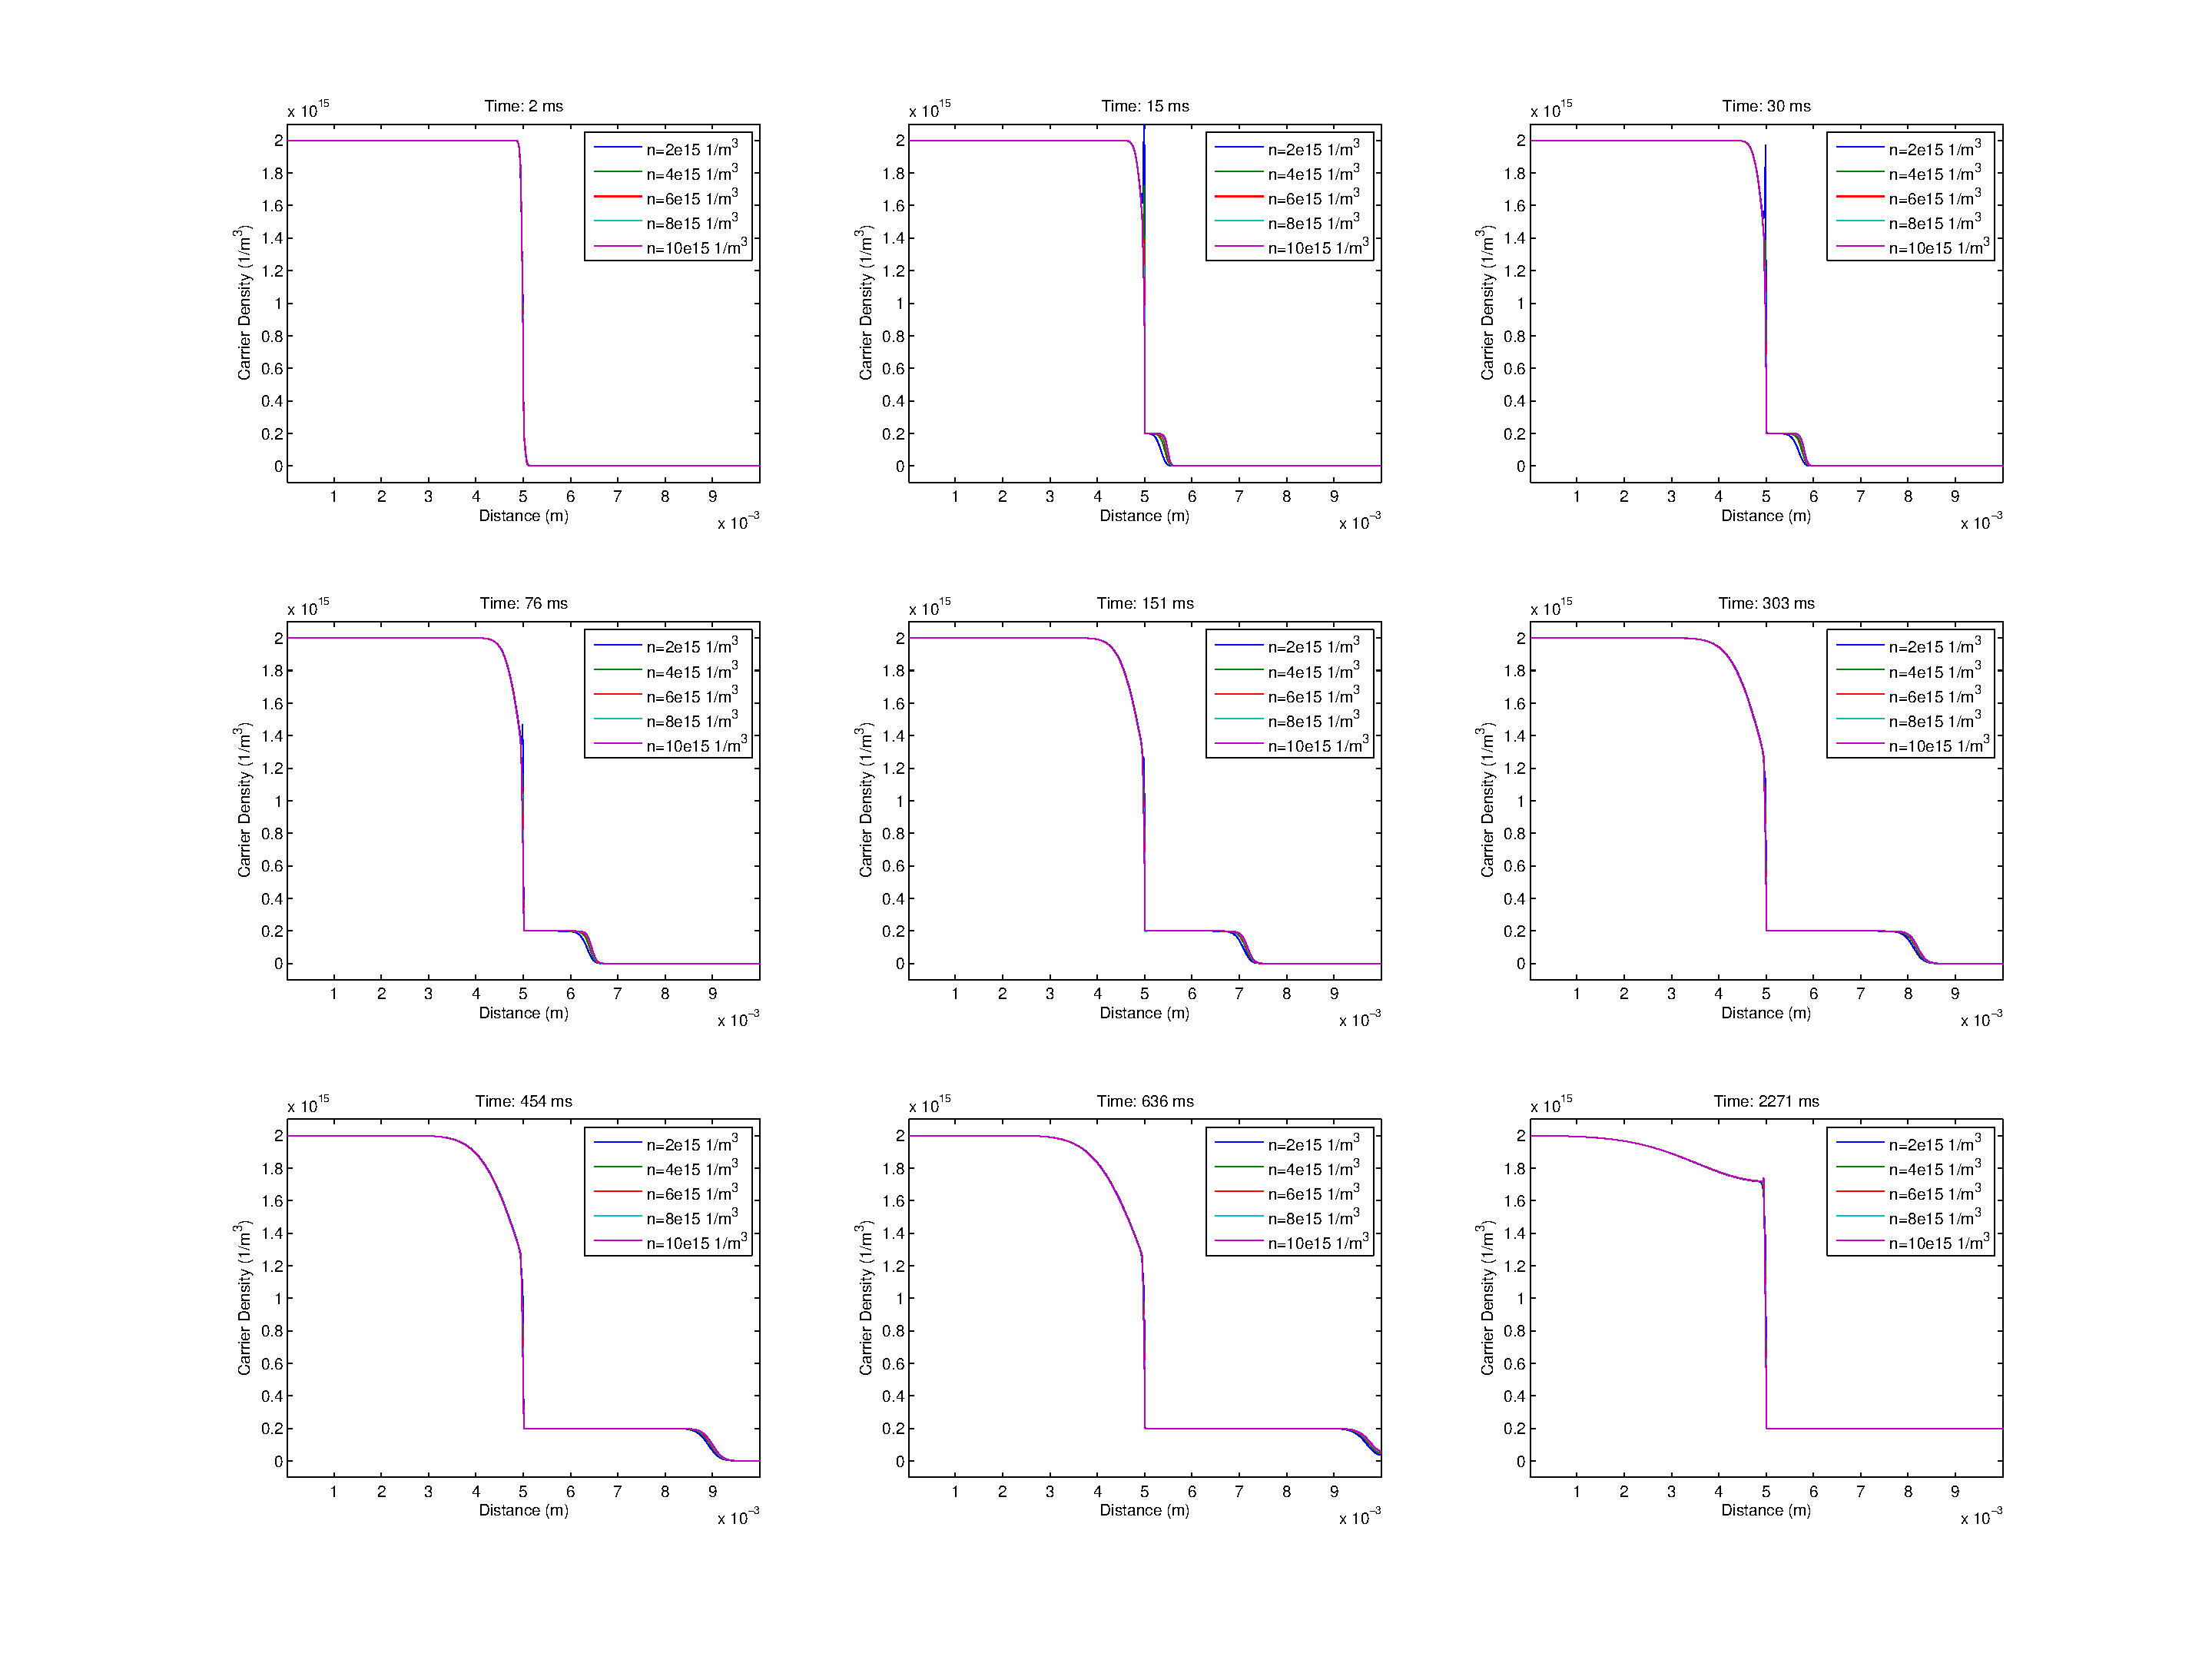
\includegraphics[scale=0.40]{Ex4Np_Time}
\caption{} 
\label{}
\end{figure}
\end{landscape}

\begin{landscape}
\begin{figure}[!htp]
\centering
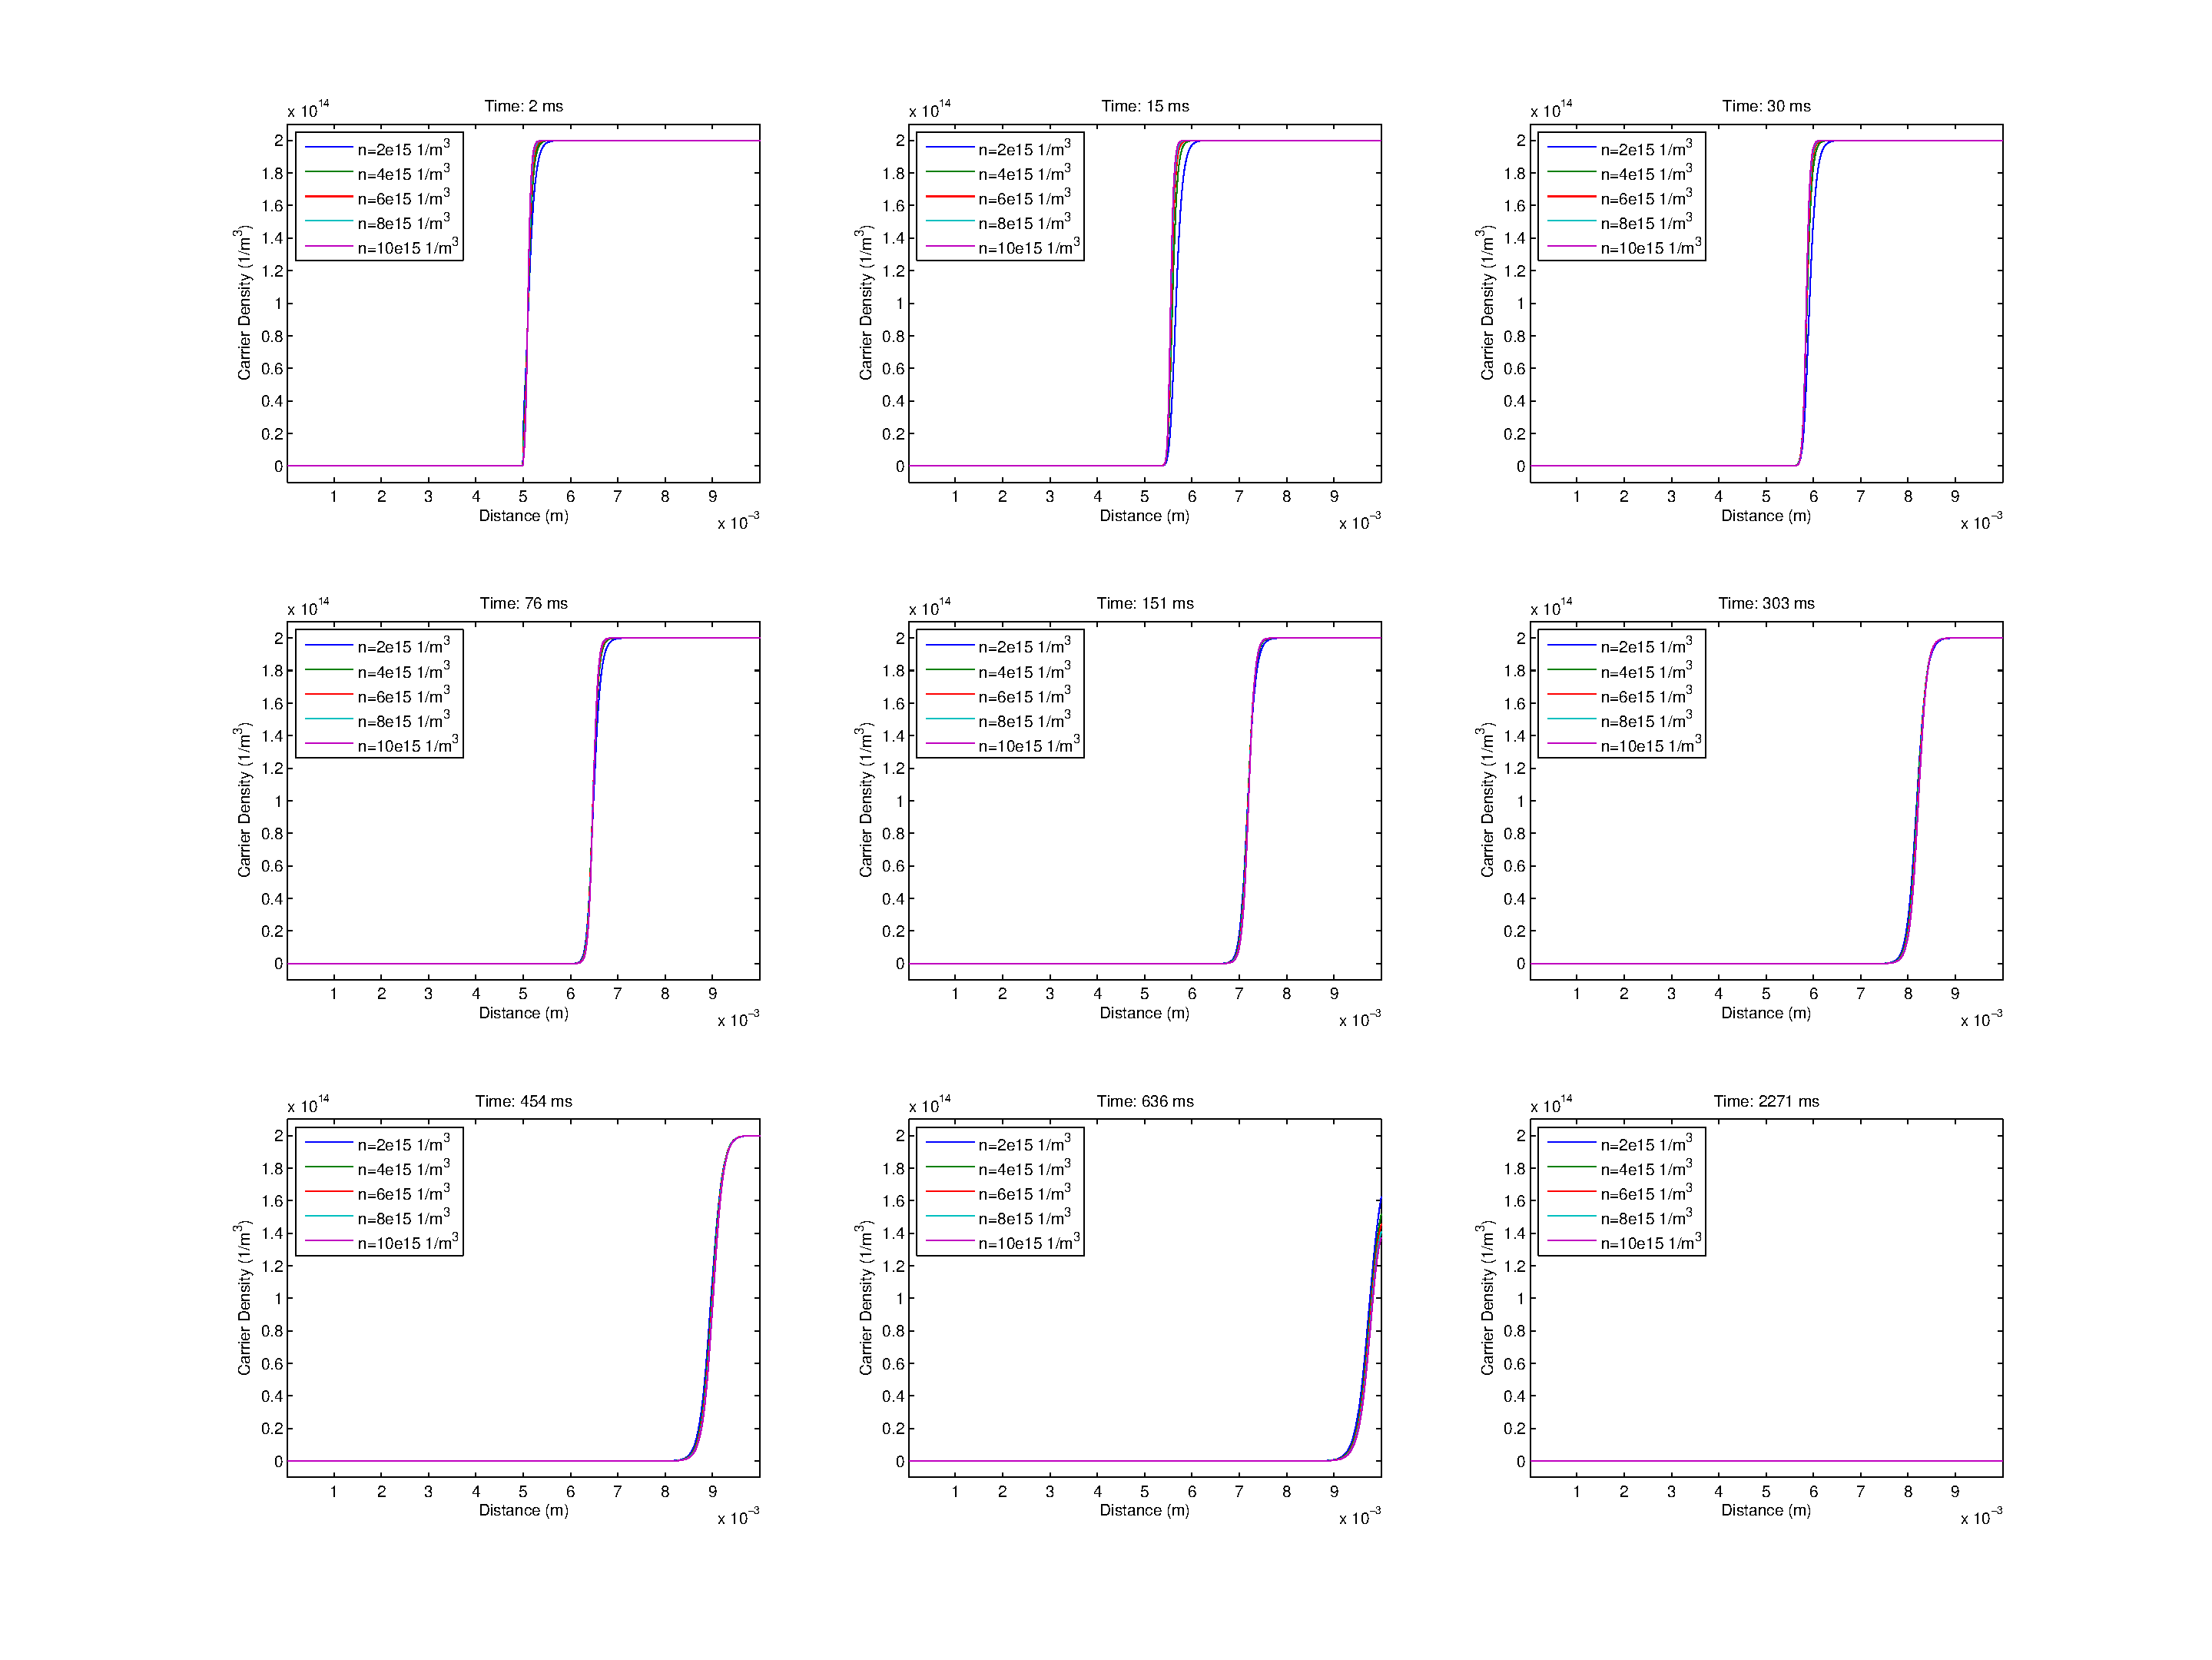
\includegraphics[scale=0.40]{Ex4p_Time}
\caption{} 
\label{}
\end{figure}
\end{landscape}

\begin{landscape}
\begin{figure}[!htp]
\centering
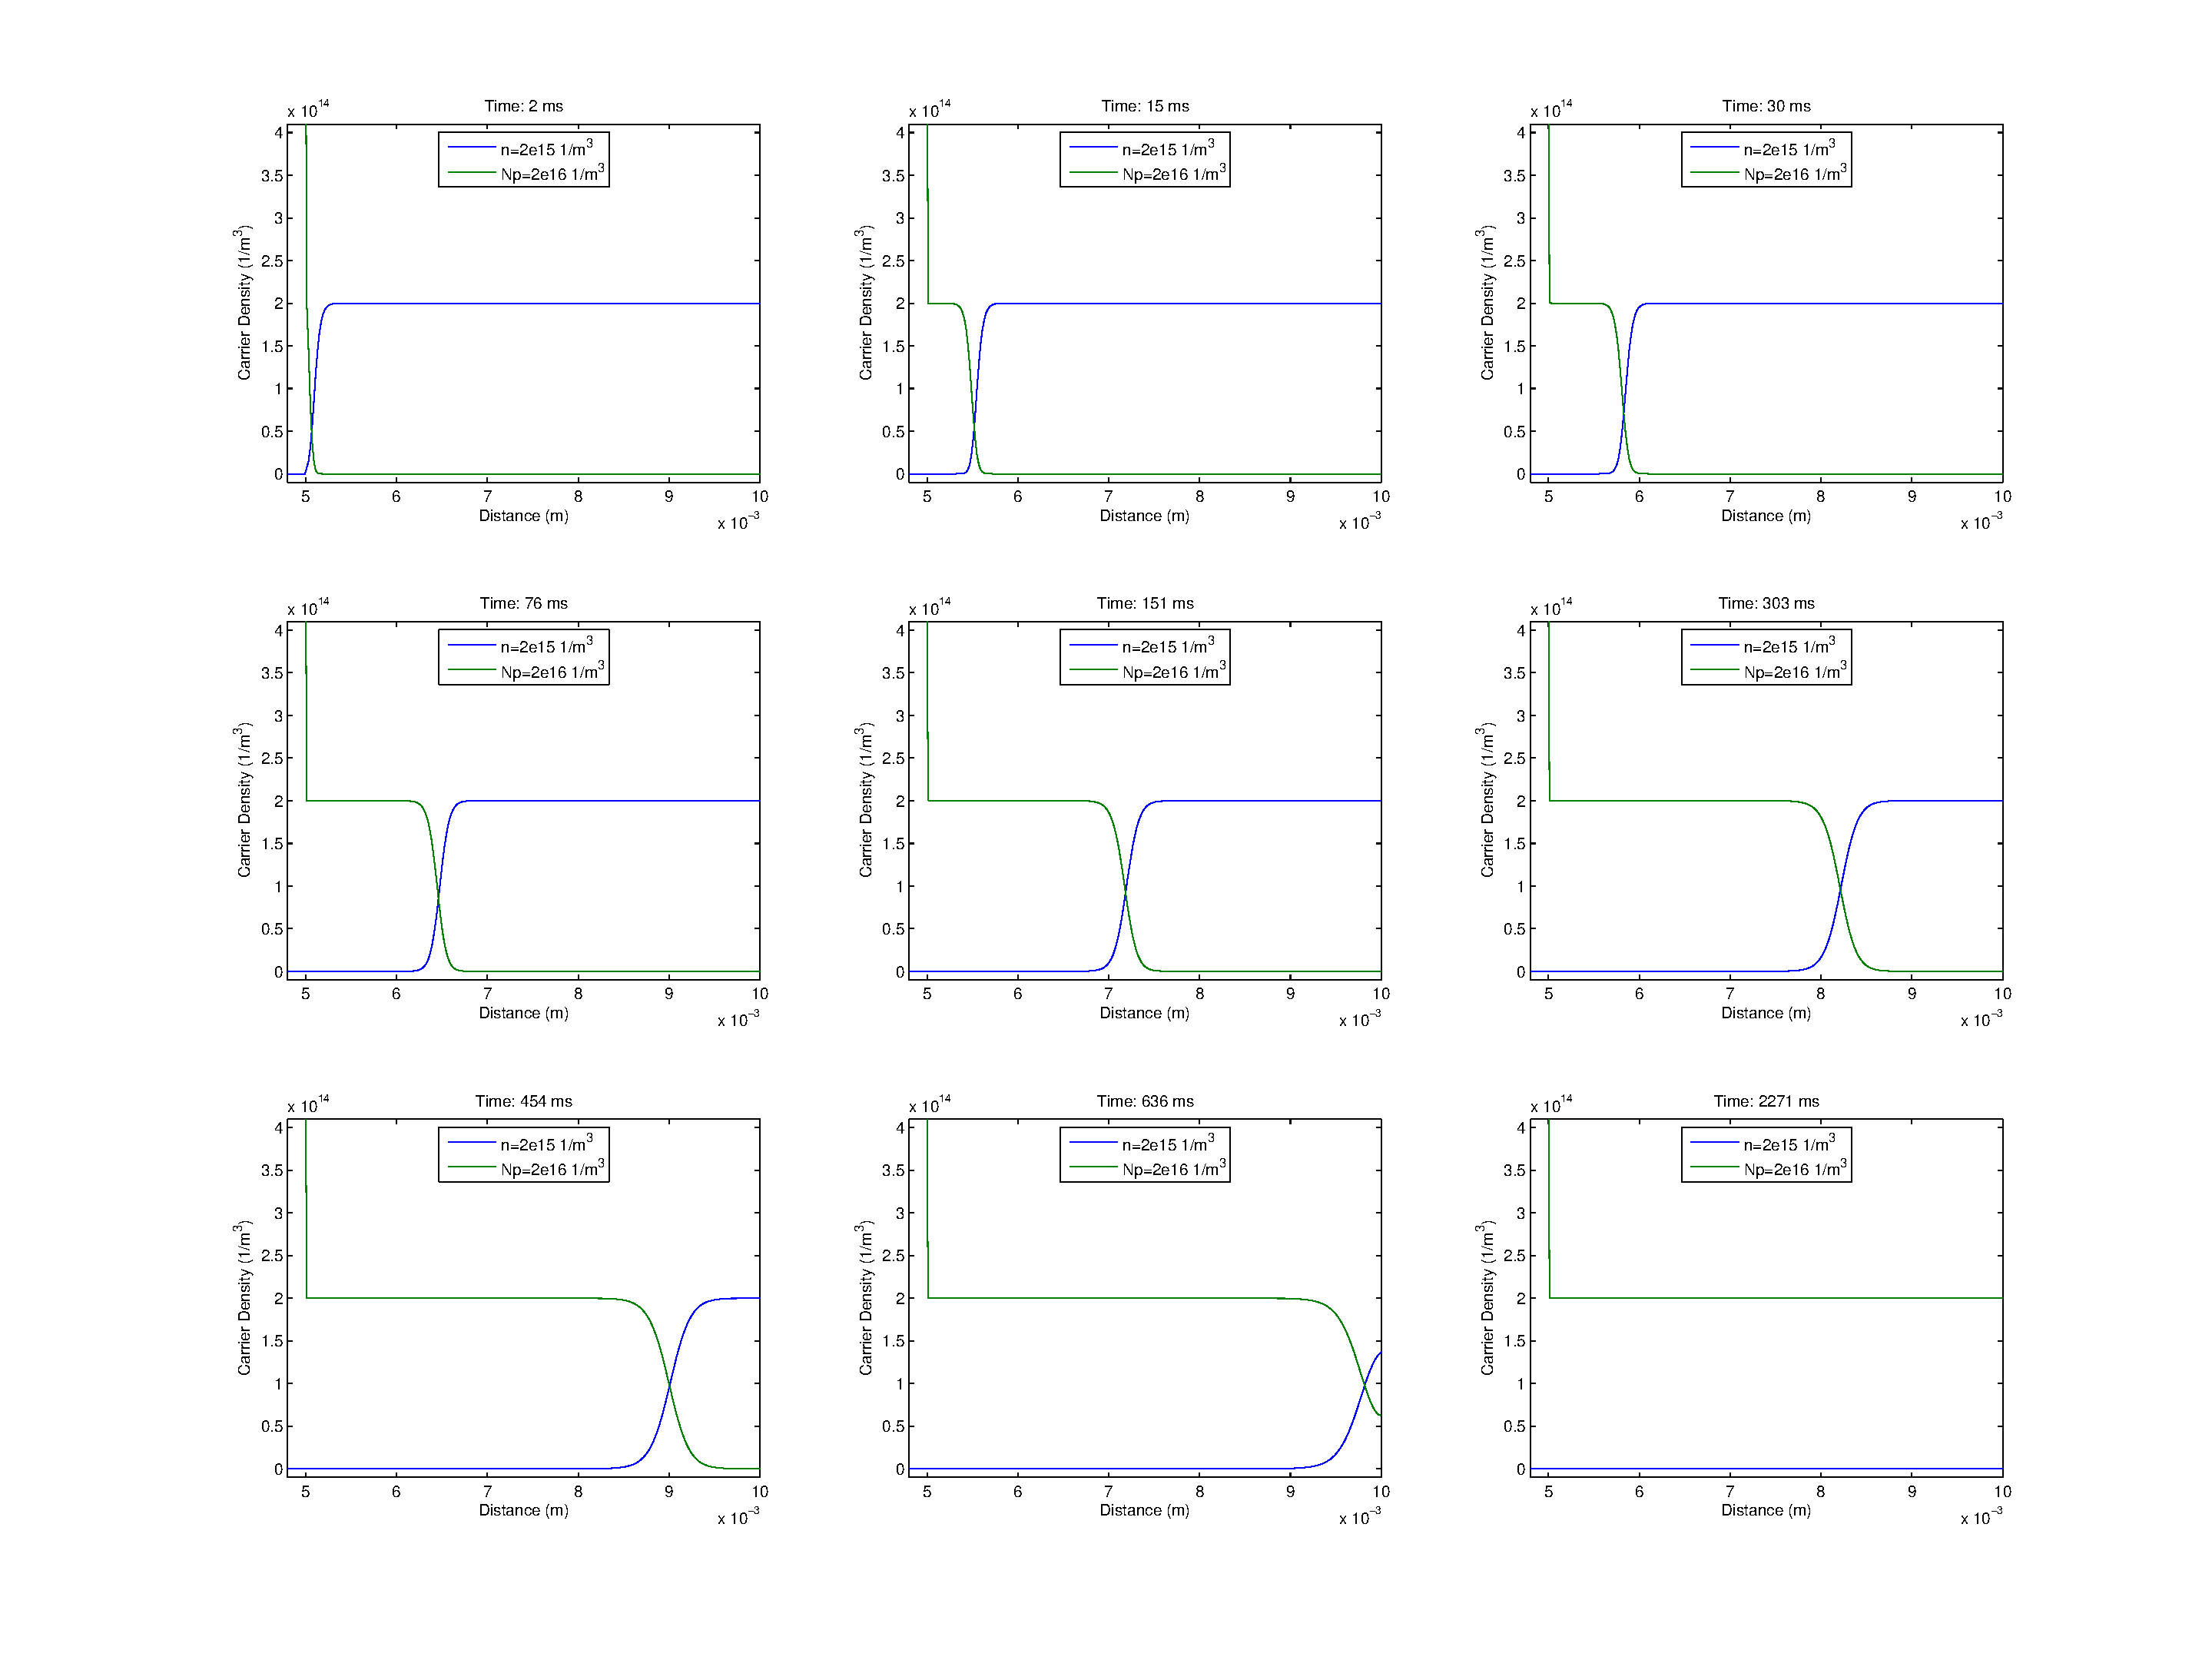
\includegraphics[scale=0.40]{Ex4pNp_Time}
\caption{} 
\label{}
\end{figure}
\end{landscape}

\begin{landscape}
\begin{figure}[!htp]
\centering
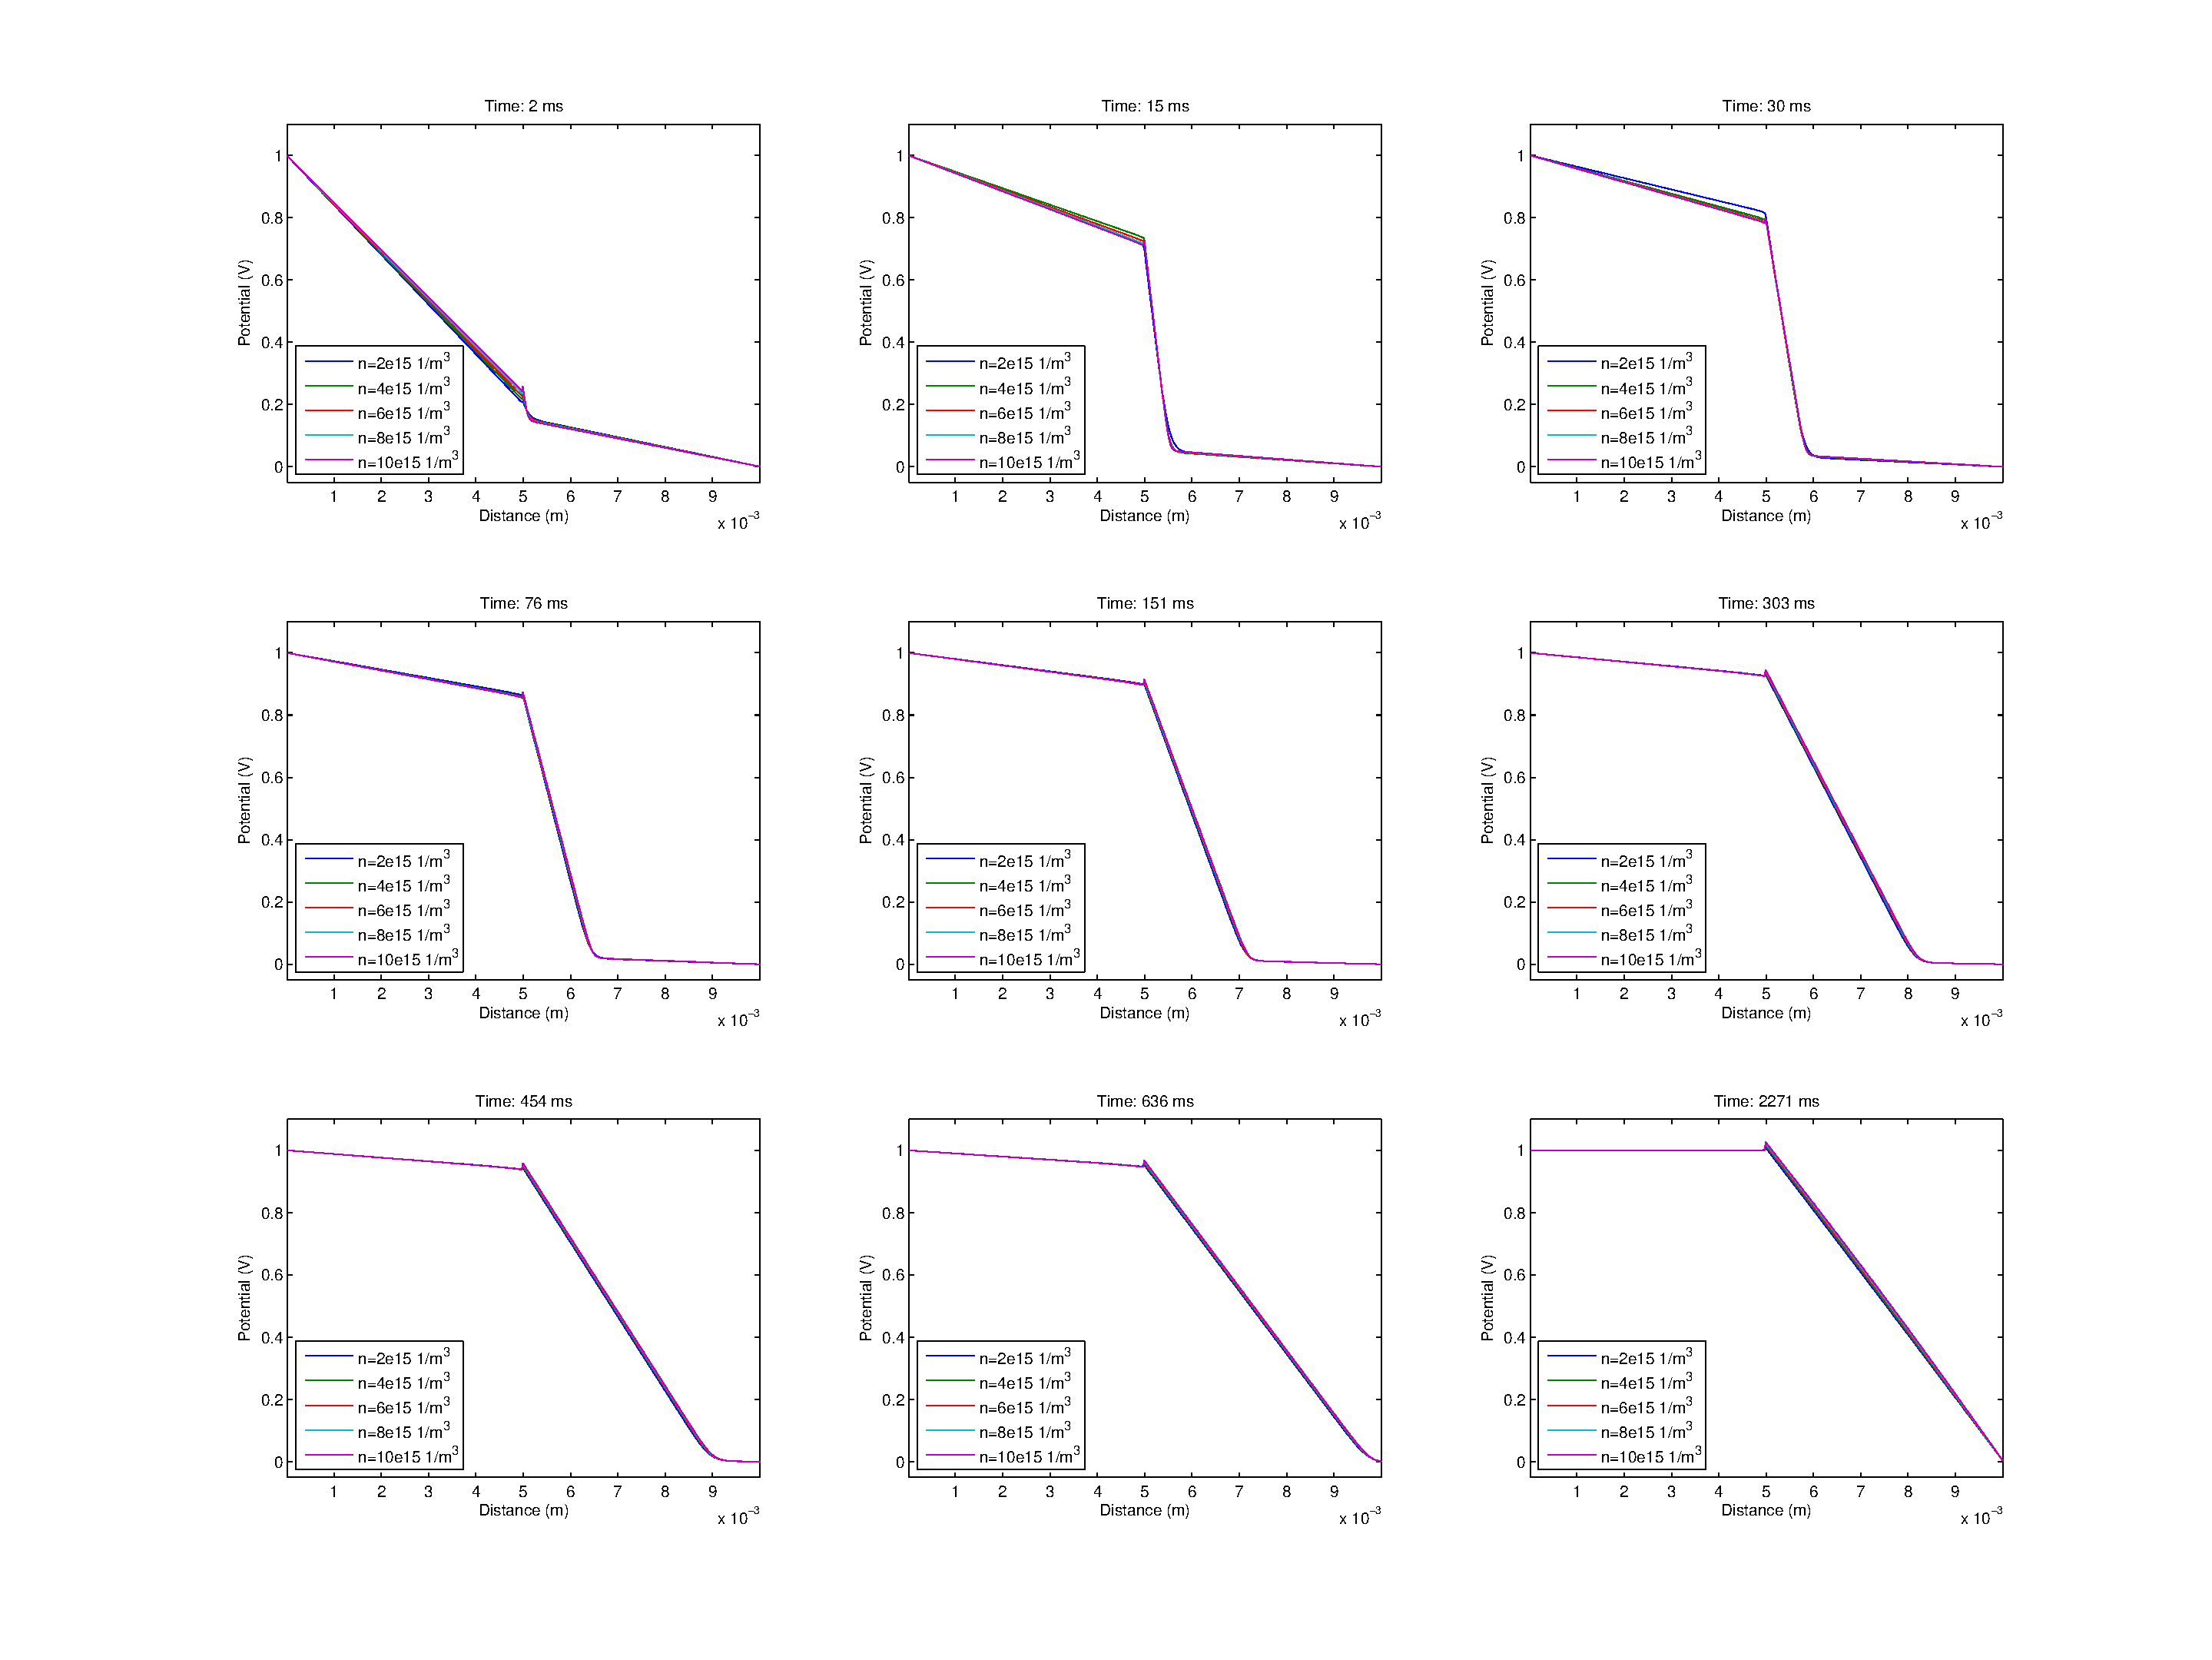
\includegraphics[scale=0.40]{Ex4V_Time}
\caption{} 
\label{}
\end{figure}
\end{landscape}




%1-D Vertical Medium and high concentration (hole freeze,# of holes over time)
%1-D Horizontal medium and high concentration (Add memristor pictures,hole freeze,# of holes over time)
